\documentclass{report}
\usepackage{inputenc}
\usepackage{comment}
\usepackage{fontspec}
\usepackage{authblk}
\usepackage{graphicx}
\usepackage{fancyhdr}
\usepackage{amssymb}
\usepackage{amsmath}
\usepackage{gensymb}
\usepackage{float}
\usepackage{enumerate}
\usepackage{tocloft}
\usepackage{abstract}
\usepackage[hidelinks]{hyperref}
\usepackage{appendix}
\usepackage[dvipsnames, svgnames, x11names]{xcolor}
\usepackage{dirtree}
\usepackage{cite}
\usepackage{geometry}
\usepackage{makecell}
\usepackage{multirow}
\usepackage{graphicx}
\usepackage{float}
\usepackage{subfig}
% \usepackage[hmargin={3.18cm, 3.18cm}, width=14.64cm, vmargin={2.54cm, 2.54cm}, height=24.62cm]{geometry}
\usepackage[ruled]{algorithm2e}

\pagestyle{fancy}

\renewcommand\thesection{\arabic{section}}

\newcommand*{\rmd}{\mathop{}\!\mathrm{d}}
\newcommand*{\sgn}{\mathrm{sgn}}
\renewcommand{\cftsecleader}{\cftdotfill{\cftdotsep}}

\title{\Huge A title is all you need}

\author{
    \parbox{0.2\textwidth}{
        \centering Name 1 \\
        \centering Student No 1
    }
    \parbox{0.2\textwidth}{
        \centering Name 2 \\
        \centering Student No 2
    }
    \parbox{0.2\textwidth}{
        \centering Name 3 \\
        \centering Student No 3
    }
    \parbox{0.2\textwidth}{
        \centering Name 4 \\
        \centering Student No 4
    }
}

\date{\today}

\setcounter{tocdepth}{2}
\setcounter{secnumdepth}{3}

\begin{document}

\maketitle

\tableofcontents
\thispagestyle{empty}
\setcounter{page}{0}

\newpage

\section{Introduction}

\subsection{Sex difference}

\subsection{Functional Connectivity}

\subsection{Neural Network}

\section{Materials and methods}

\subsection{Human Connectome Project (HCP)}

\subsection{Data Preprocessing}

\begin{figure}[H]
    \centering
    \subfloat[]{\includegraphics[width=0.3\textwidth]{../Analysis/Dynamic/node=15_id=100206/0_1.jpg}}
    \subfloat[]{\includegraphics[width=0.3\textwidth]{../Analysis/Dynamic/node=25_id=100206/0_1.jpg}}
    \subfloat[]{\includegraphics[width=0.3\textwidth]{../Analysis/Dynamic/node=50_id=100206/0_1.jpg}} \\
    \subfloat[]{\includegraphics[width=0.3\textwidth]{../Analysis/Dynamic/node=15_id=100307/0_2.jpg}}
    \subfloat[]{\includegraphics[width=0.3\textwidth]{../Analysis/Dynamic/node=25_id=100307/0_2.jpg}}
    \subfloat[]{\includegraphics[width=0.3\textwidth]{../Analysis/Dynamic/node=50_id=100307/0_2.jpg}} \\
    \subfloat[]{\includegraphics[width=0.3\textwidth]{../Analysis/Dynamic/node=15_id=100307/0_3.jpg}}
    \subfloat[]{\includegraphics[width=0.3\textwidth]{../Analysis/Dynamic/node=25_id=100307/0_3.jpg}}
    \subfloat[]{\includegraphics[width=0.3\textwidth]{../Analysis/Dynamic/node=50_id=100307/0_3.jpg}} \\
    \caption{Dynamic connectivity with $N_{node} = 15, 25, 50$.}
    \label{Dynamic-example-1}
\end{figure}

\begin{table}[!htbp]
    \centering
    \begin{tabular}{|c|c|c|c|}
        \hline
                        & min                    & mean                  & max                   \\
        \hline
        $N_{node} = 15$ & 1.366036853342154e-05  & 2.533653786919024e-05 & 6.491661970661407e-05 \\
        \hline
        $N_{node} = 25$ & 5.204765189263073e-06  & 9.253529597727324e-06 & 1.935569050475904e-05 \\
        \hline
        $N_{node} = 50$ & 1.0647490177903414e-07 & 9.65062448973428e-07  & 2.054828236469856e-06 \\
        \hline
    \end{tabular}
    \label{table1}
    \caption{Variance}
\end{table}

\subsection{Linear discriminant analysis (LDA)}

\begin{figure}[H]
    \centering
    \subfloat[]{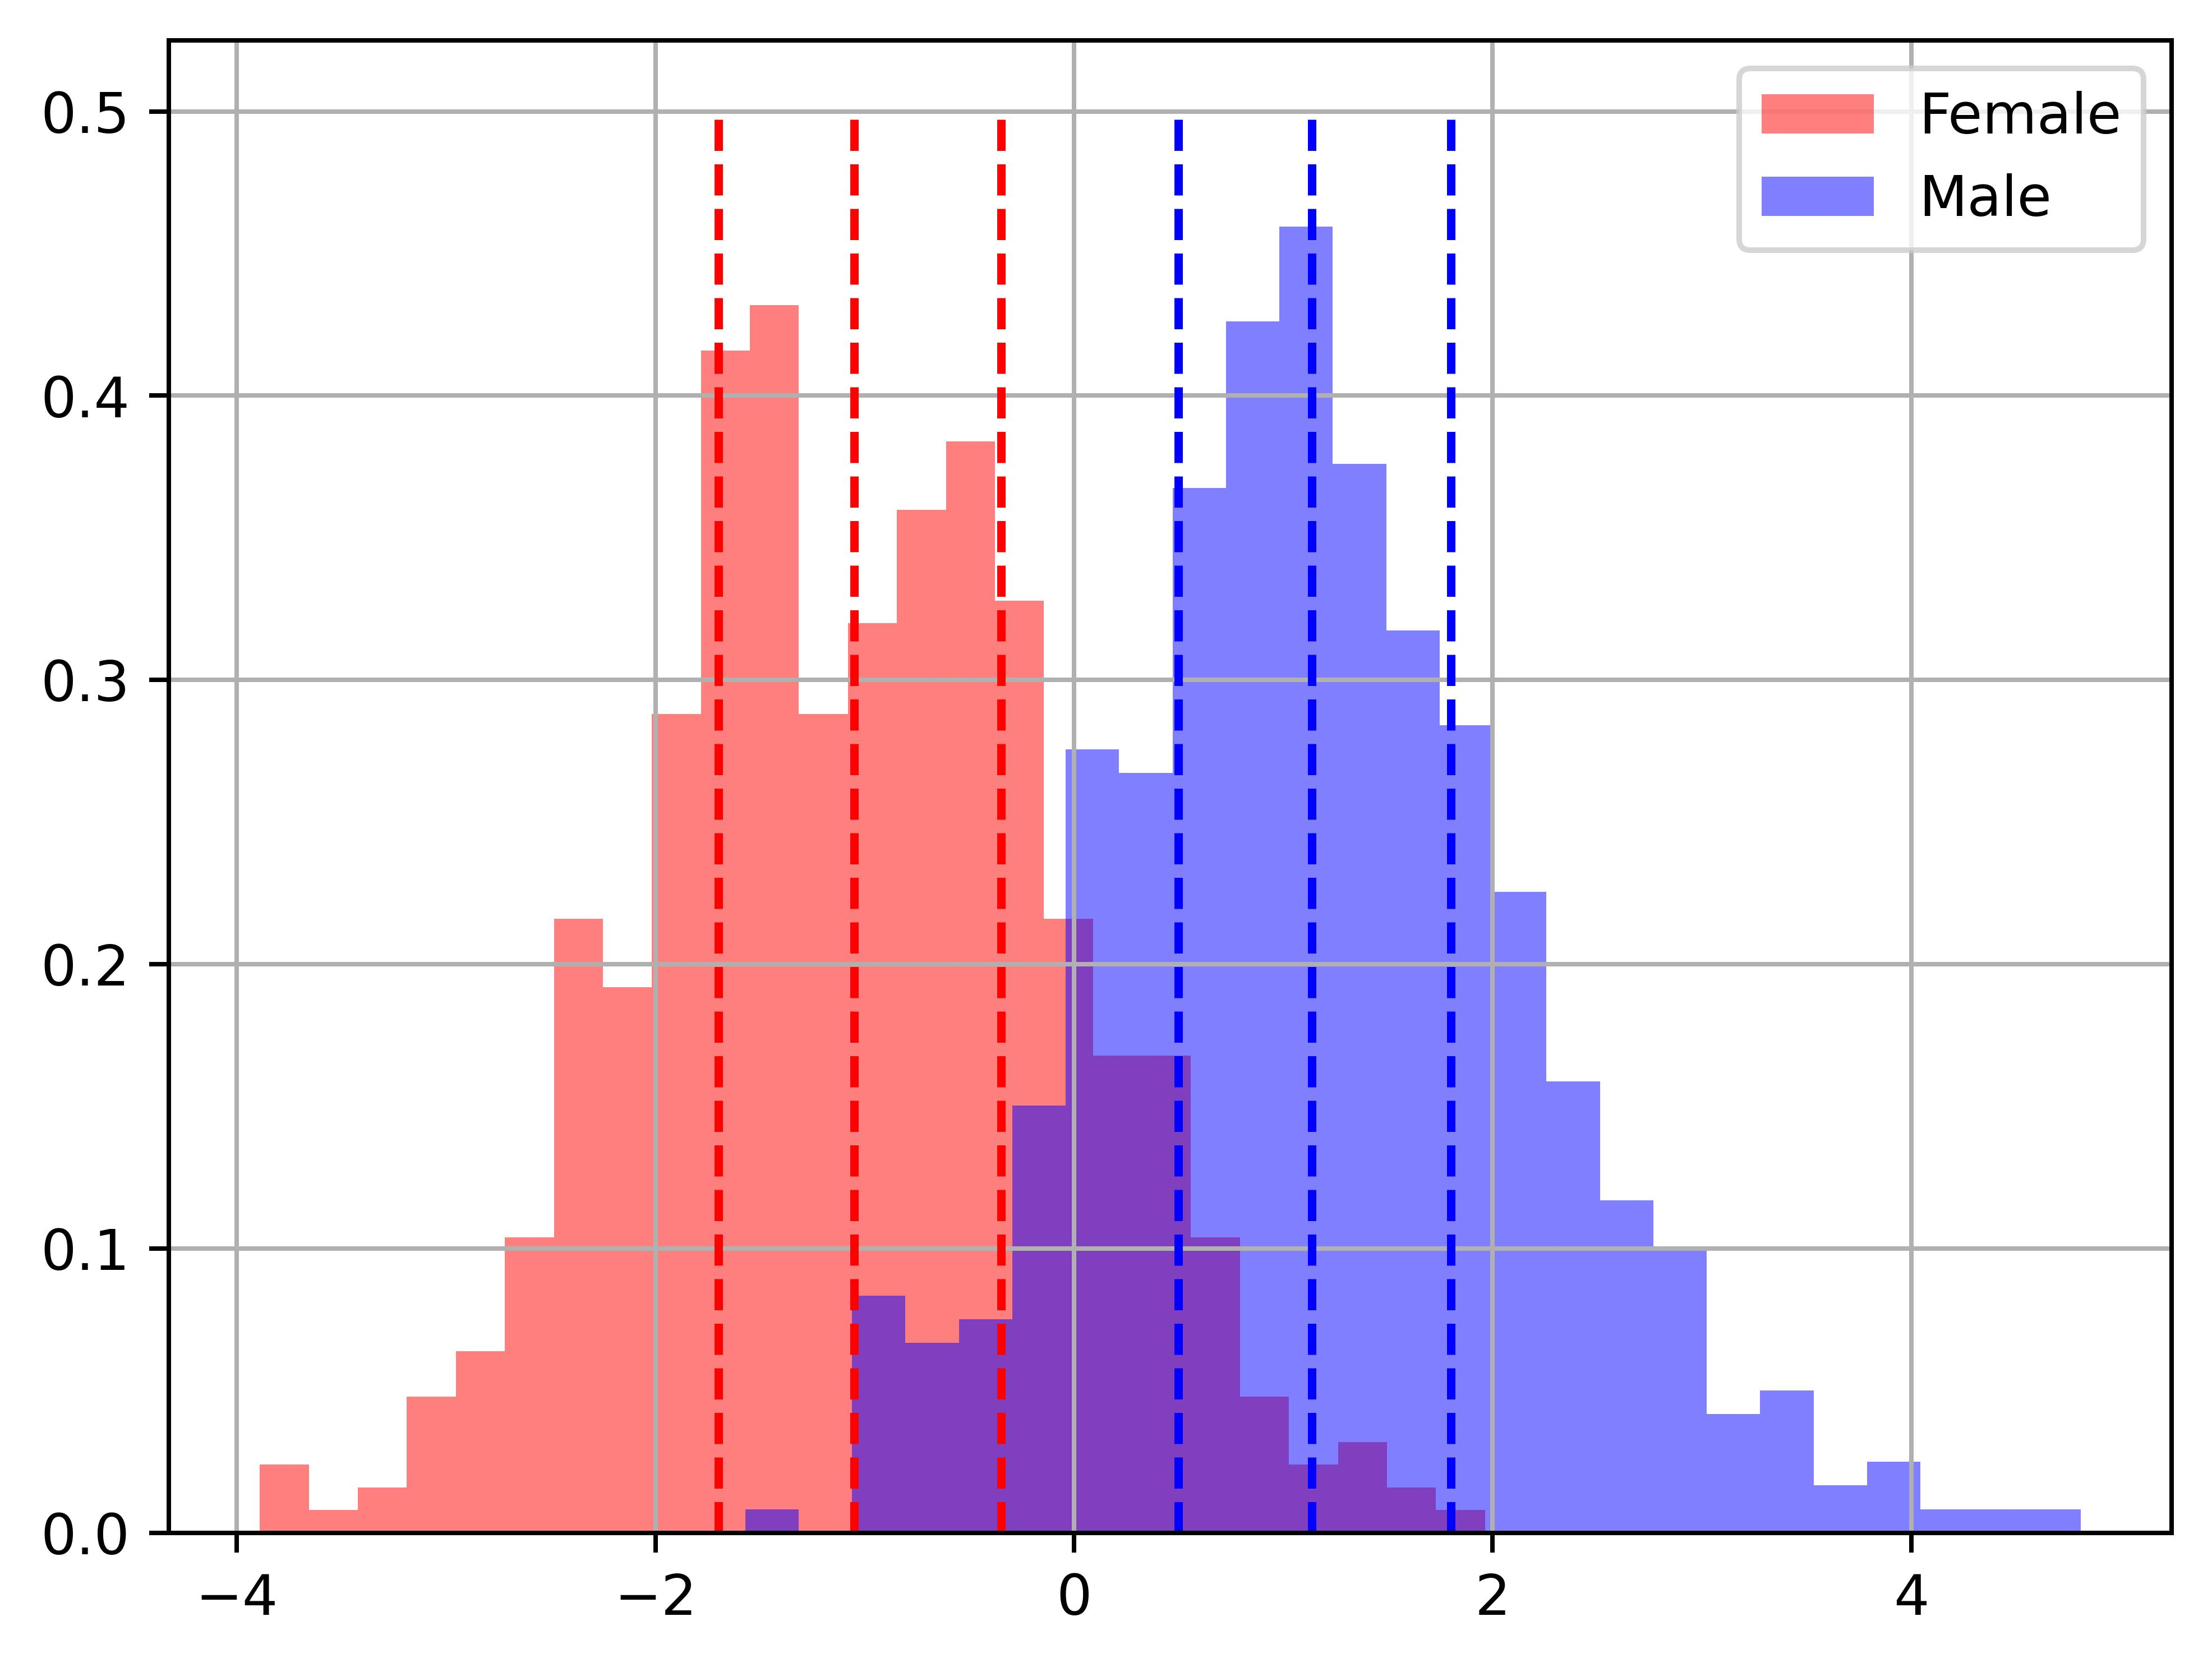
\includegraphics[width=0.4\textwidth]{../Analysis/LDA/node=15_size=4800_step=4800_rho=0.1/hist_0.jpg}}
    \subfloat[]{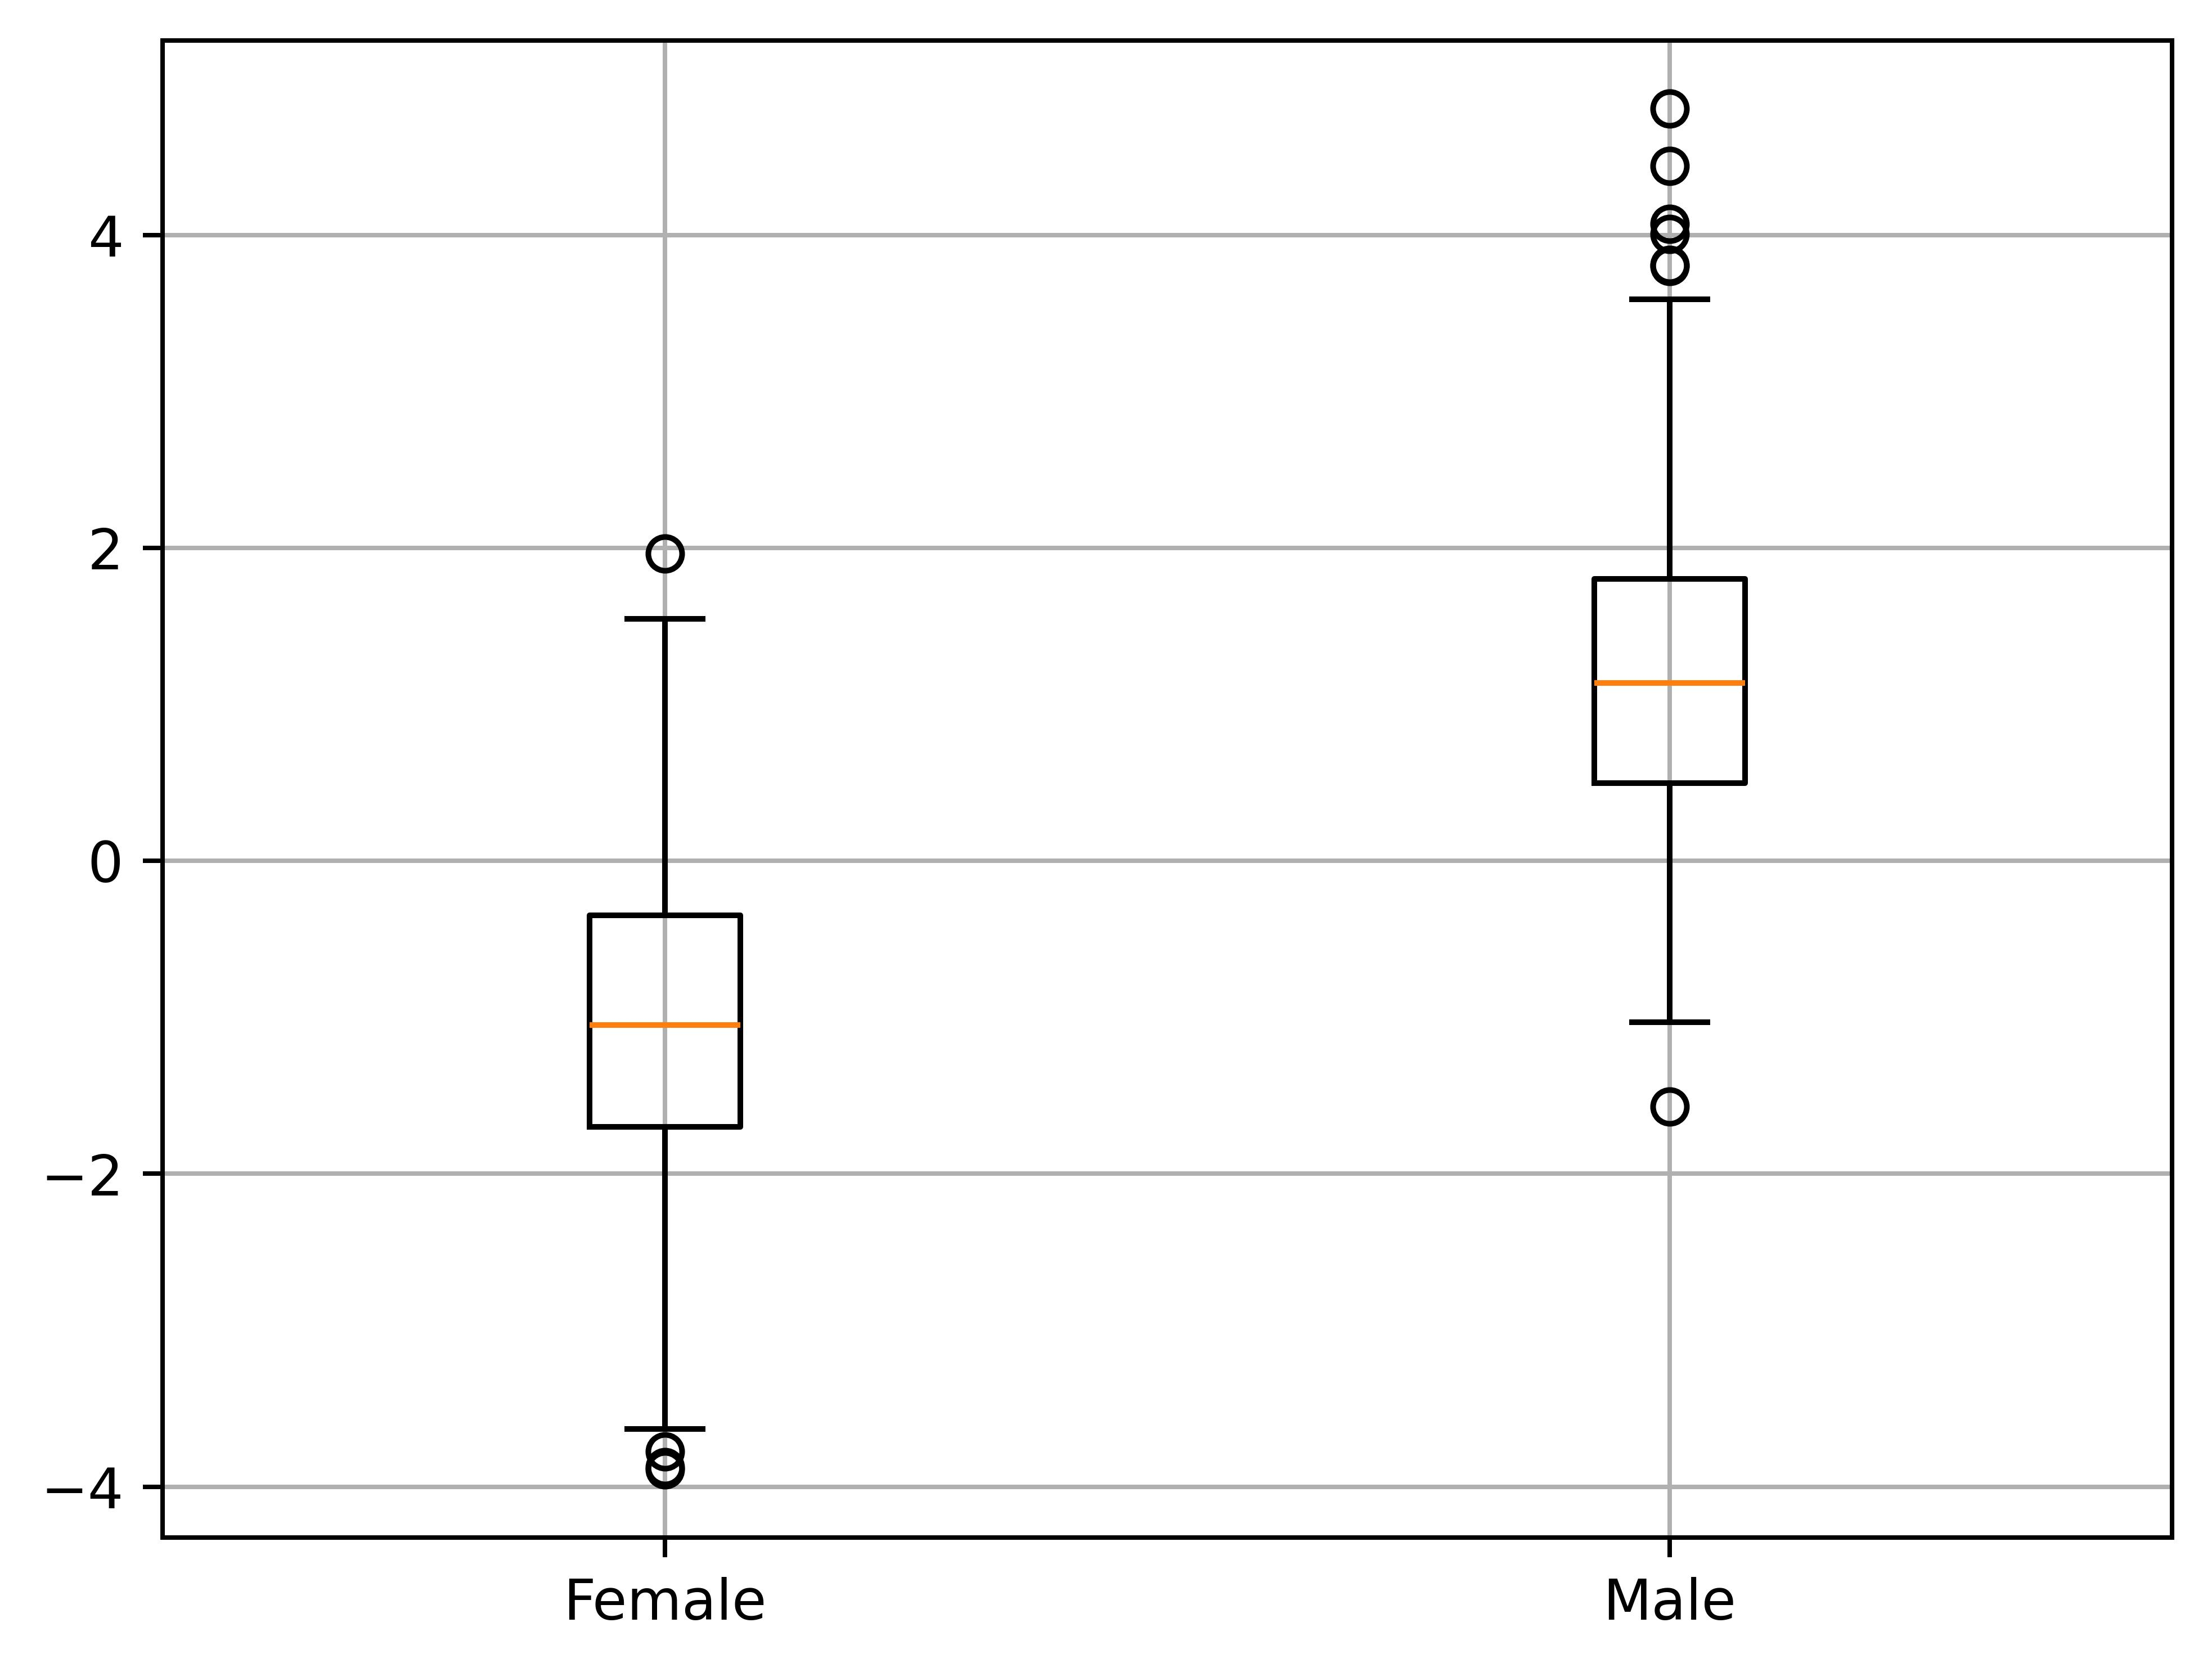
\includegraphics[width=0.4\textwidth]{../Analysis/LDA/node=15_size=4800_step=4800_rho=0.1/box_0.jpg}} \\
    \caption{LDA for static connectivity with $N_{node} = 15$.}
    \label{LDA-example-1}
\end{figure}

\begin{figure}[H]
    \centering
    \subfloat[]{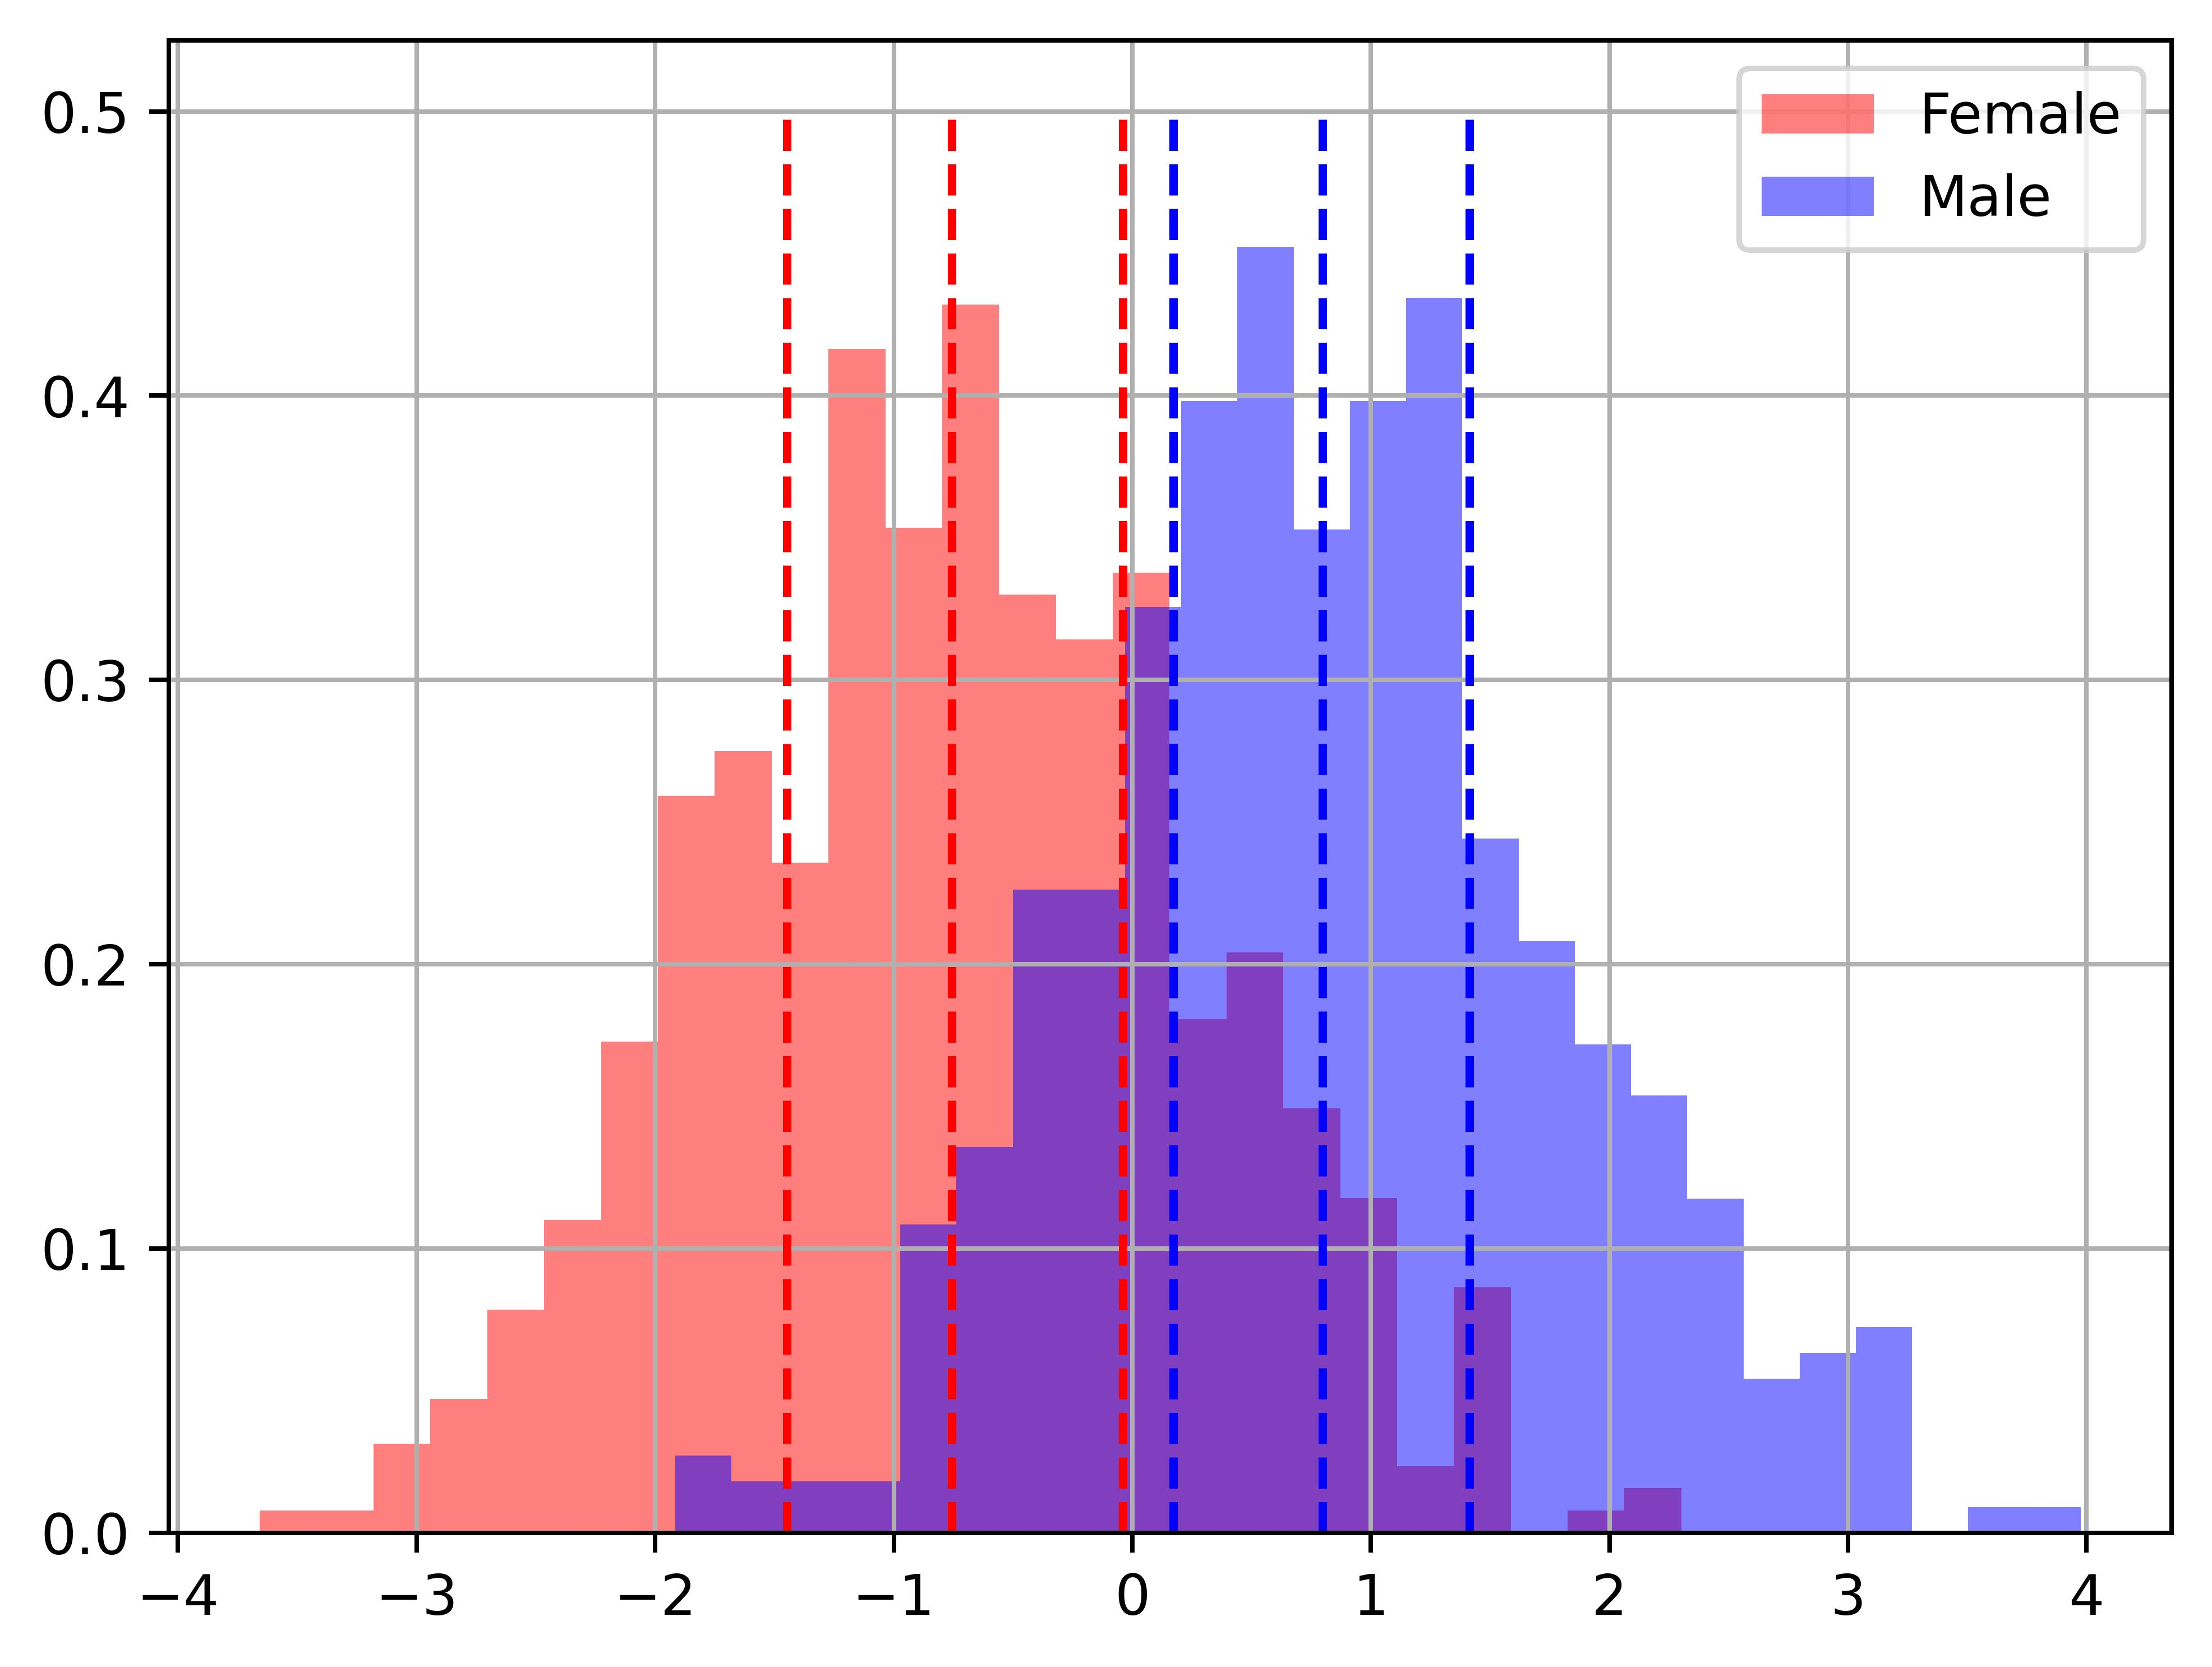
\includegraphics[width=0.4\textwidth]{../Analysis/LDA/node=15_size=480_step=180_rho=0.1/hist_0.jpg}}
    \subfloat[]{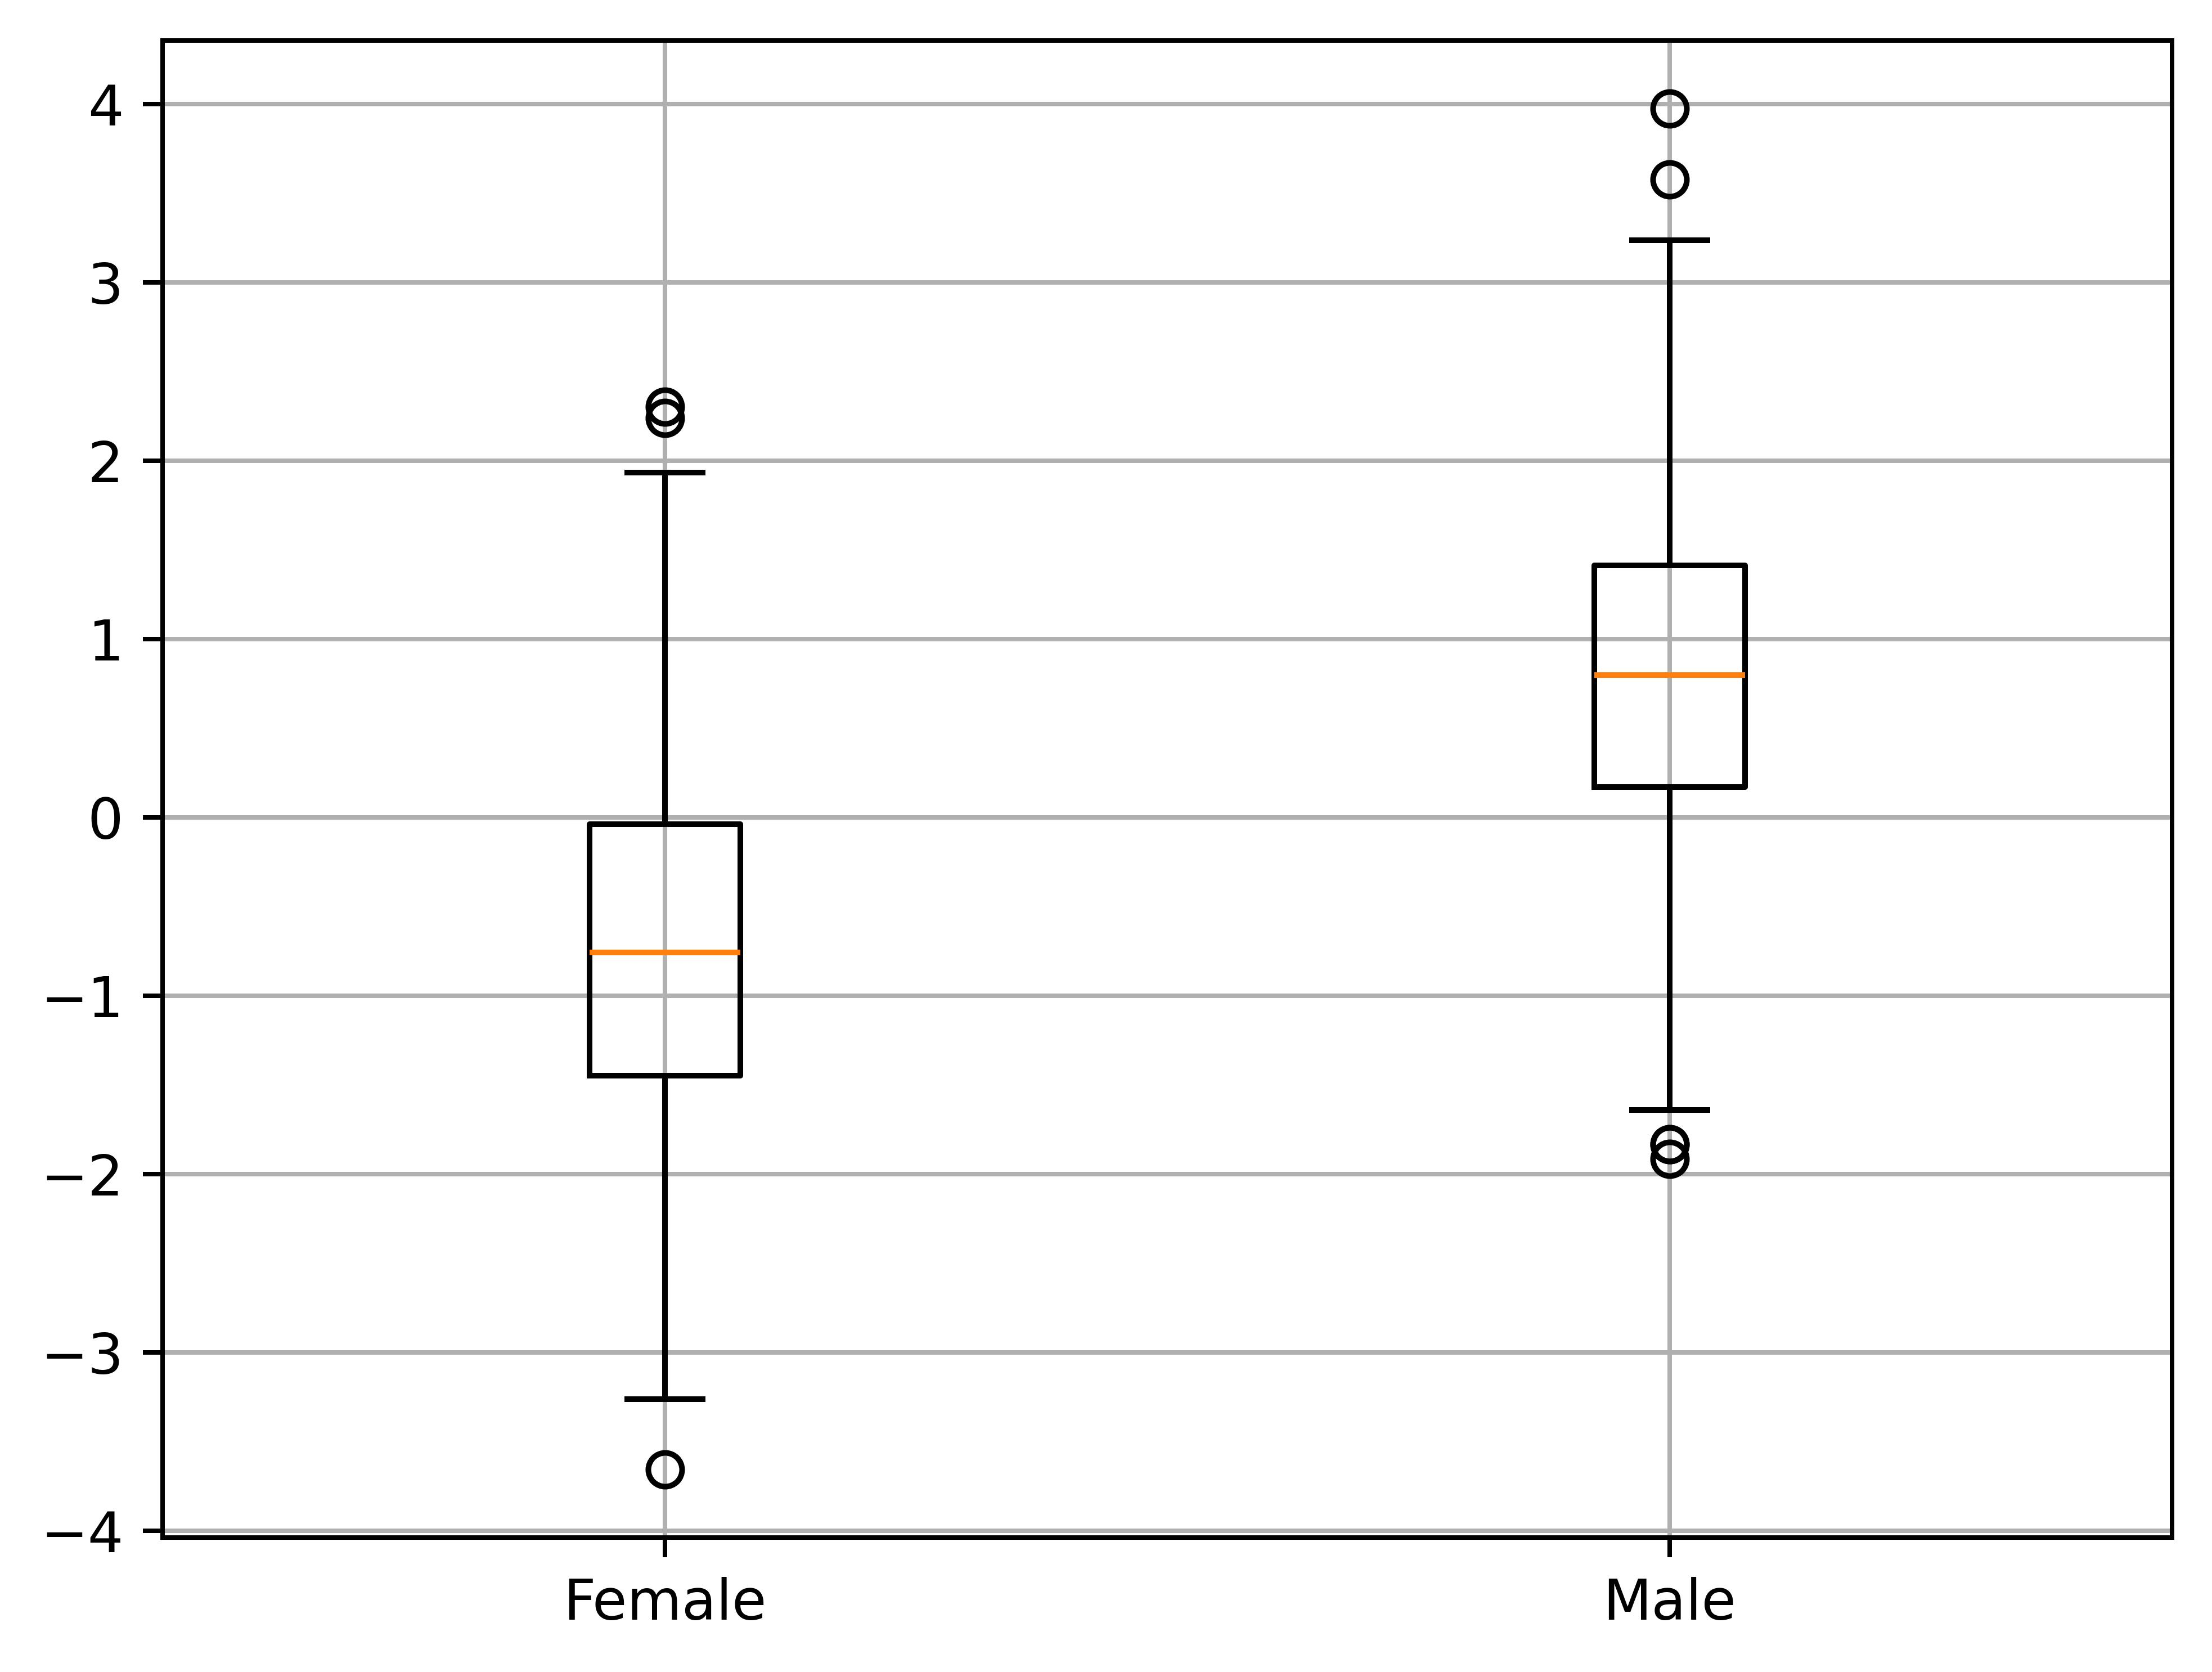
\includegraphics[width=0.4\textwidth]{../Analysis/LDA/node=15_size=480_step=180_rho=0.1/box_0.jpg}} \\
    \subfloat[]{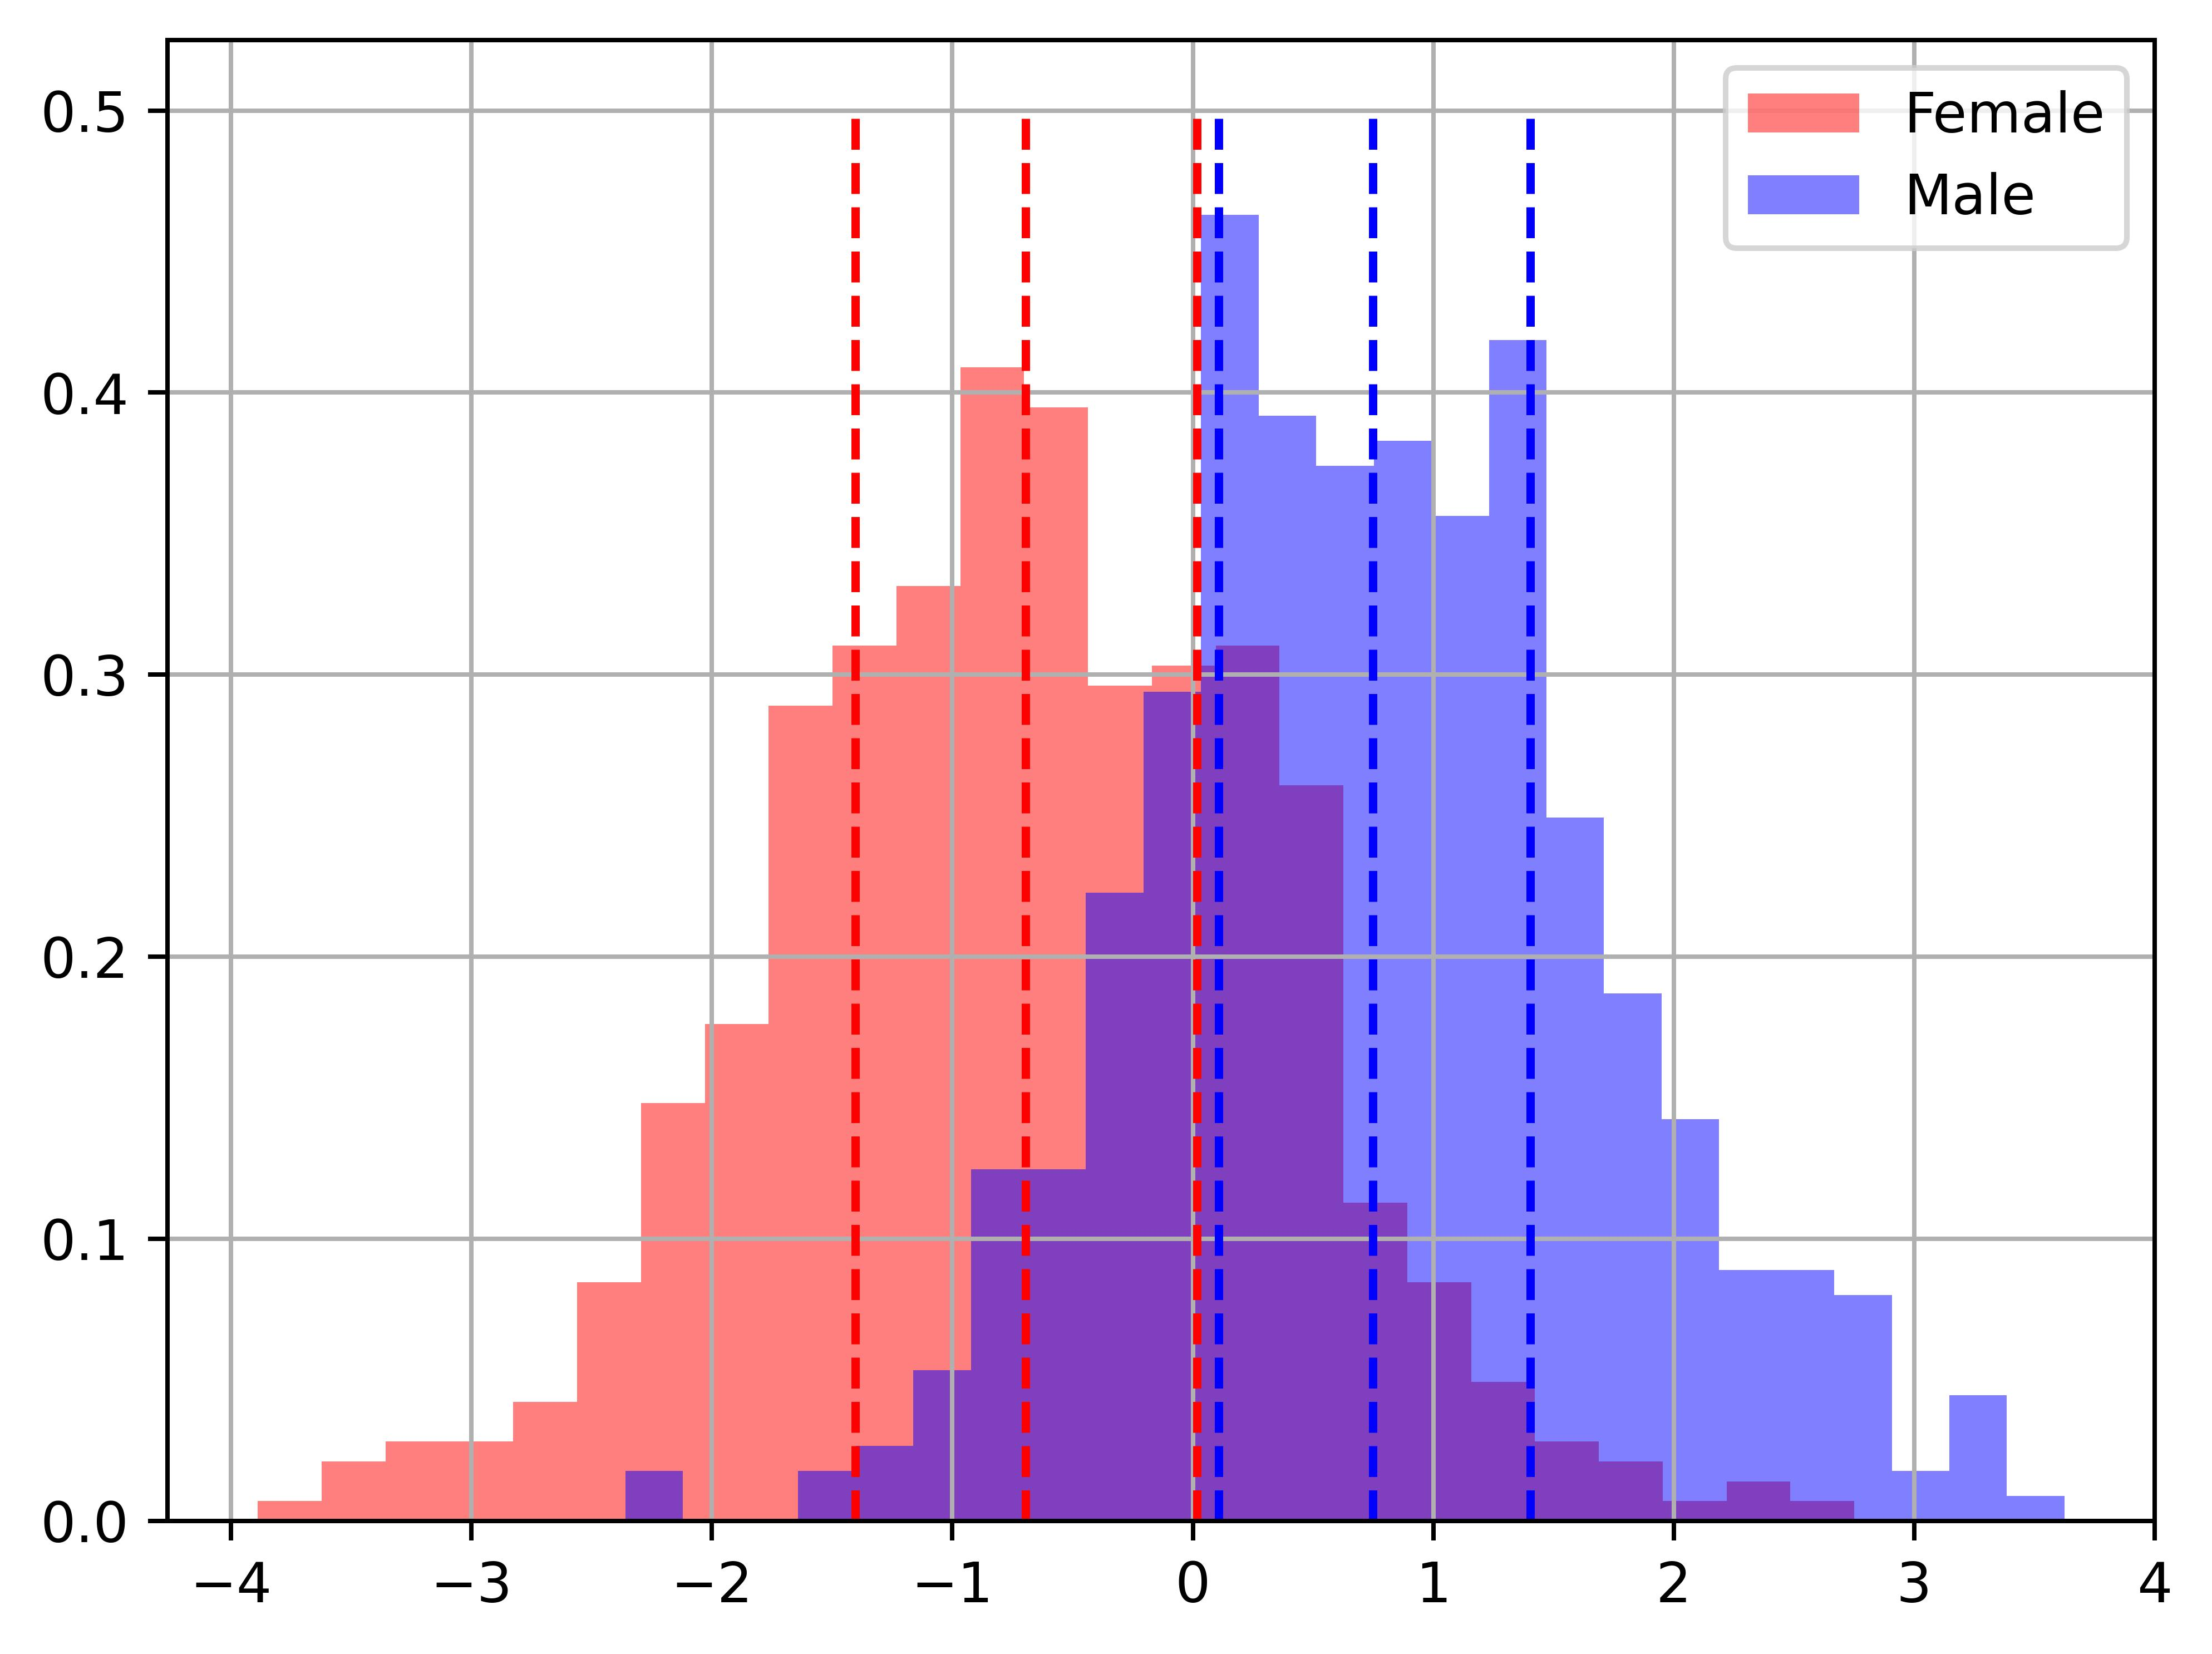
\includegraphics[width=0.4\textwidth]{../Analysis/LDA/node=15_size=480_step=180_rho=0.1/hist_1.jpg}}
    \subfloat[]{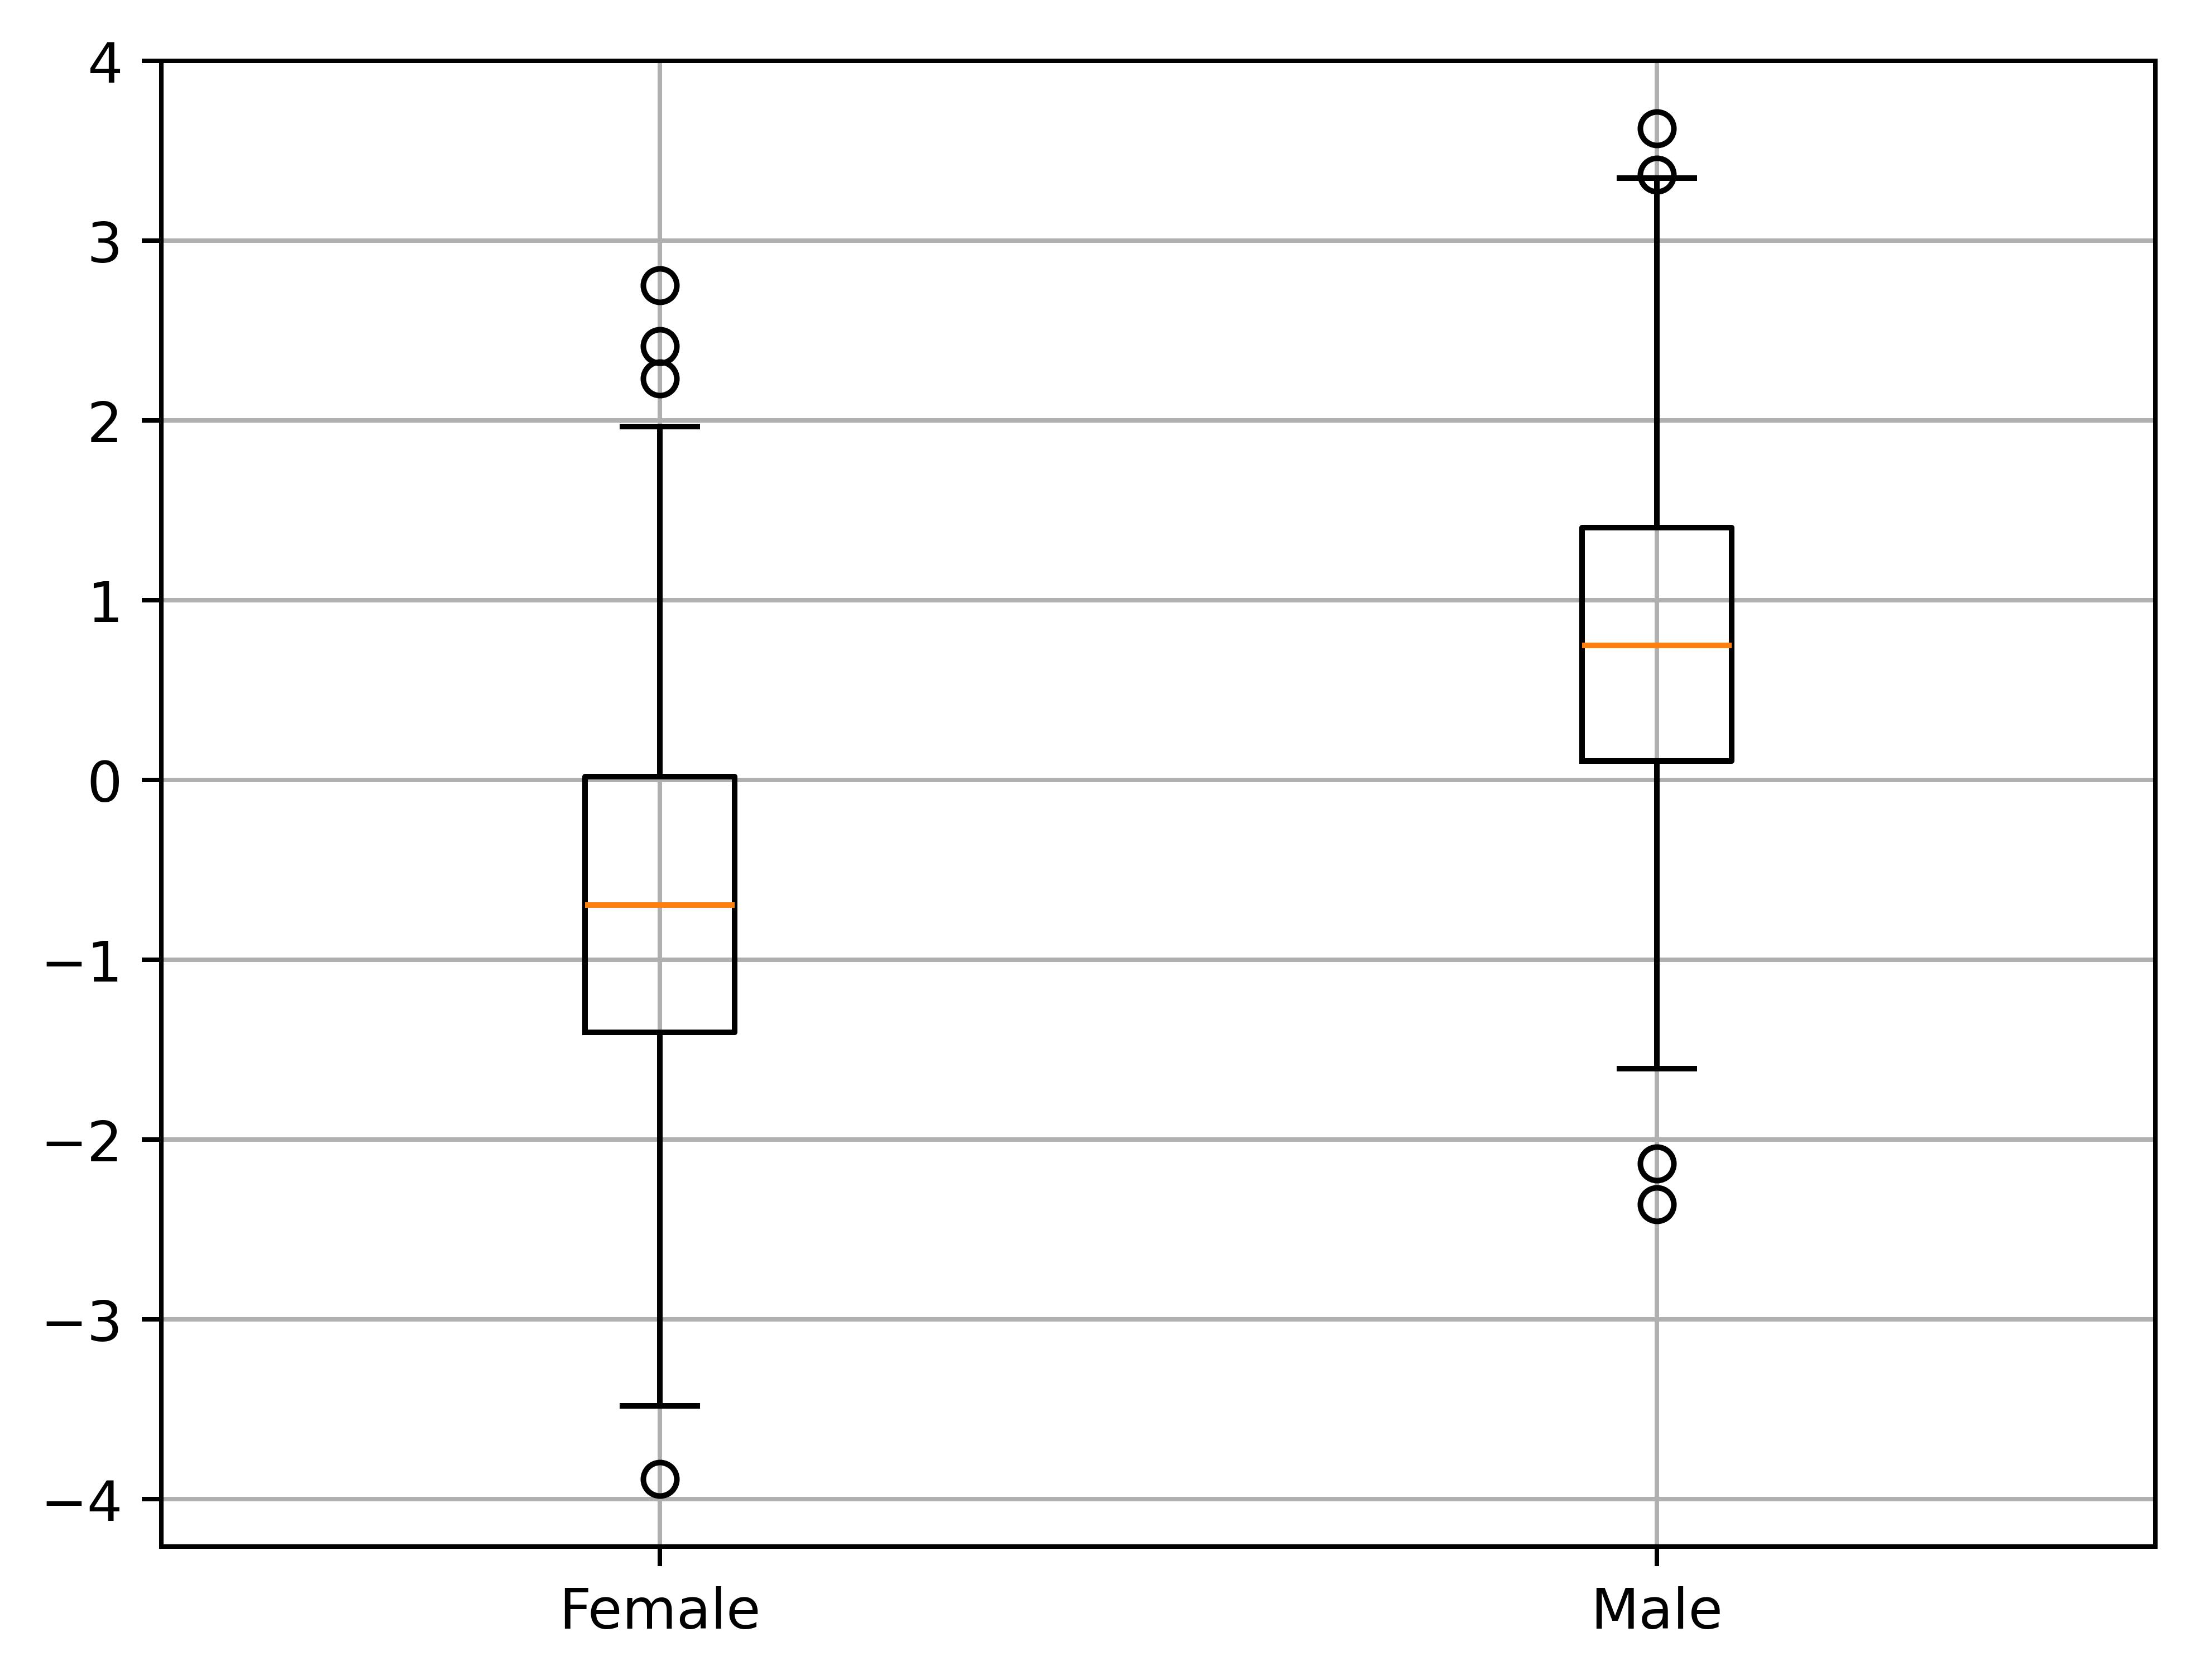
\includegraphics[width=0.4\textwidth]{../Analysis/LDA/node=15_size=480_step=180_rho=0.1/box_1.jpg}} \\
    \subfloat[]{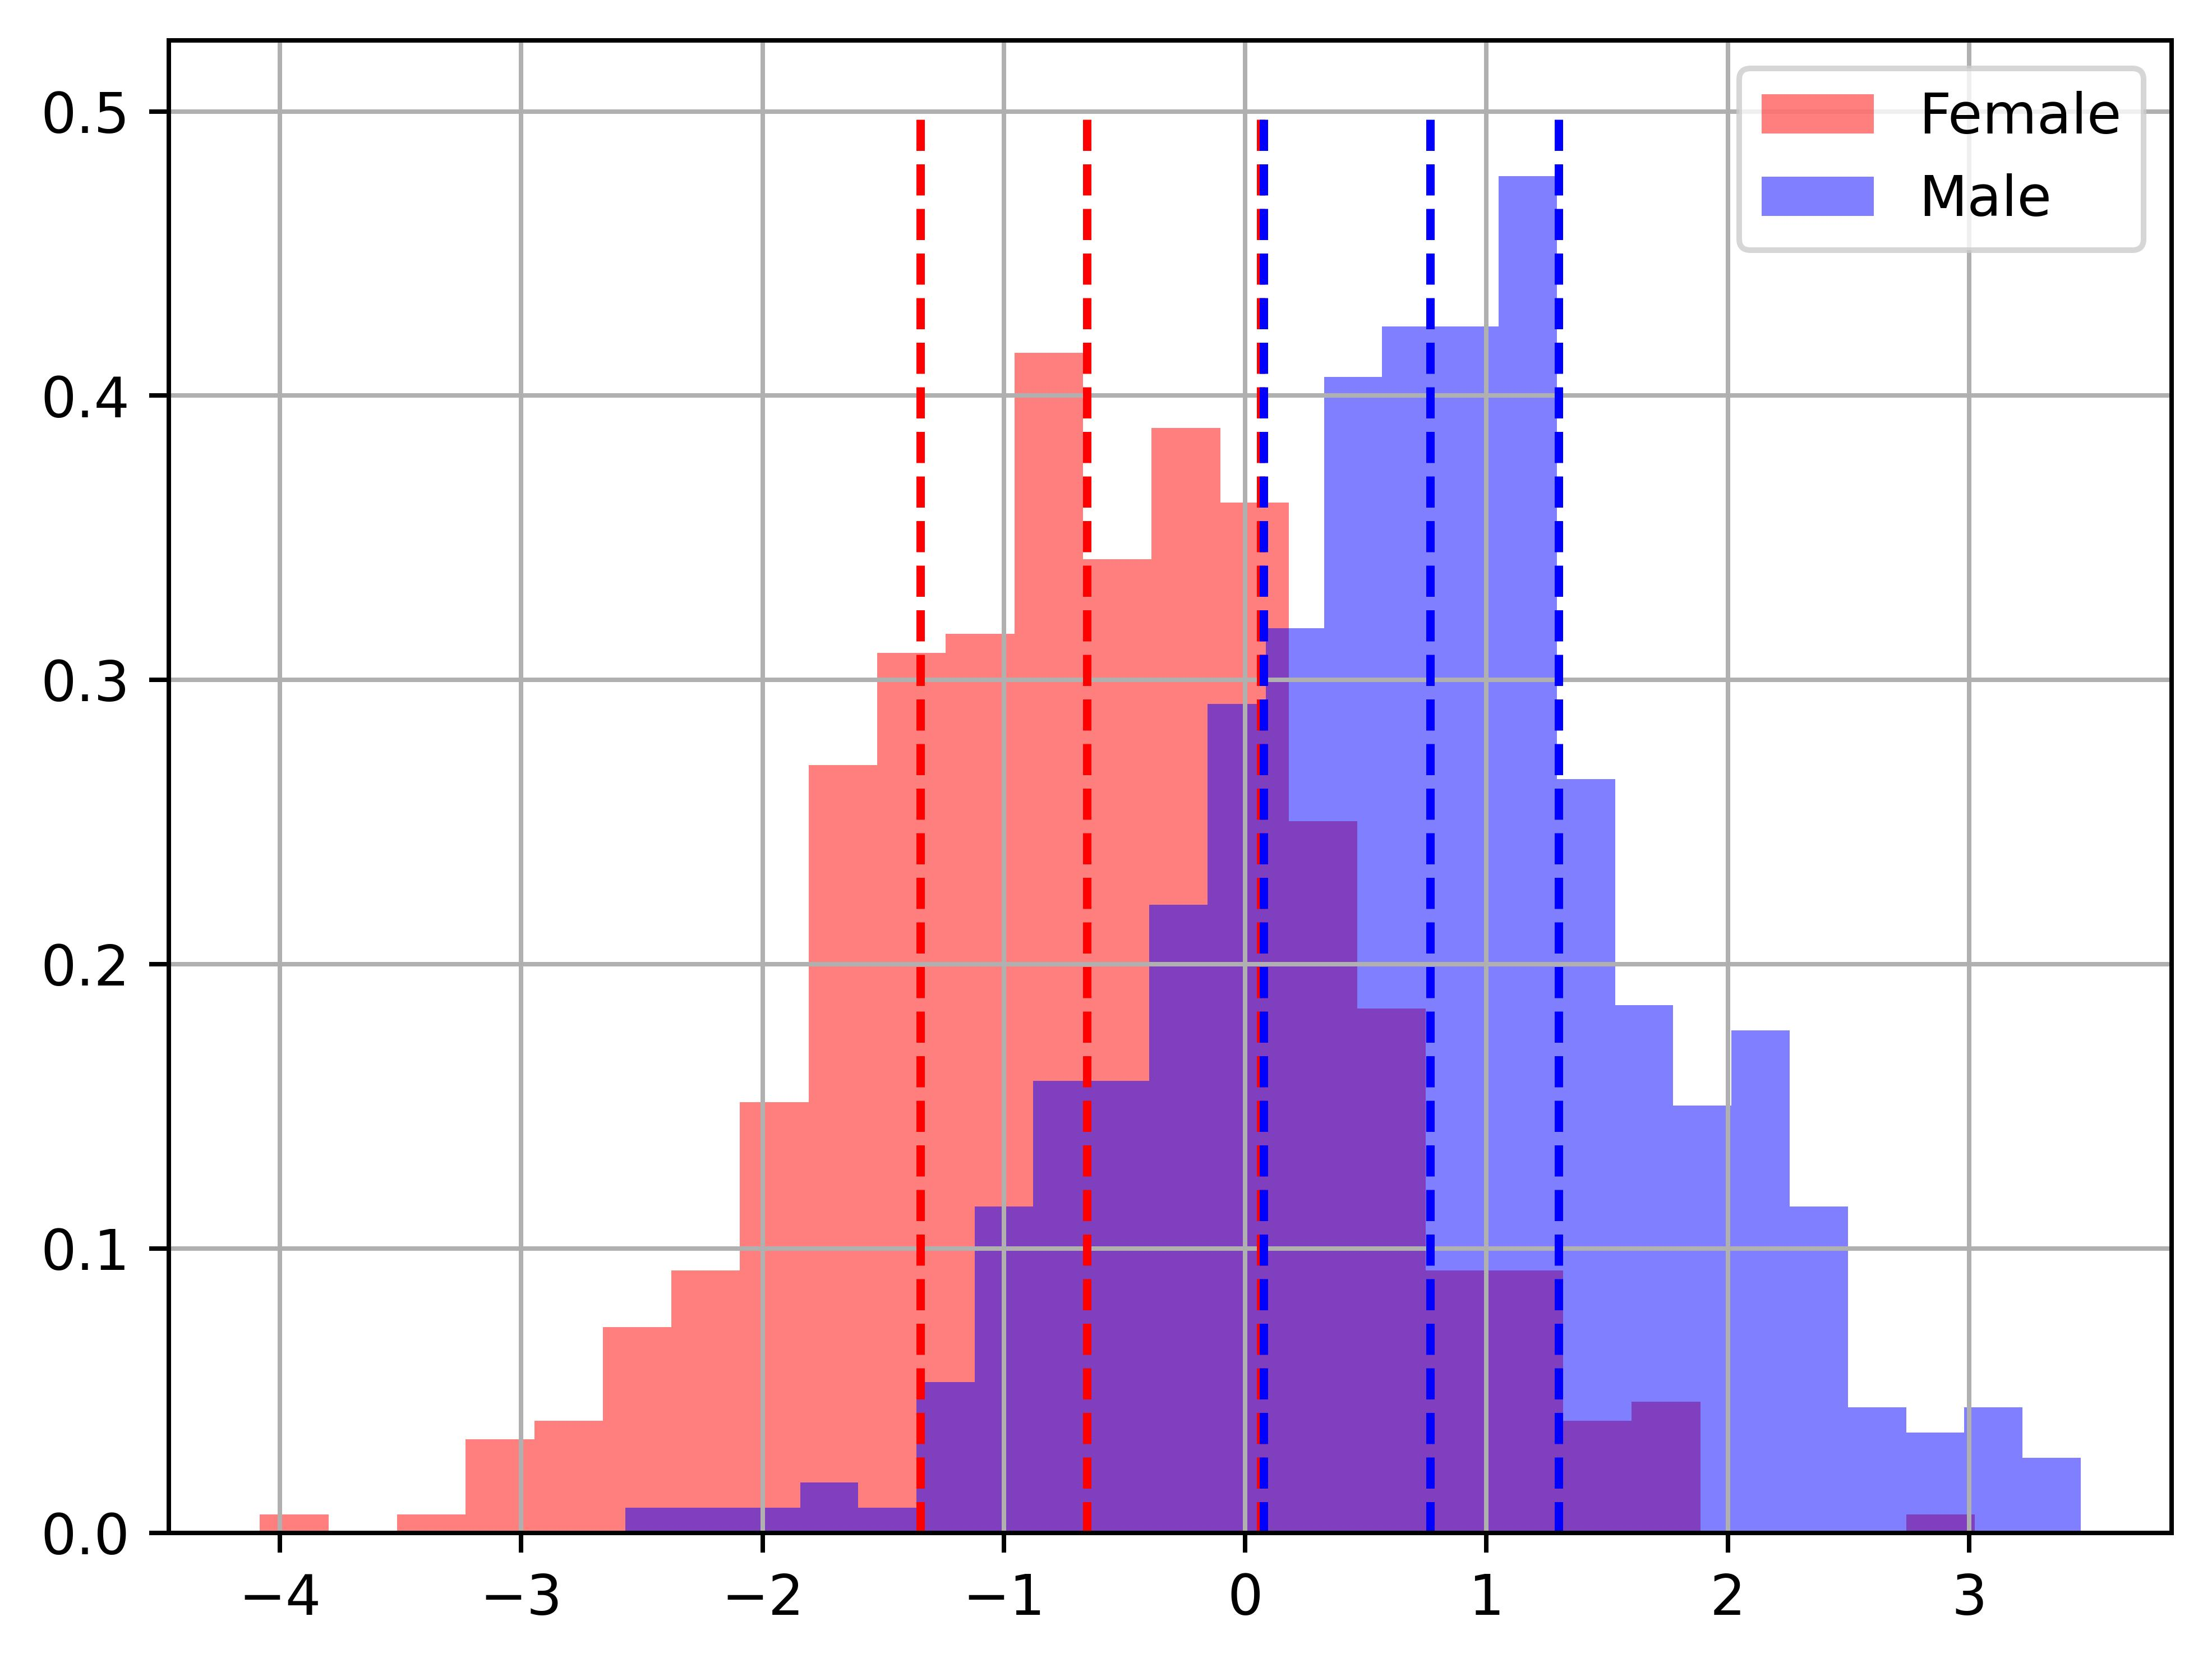
\includegraphics[width=0.4\textwidth]{../Analysis/LDA/node=15_size=480_step=180_rho=0.1/hist_2.jpg}}
    \subfloat[]{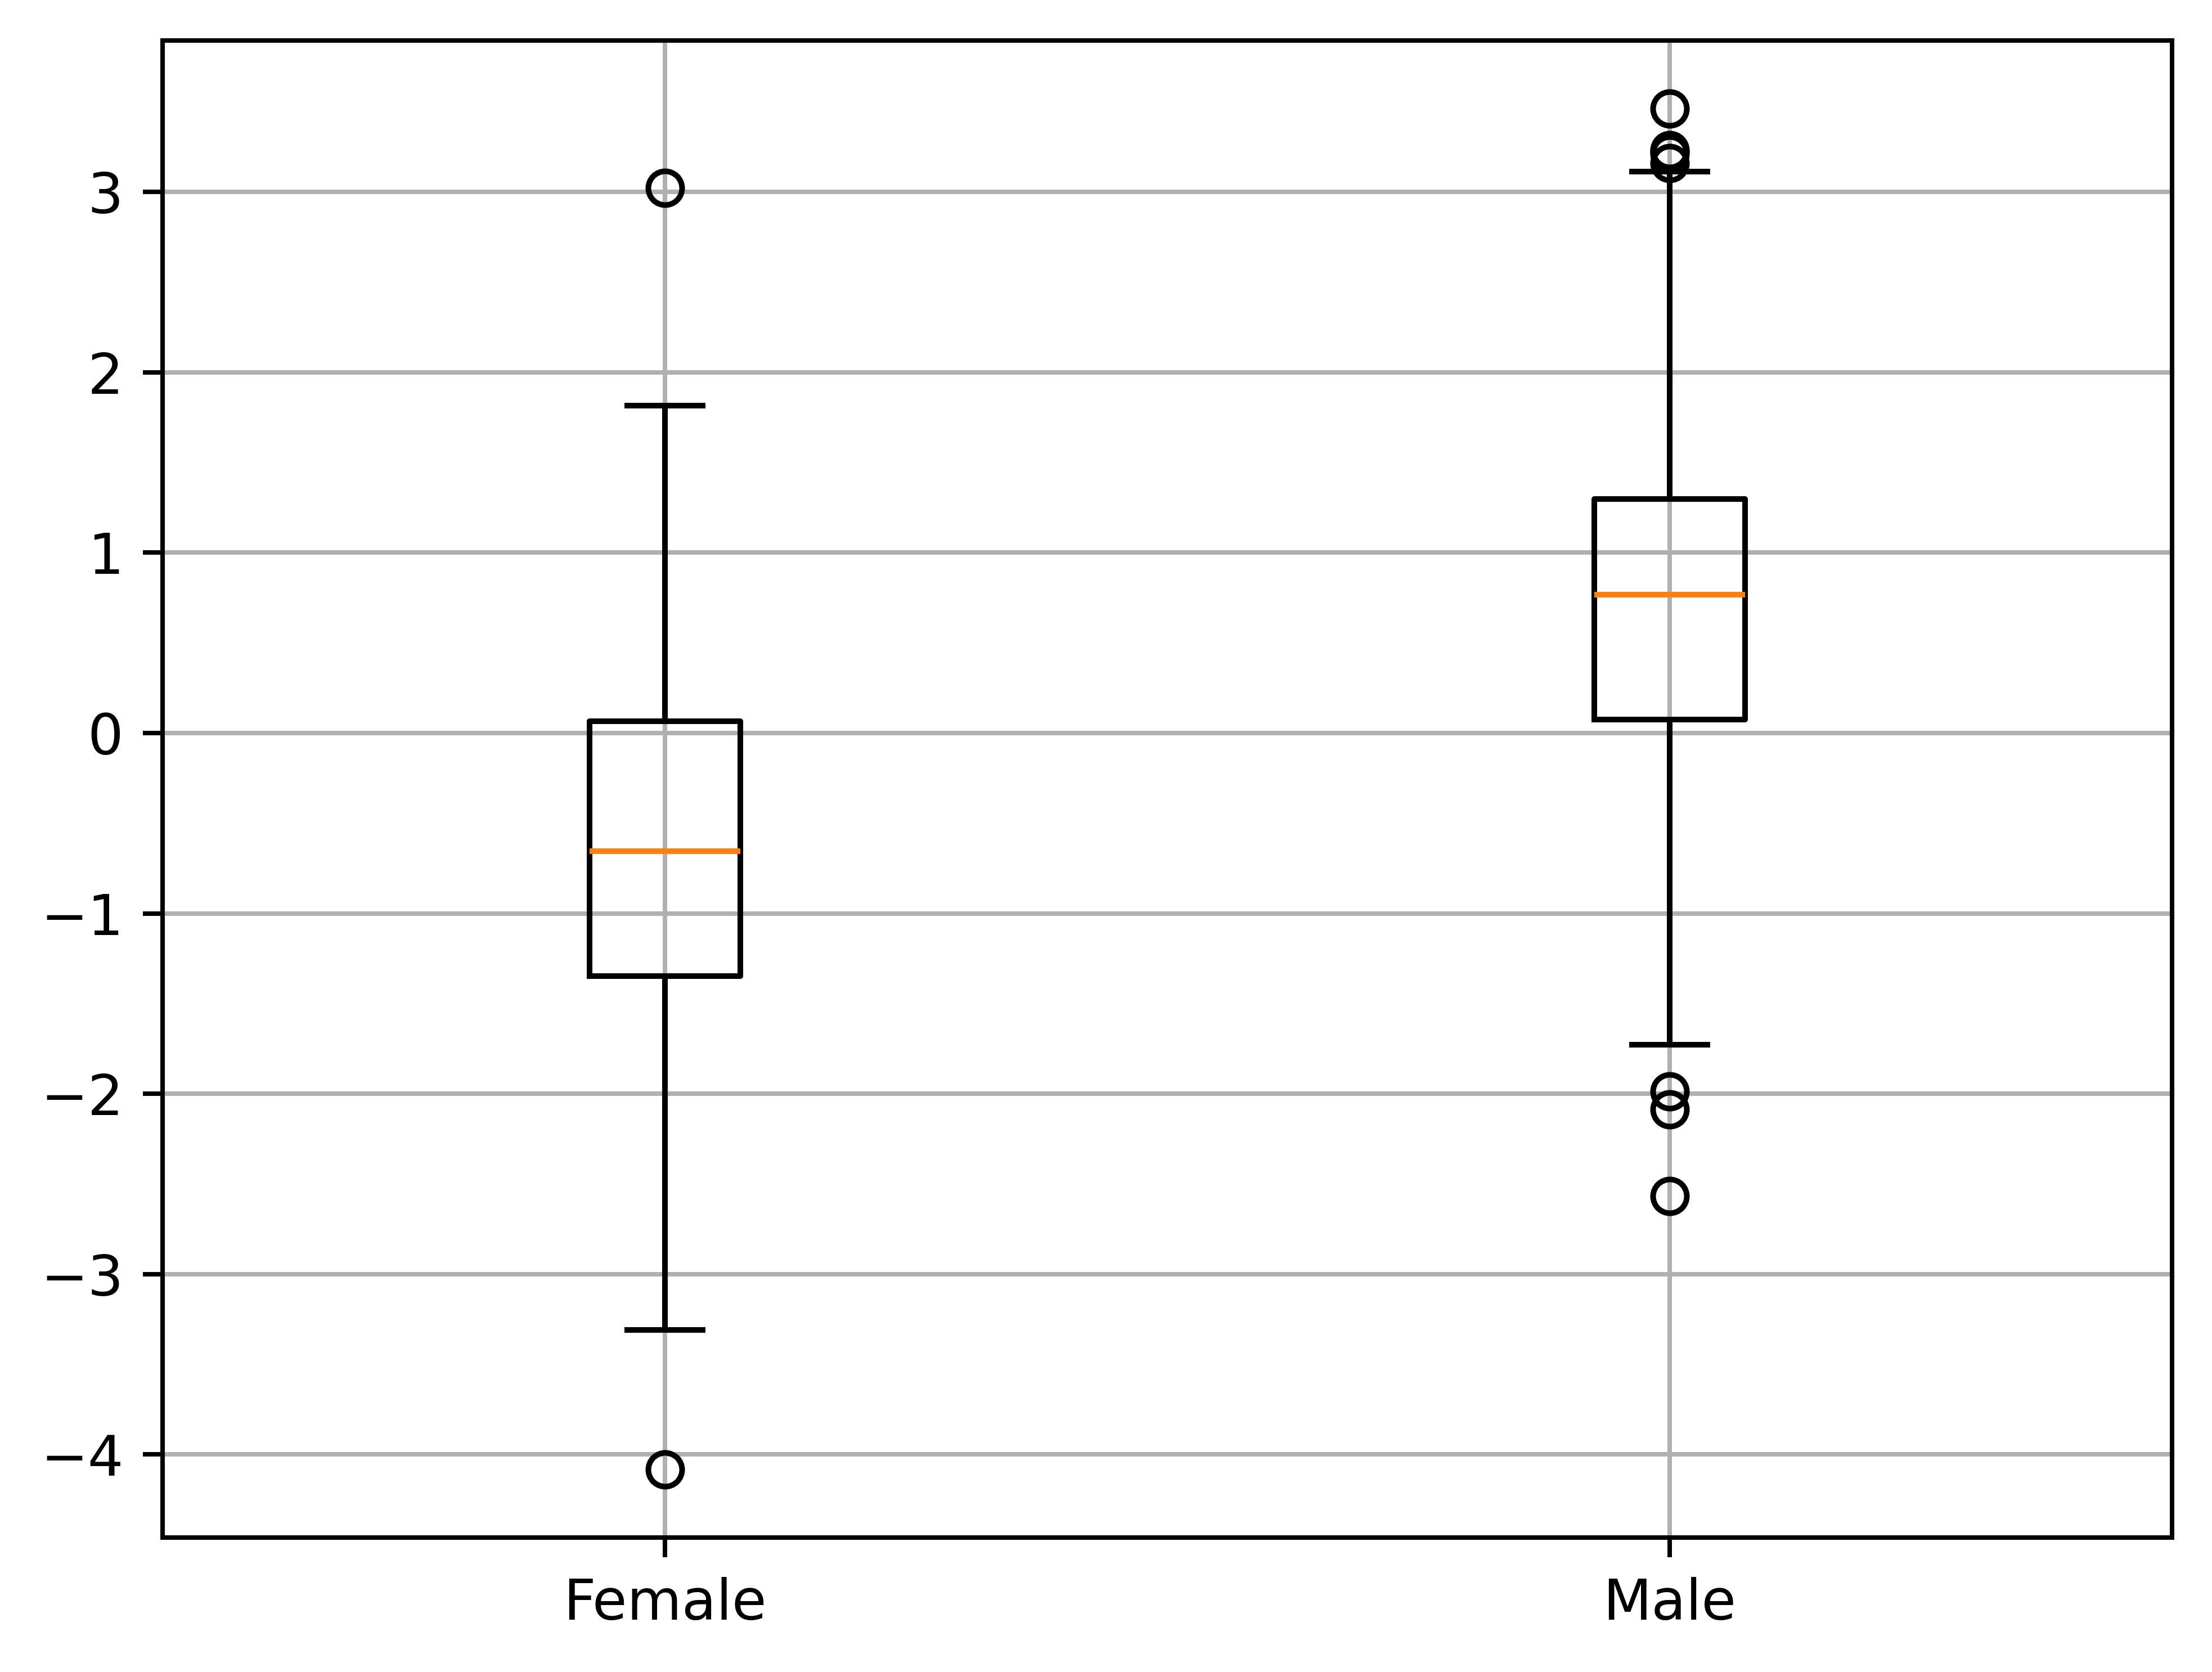
\includegraphics[width=0.4\textwidth]{../Analysis/LDA/node=15_size=480_step=180_rho=0.1/box_2.jpg}} \\
    \caption{LDA for Dynamic connectivity with $N_{node} = 15$.}
    \label{LDA-example-2}
\end{figure}

\begin{figure}[H]
    \centering
    \subfloat[]{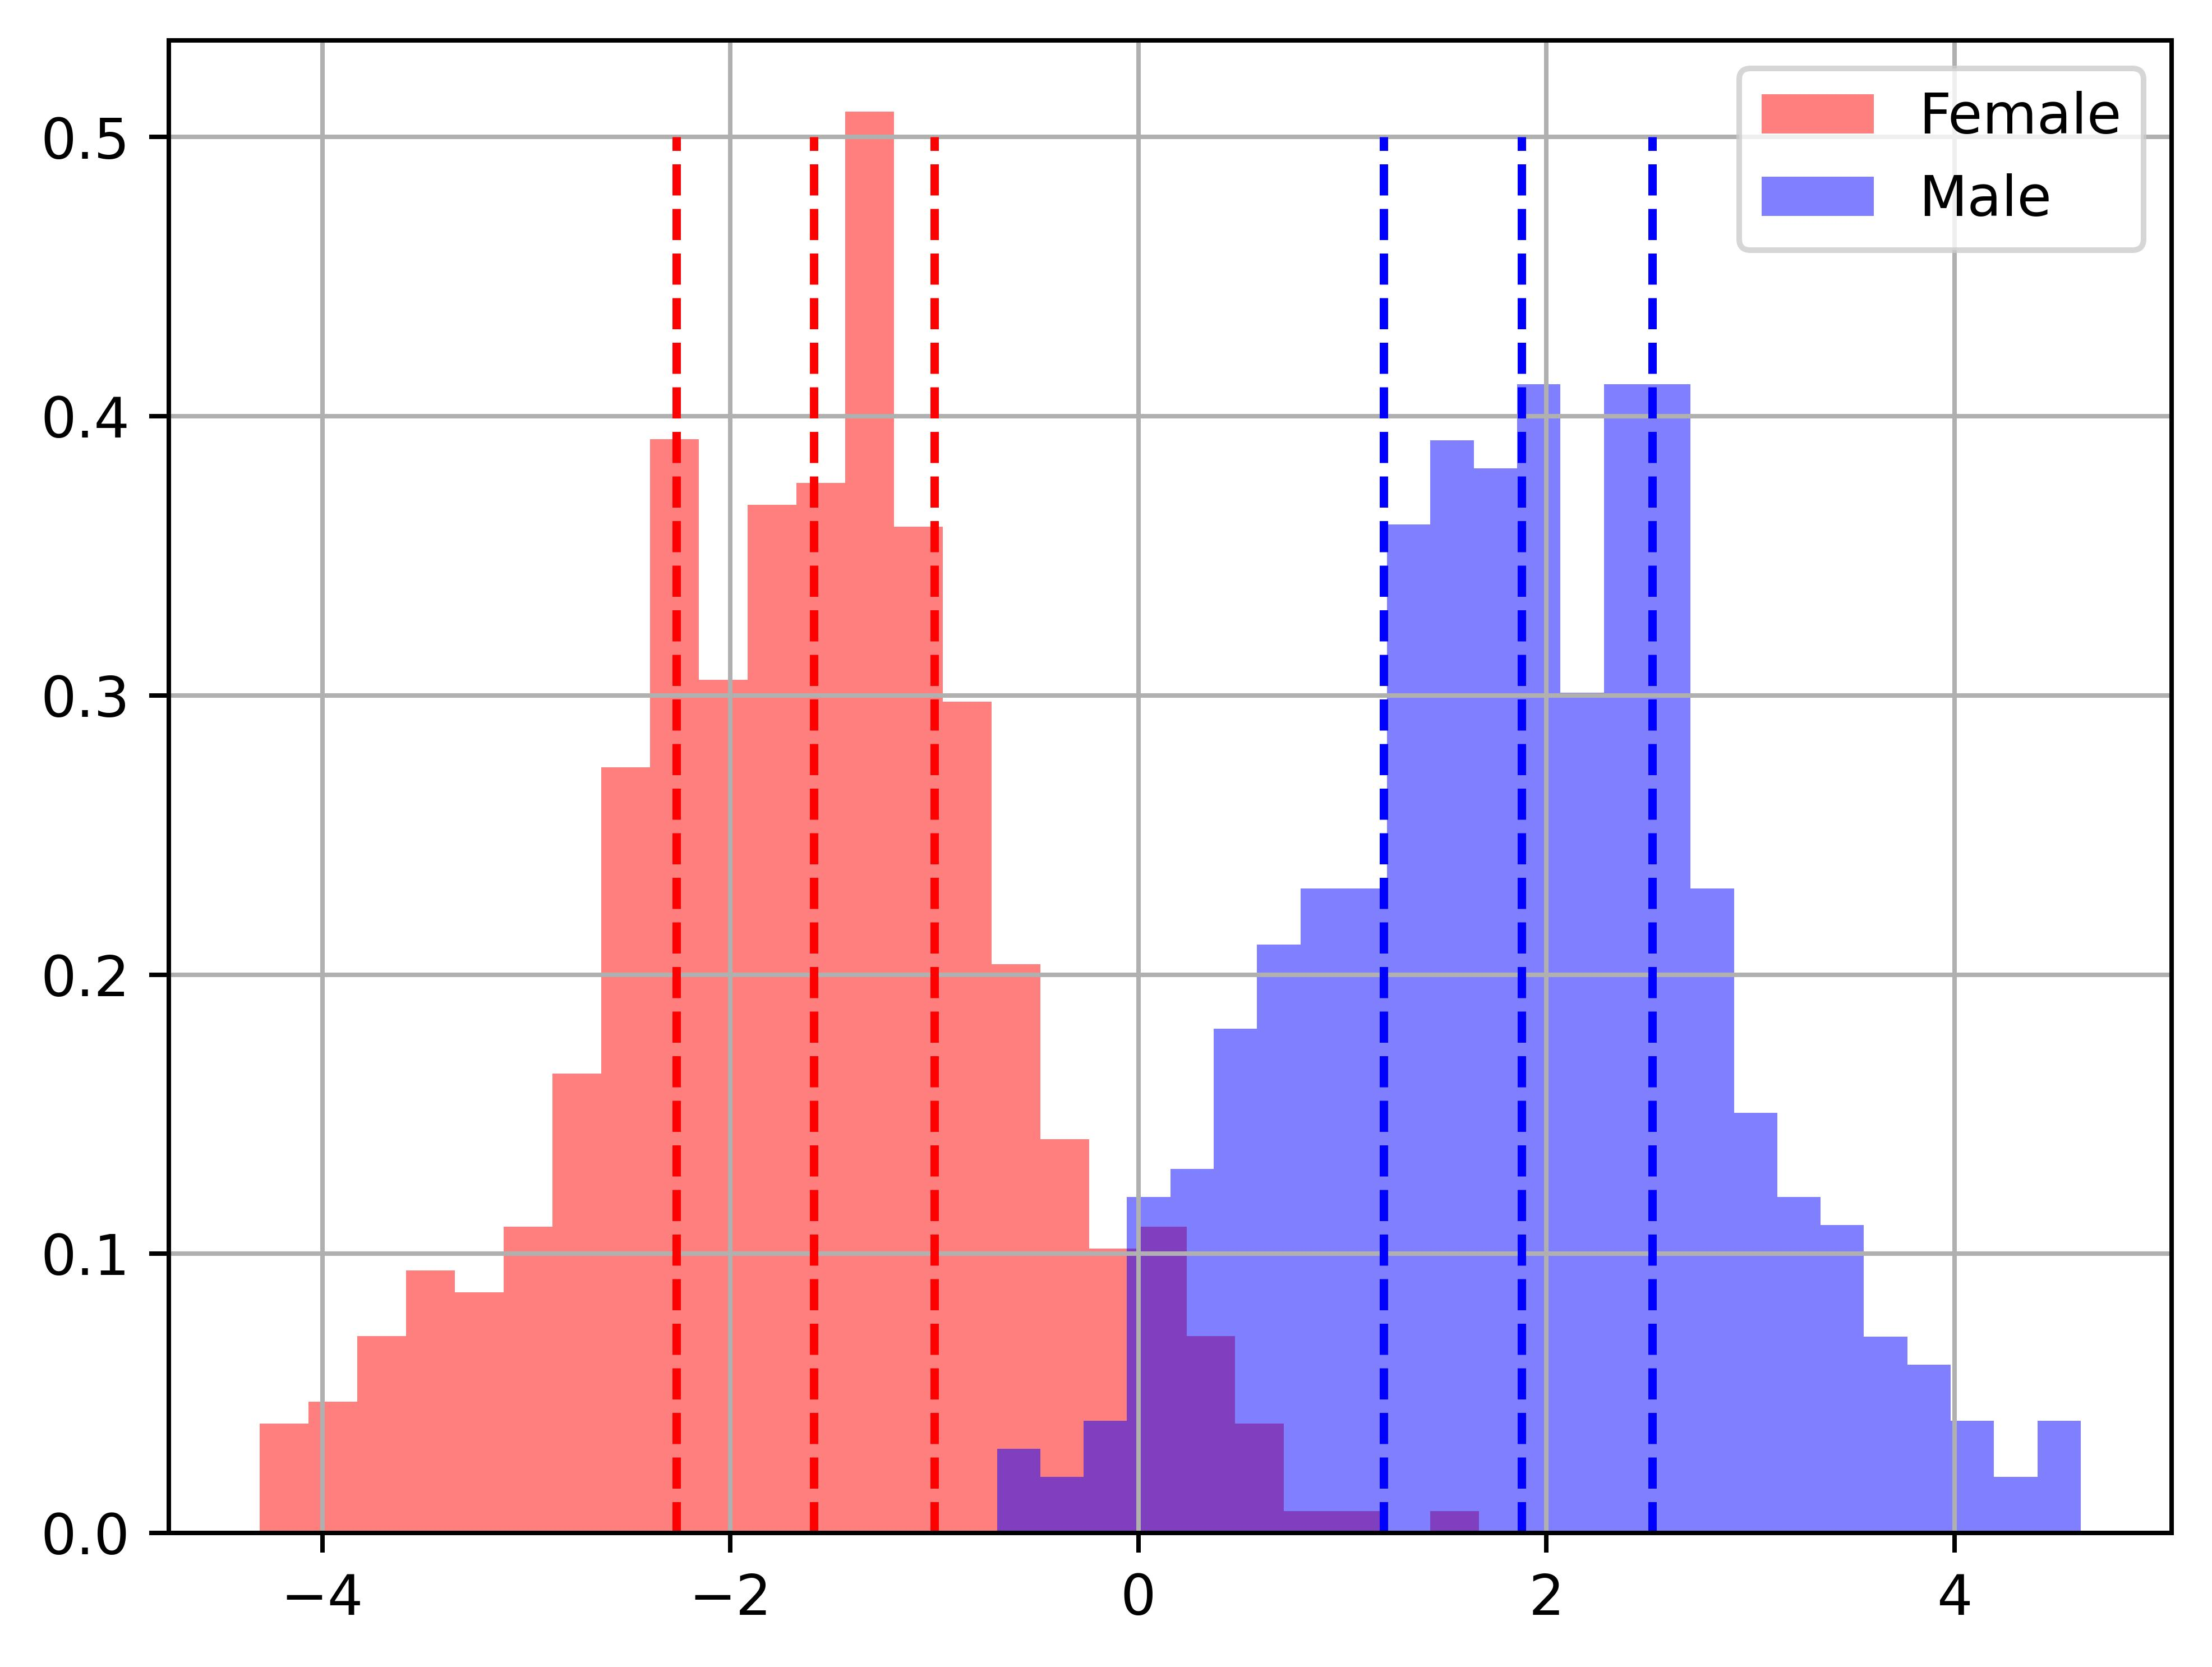
\includegraphics[width=0.4\textwidth]{../Analysis/LDA/node=25_size=4800_step=4800_rho=0.1/hist_0.jpg}}
    \subfloat[]{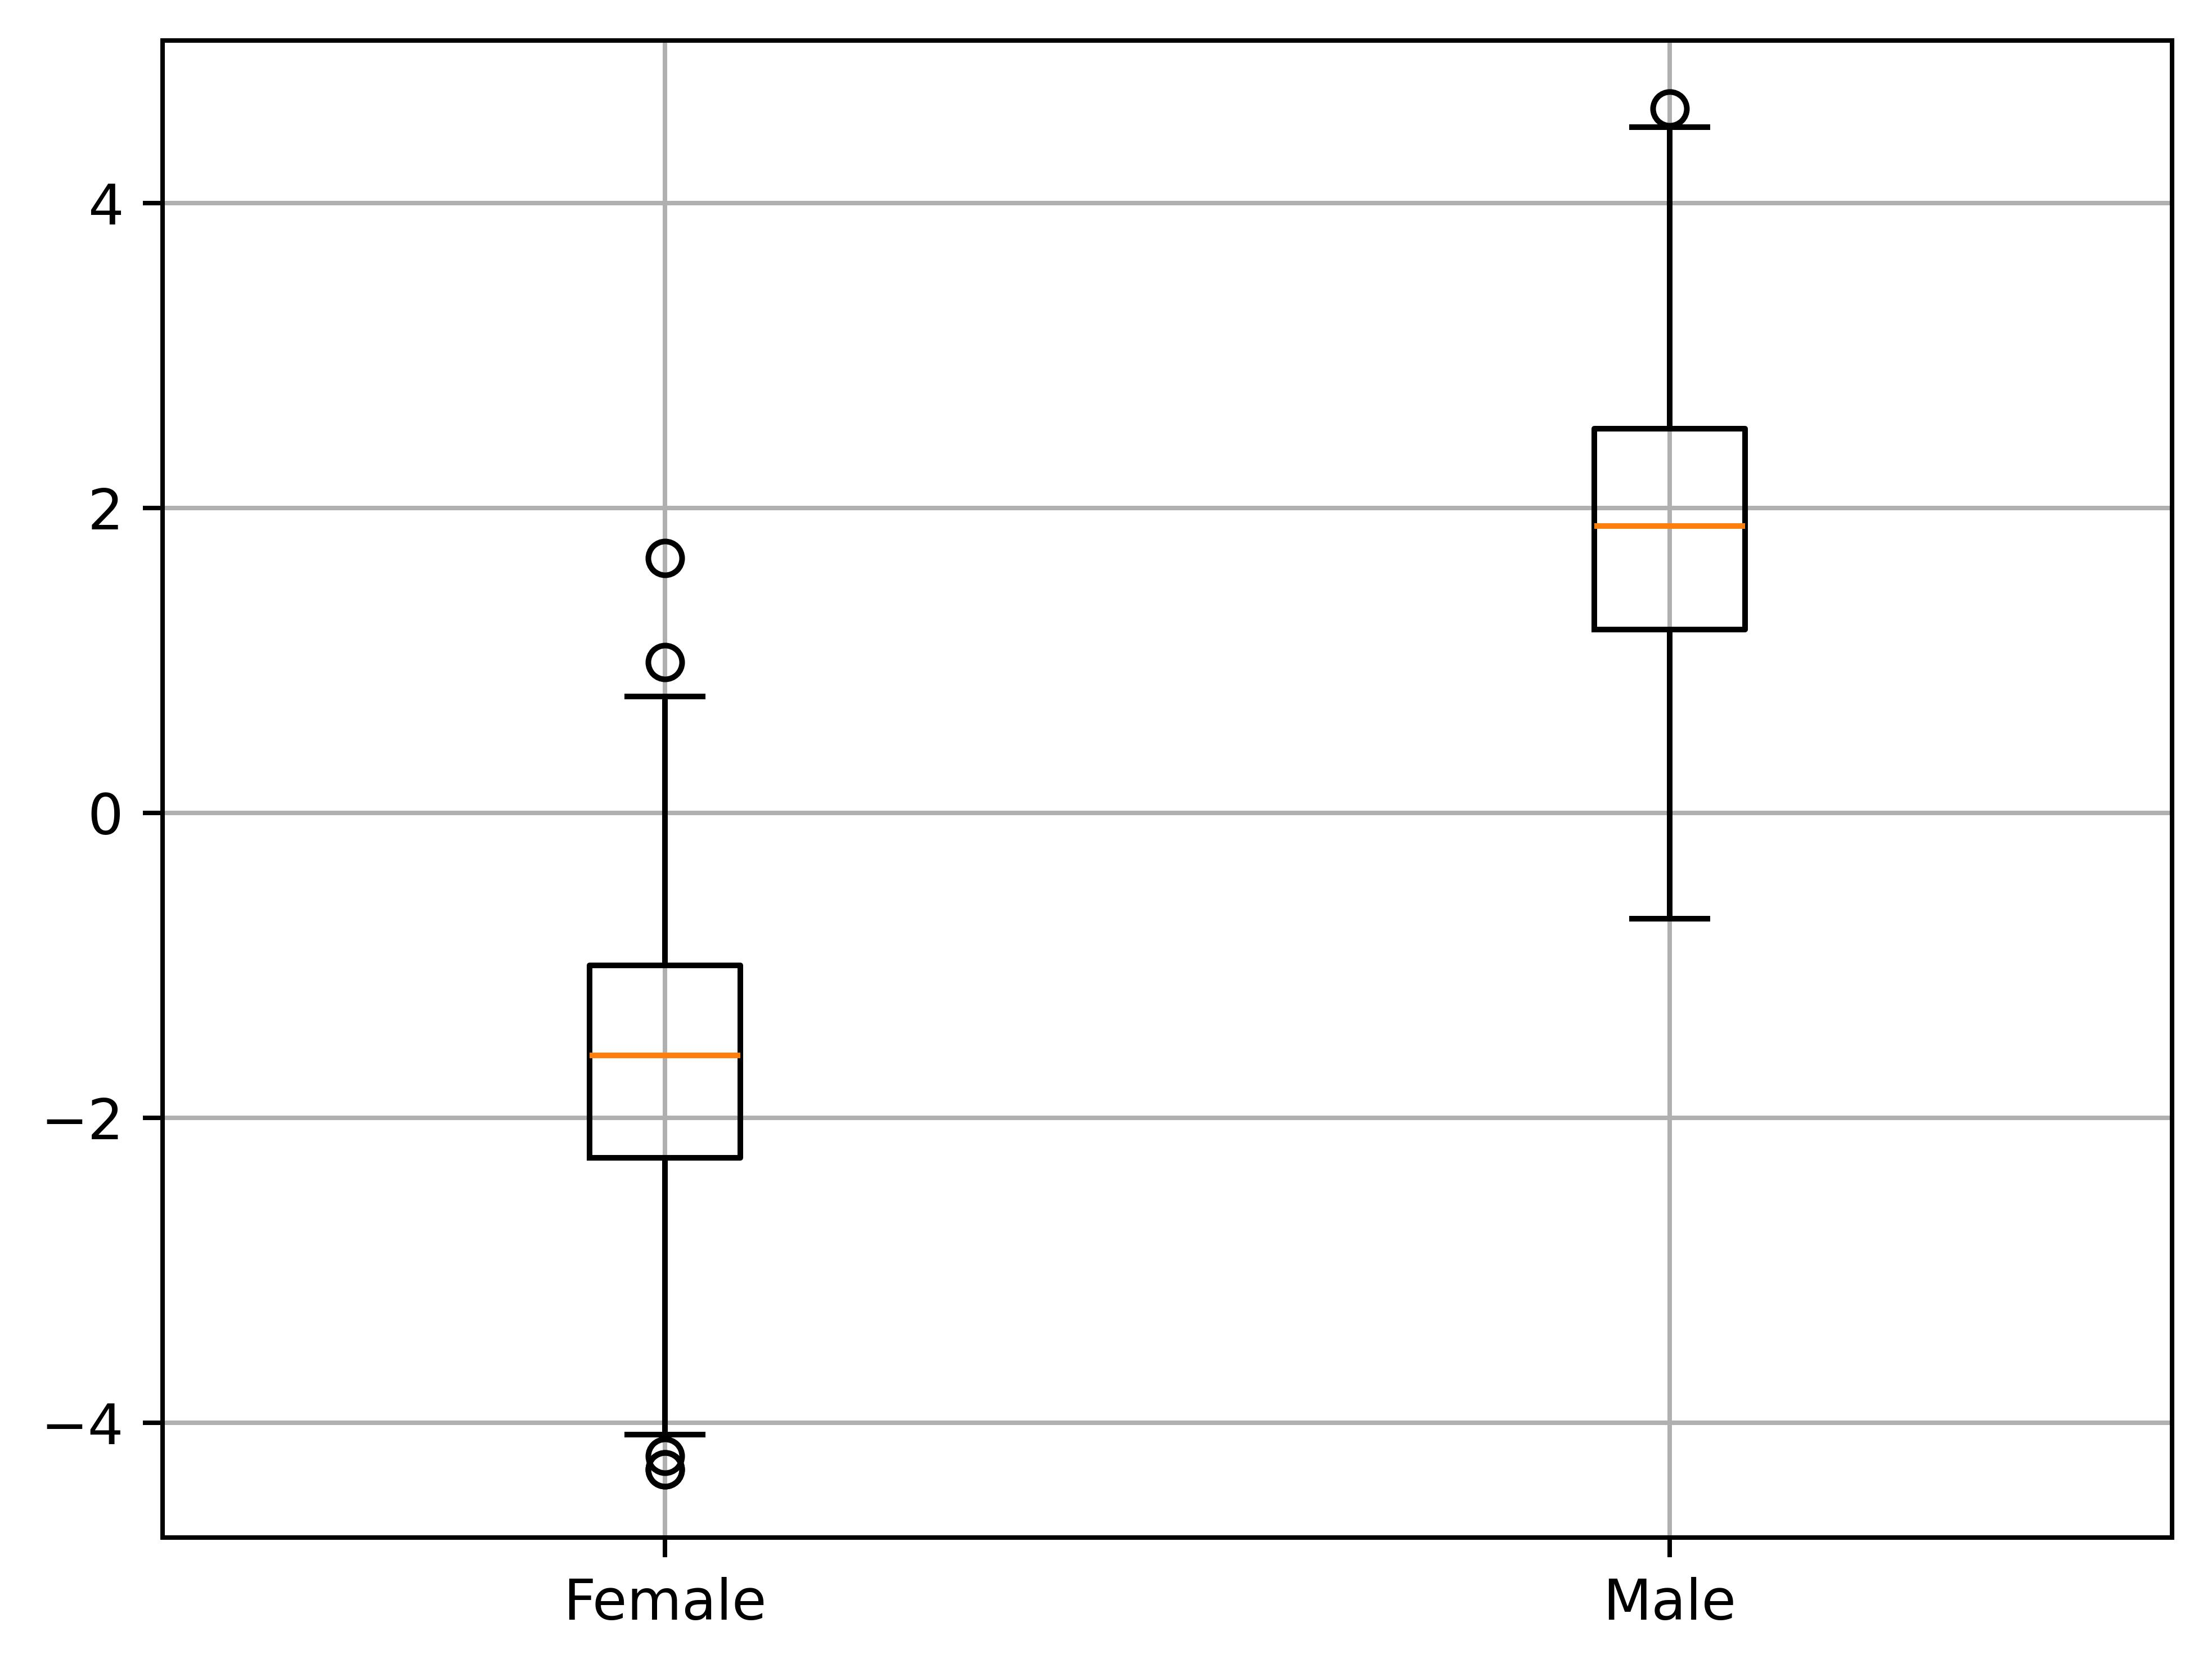
\includegraphics[width=0.4\textwidth]{../Analysis/LDA/node=25_size=4800_step=4800_rho=0.1/box_0.jpg}} \\
    \caption{LDA for static connectivity with $N_{node} = 25$.}
    \label{LDA-example-3}
\end{figure}

\begin{figure}[H]
    \centering
    \subfloat[]{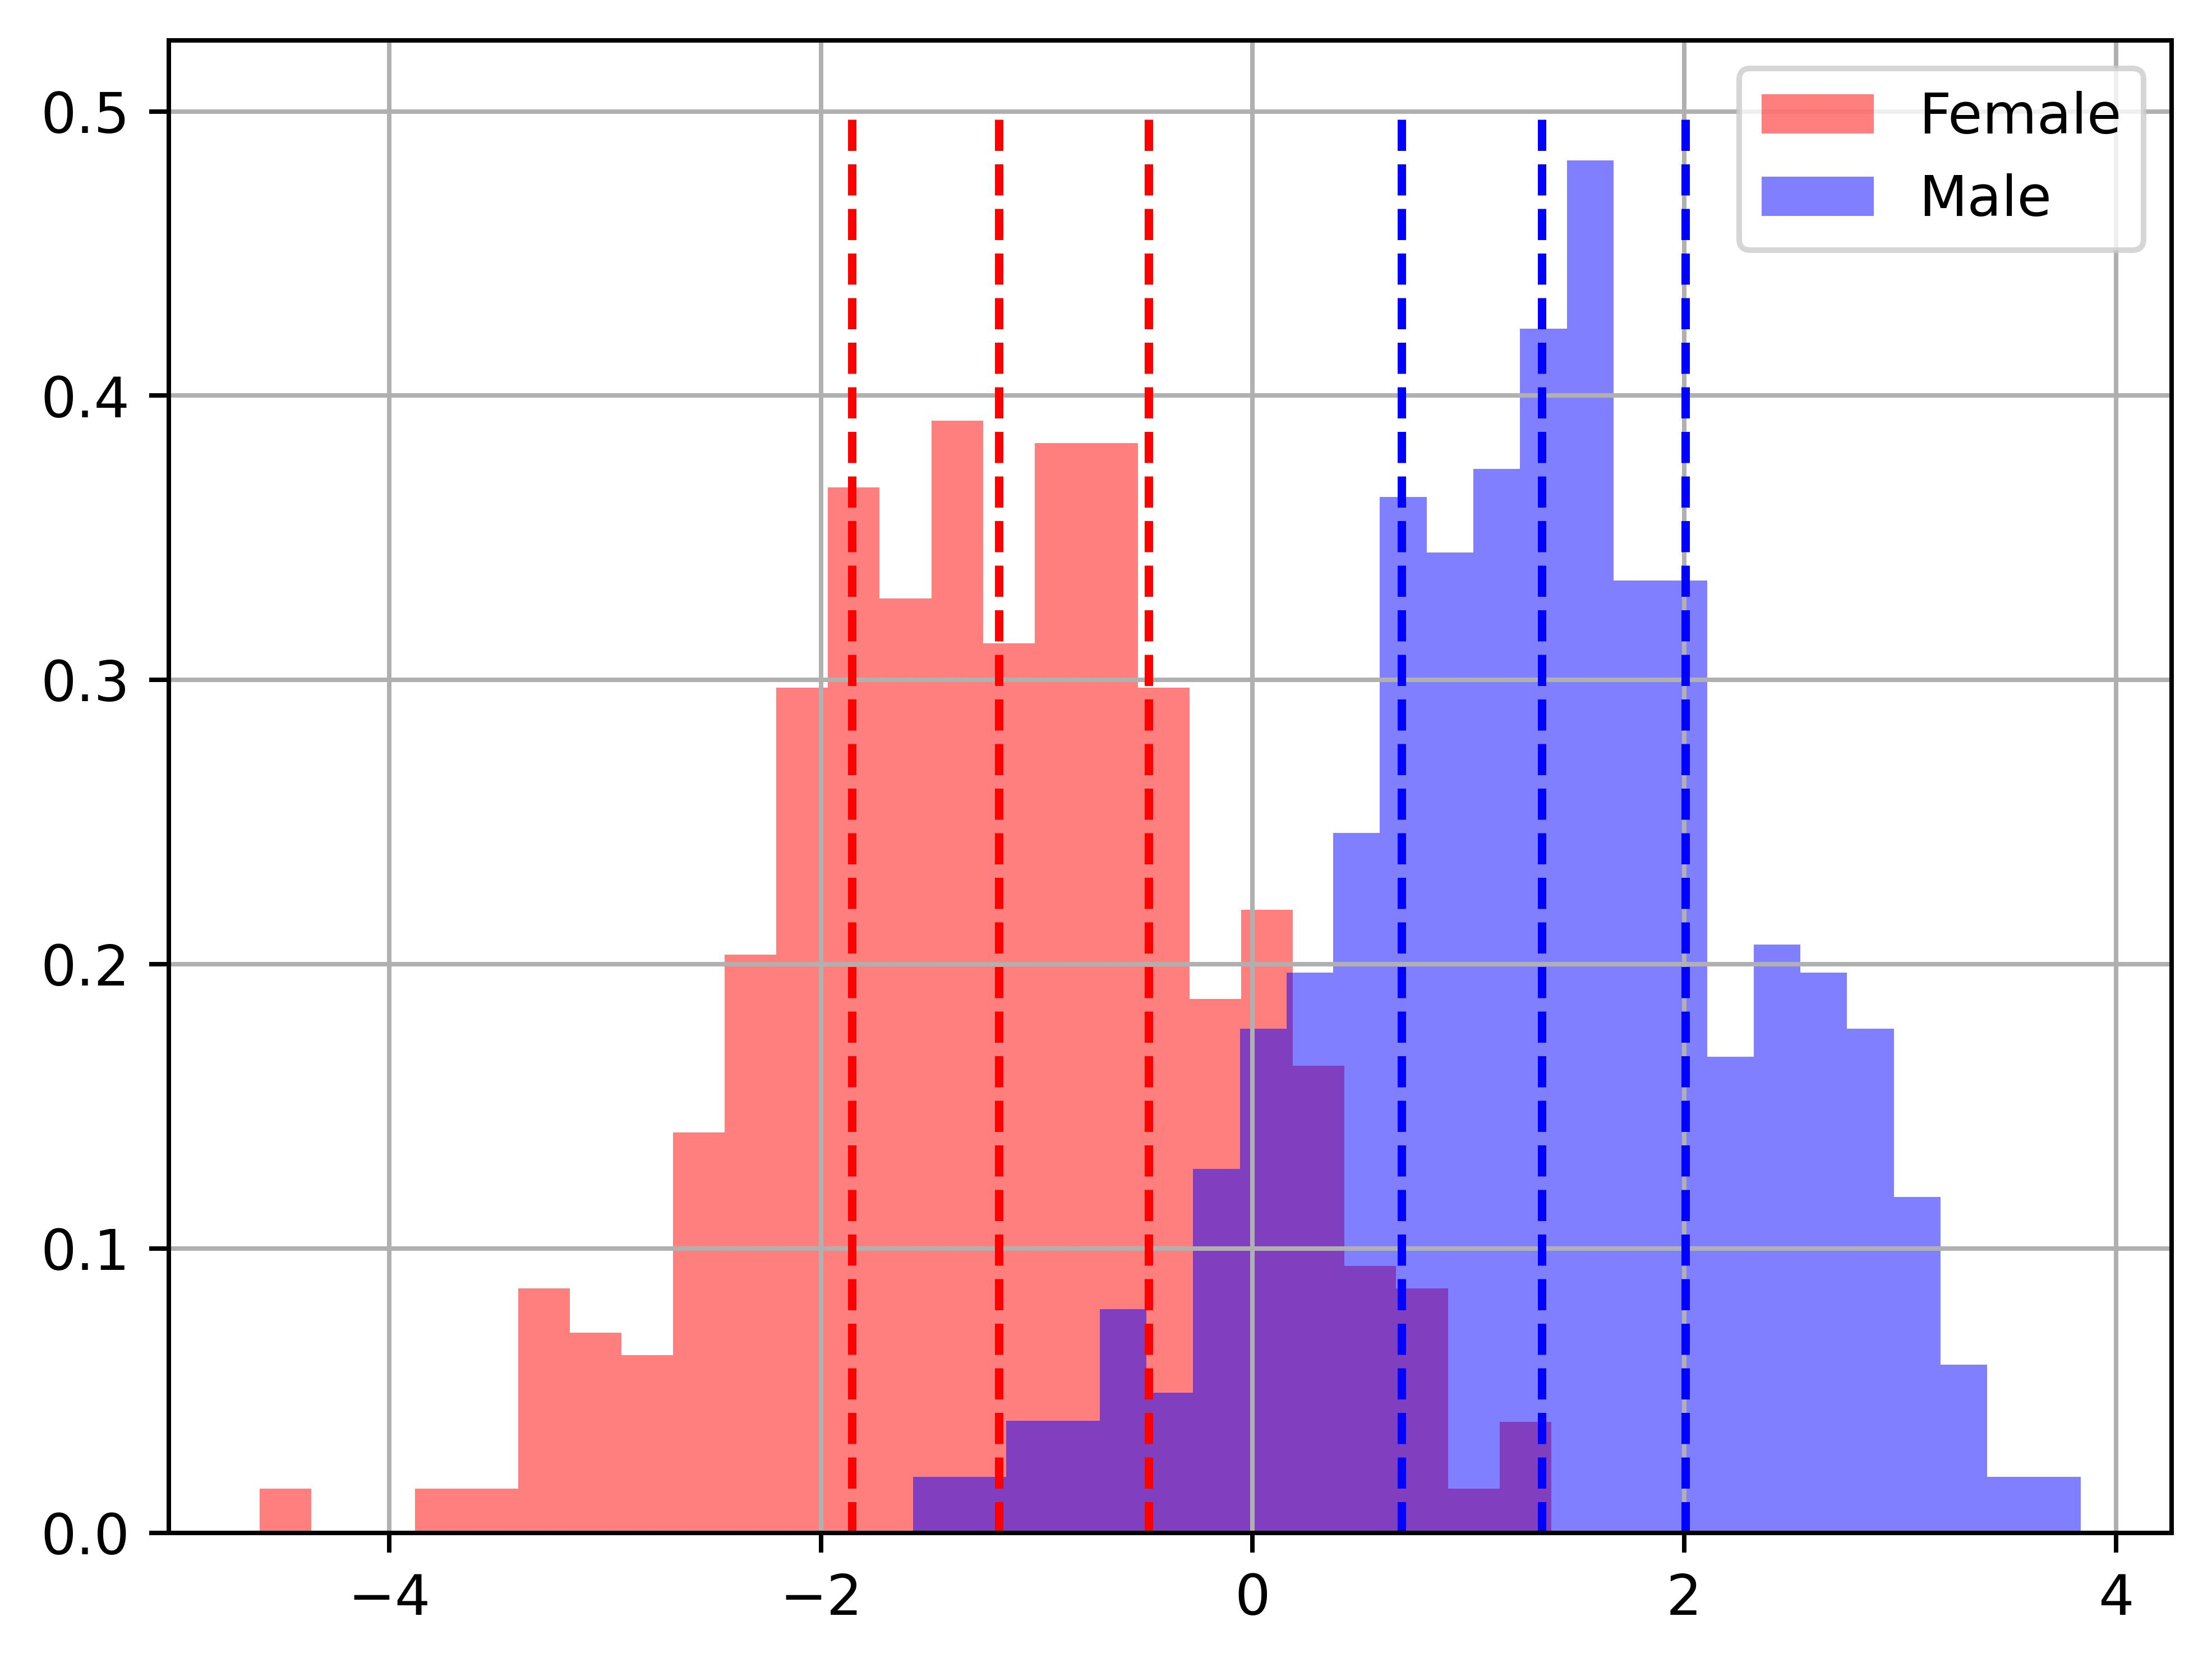
\includegraphics[width=0.4\textwidth]{../Analysis/LDA/node=25_size=480_step=180_rho=0.1/hist_0.jpg}}
    \subfloat[]{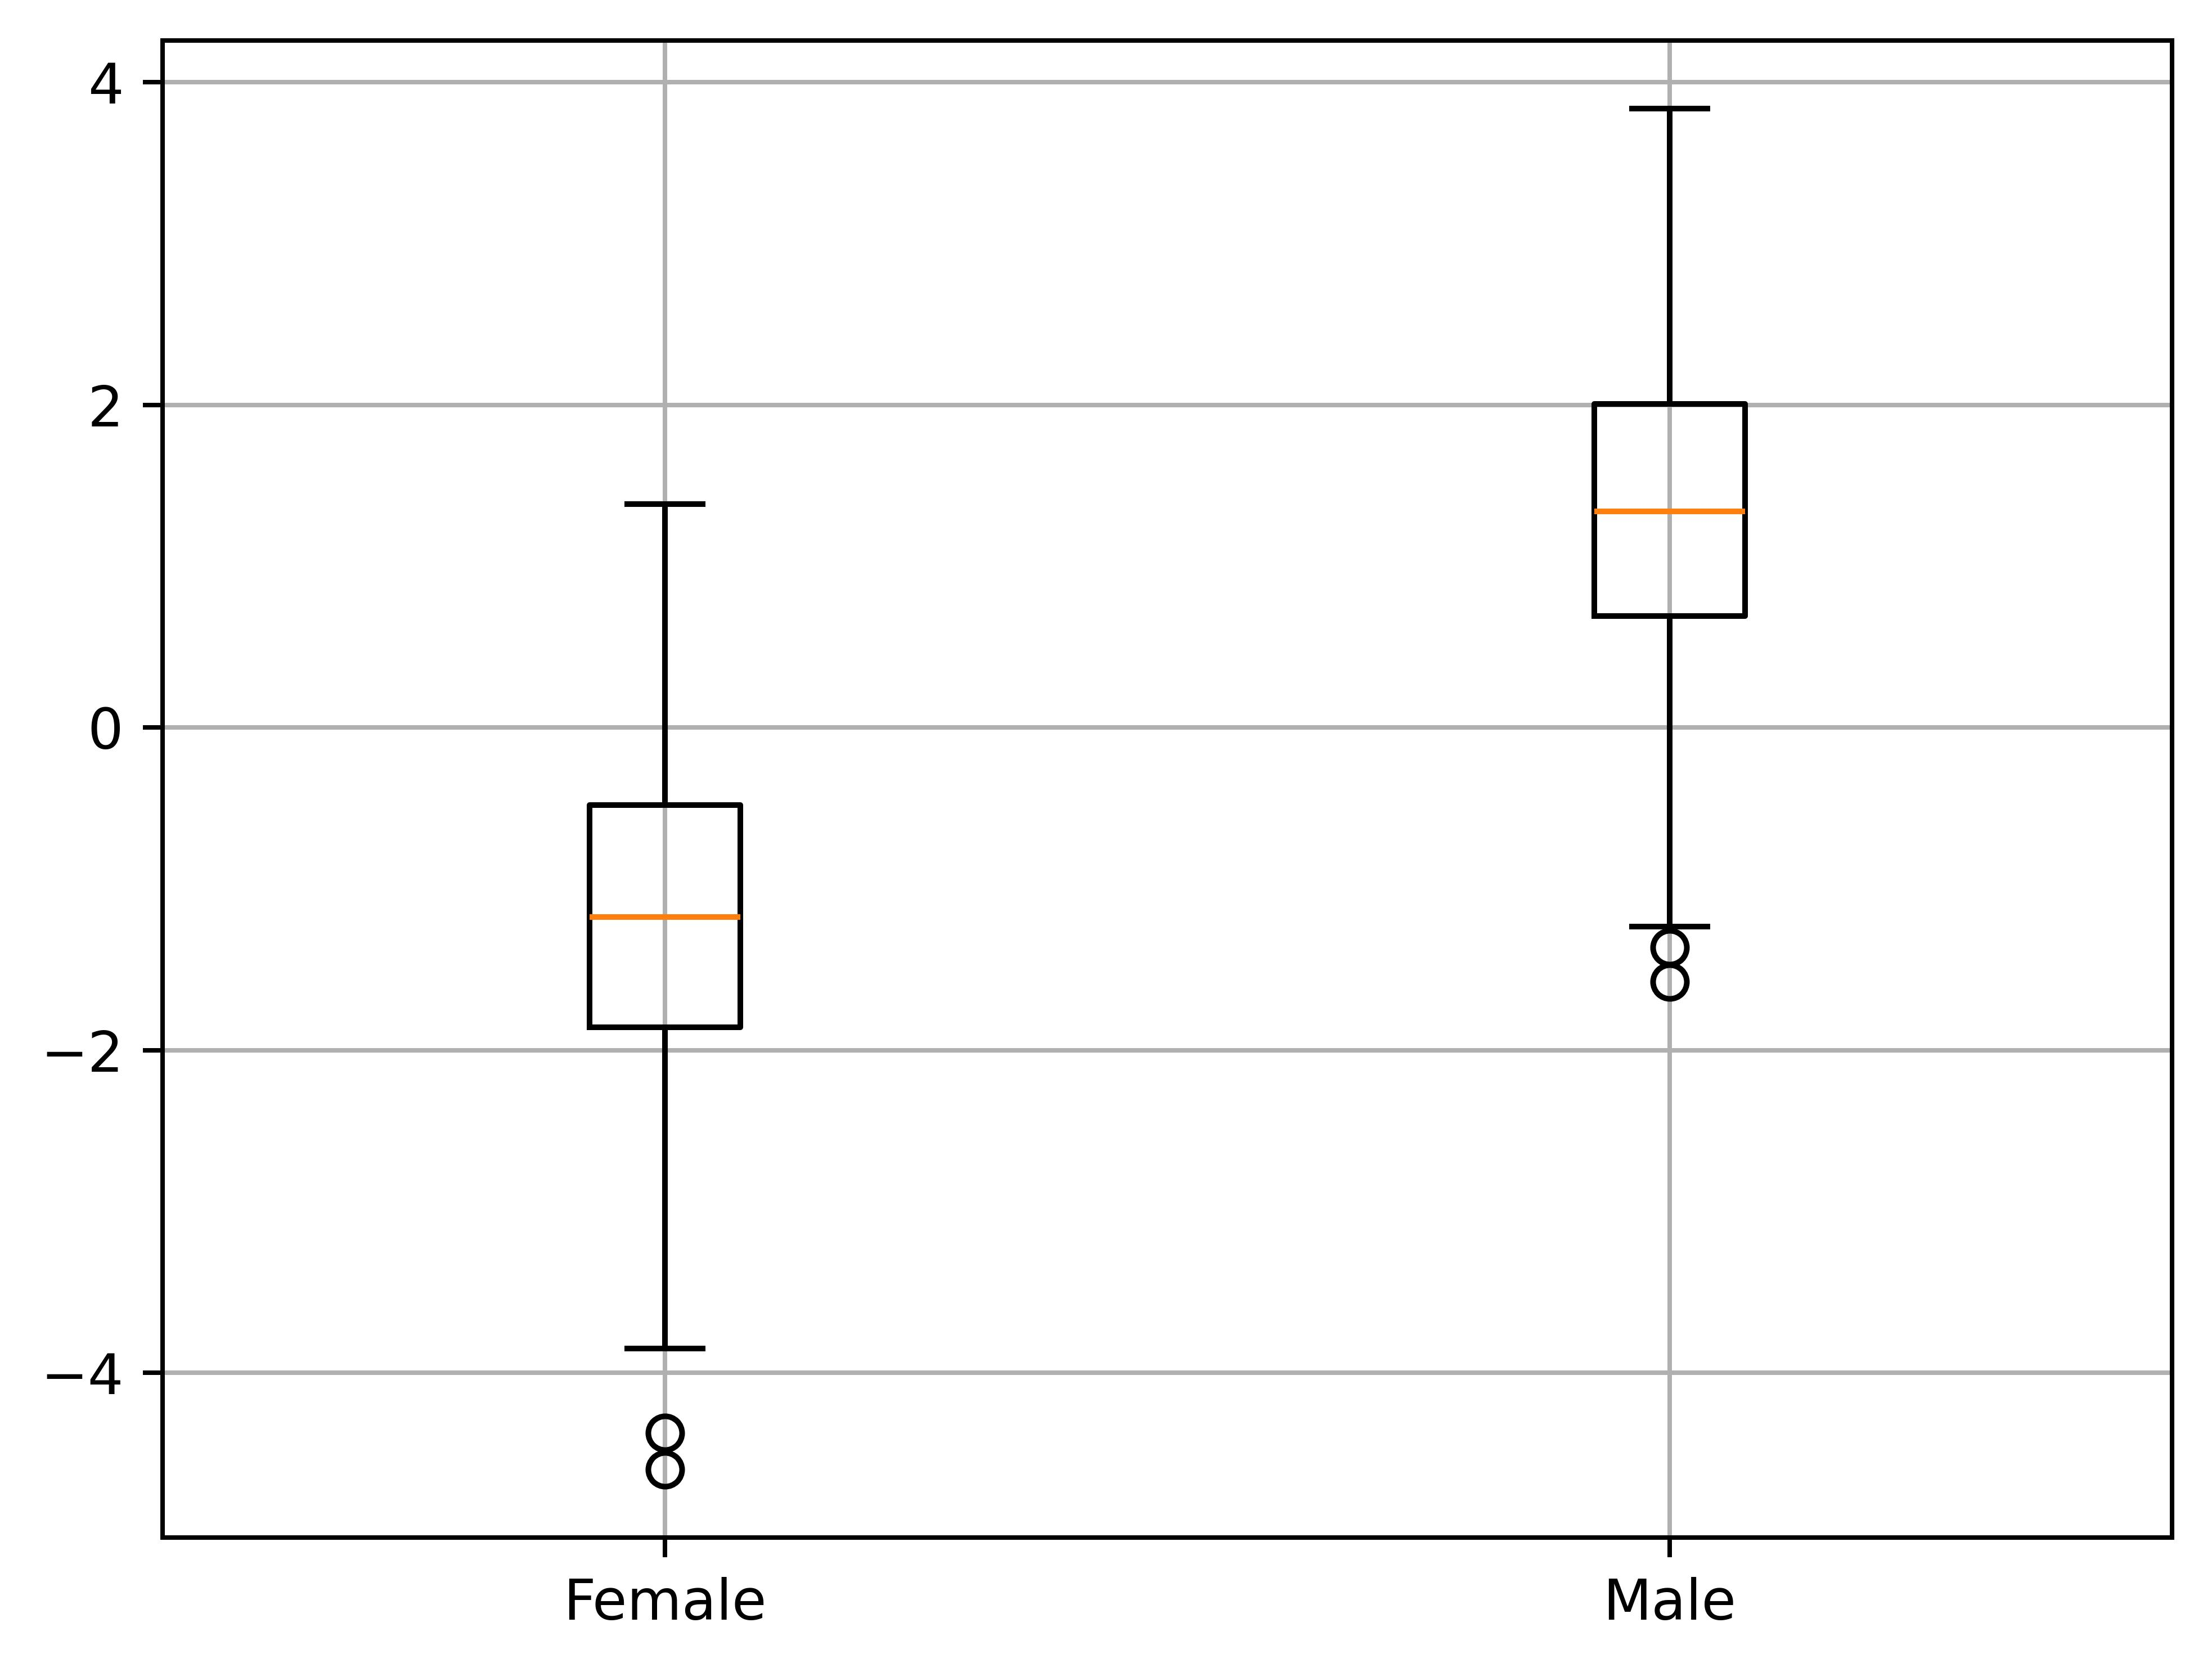
\includegraphics[width=0.4\textwidth]{../Analysis/LDA/node=25_size=480_step=180_rho=0.1/box_0.jpg}} \\
    \subfloat[]{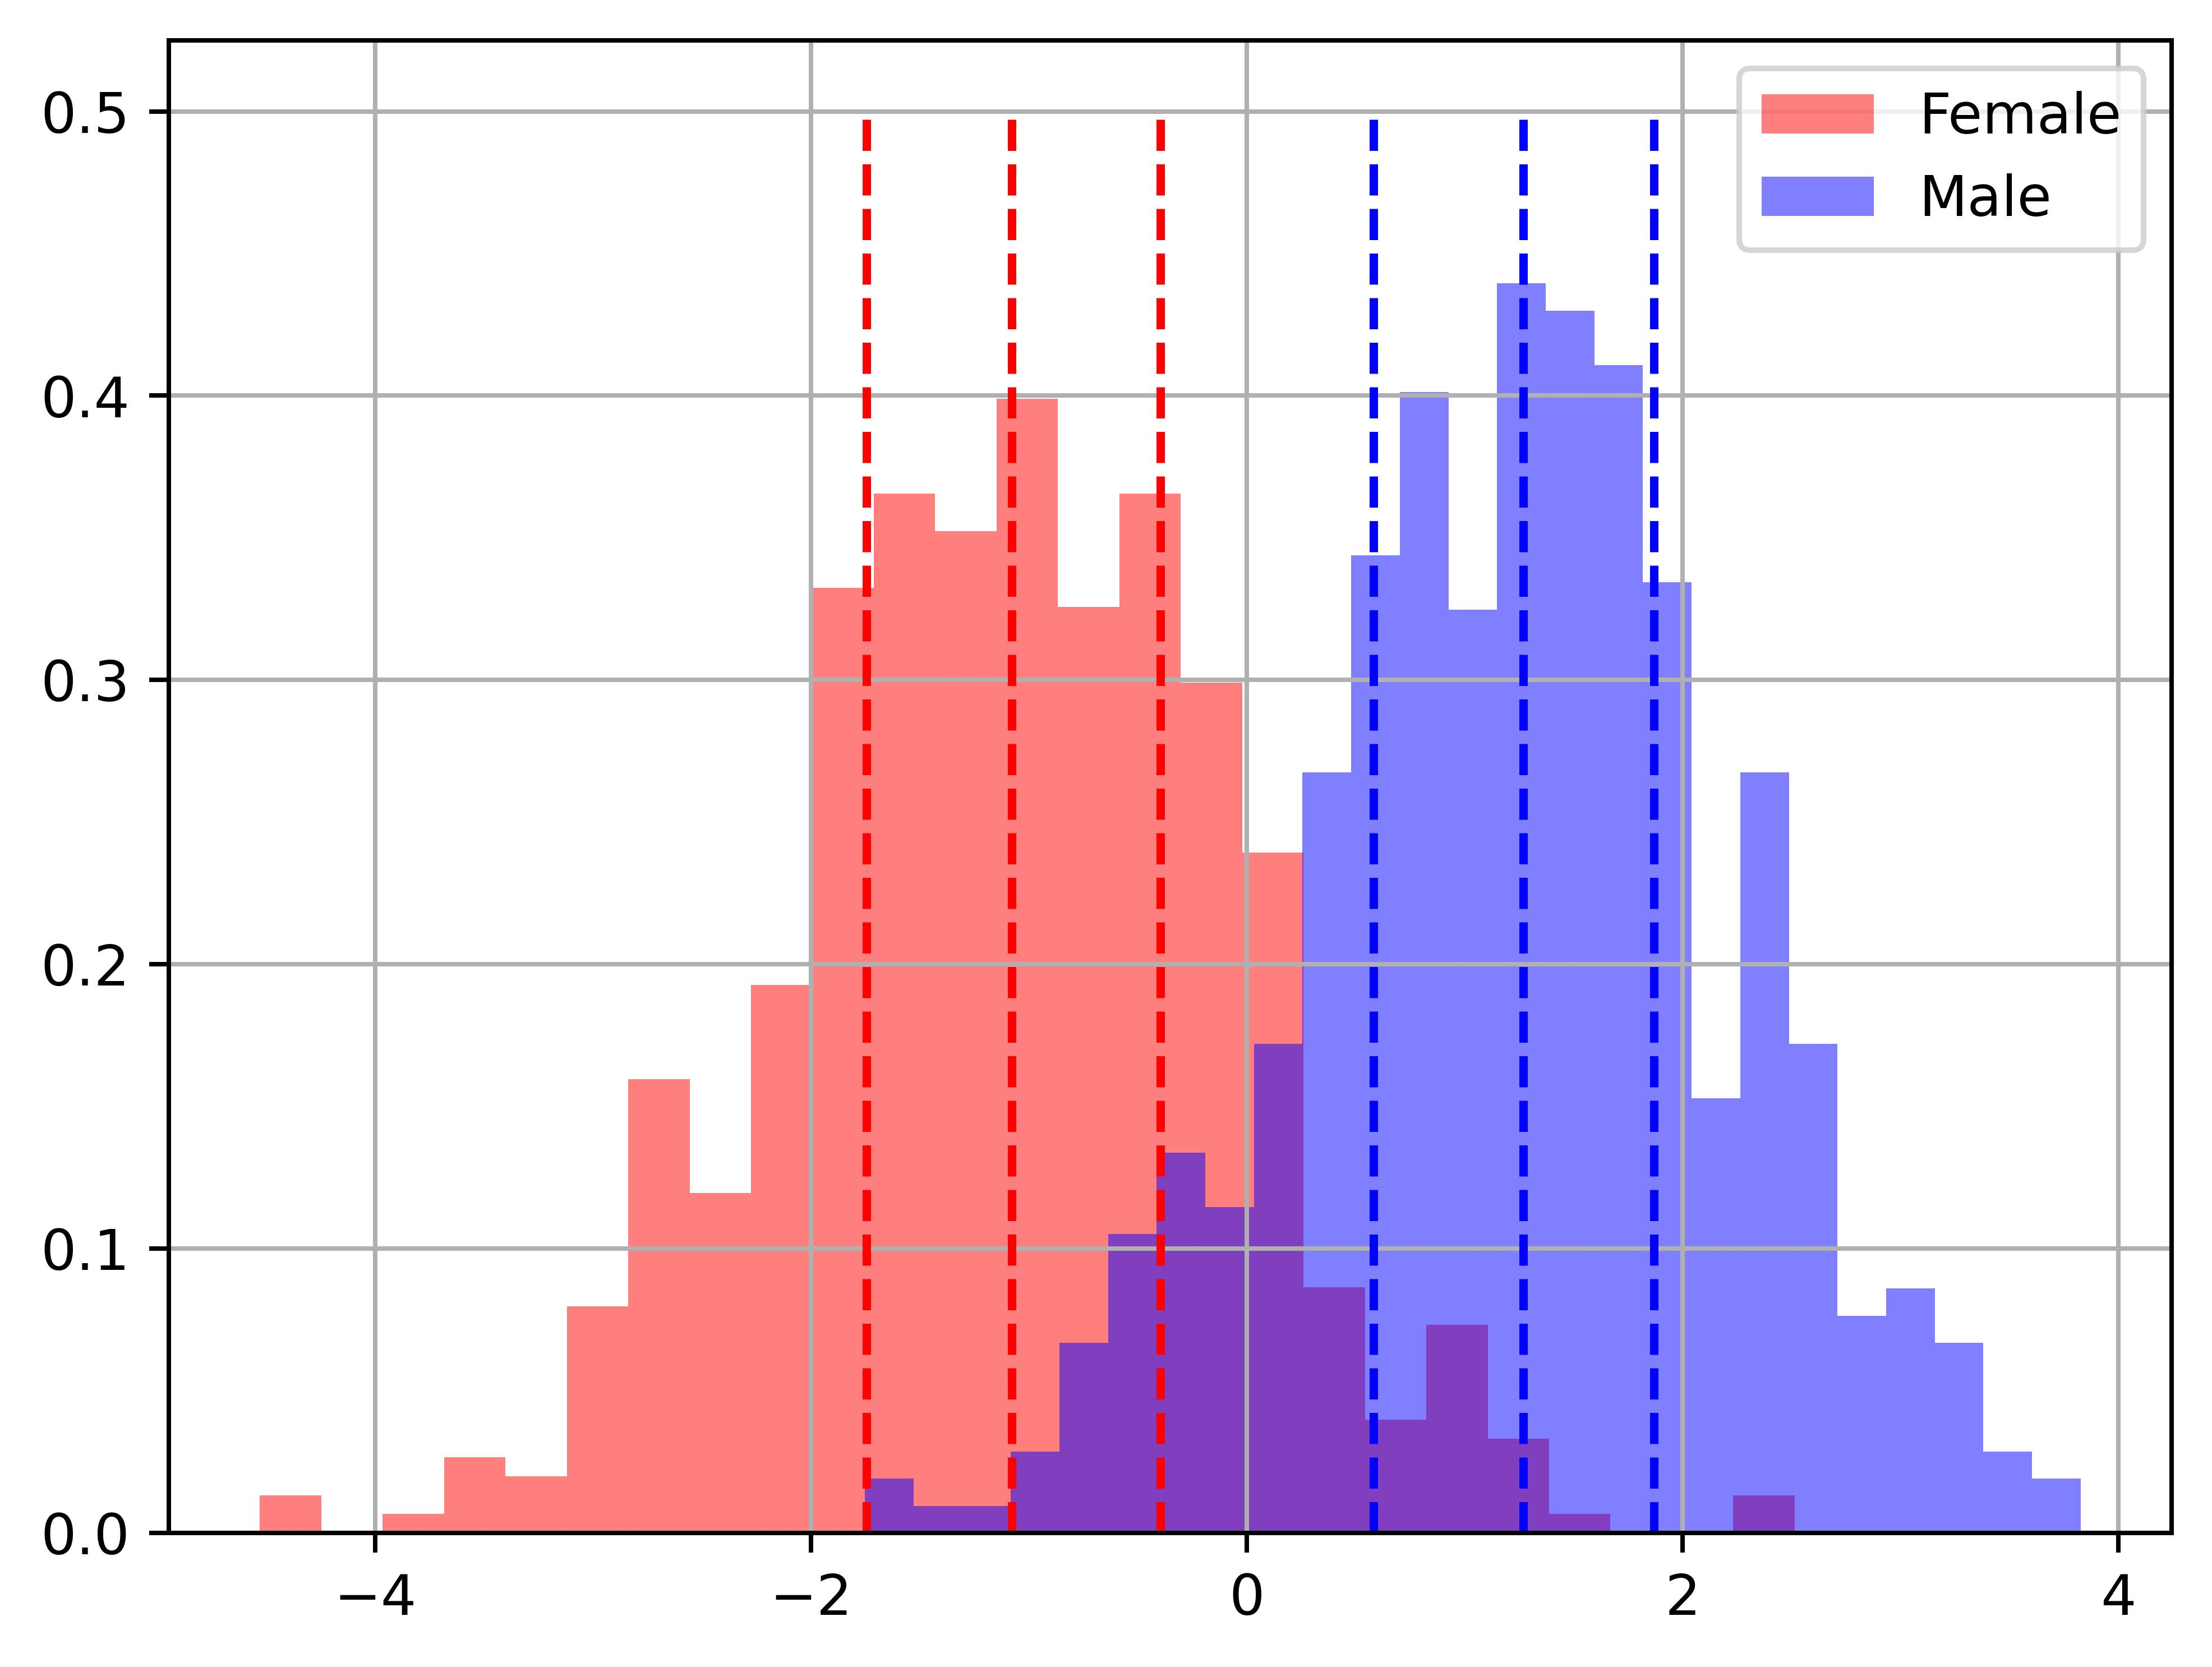
\includegraphics[width=0.4\textwidth]{../Analysis/LDA/node=25_size=480_step=180_rho=0.1/hist_1.jpg}}
    \subfloat[]{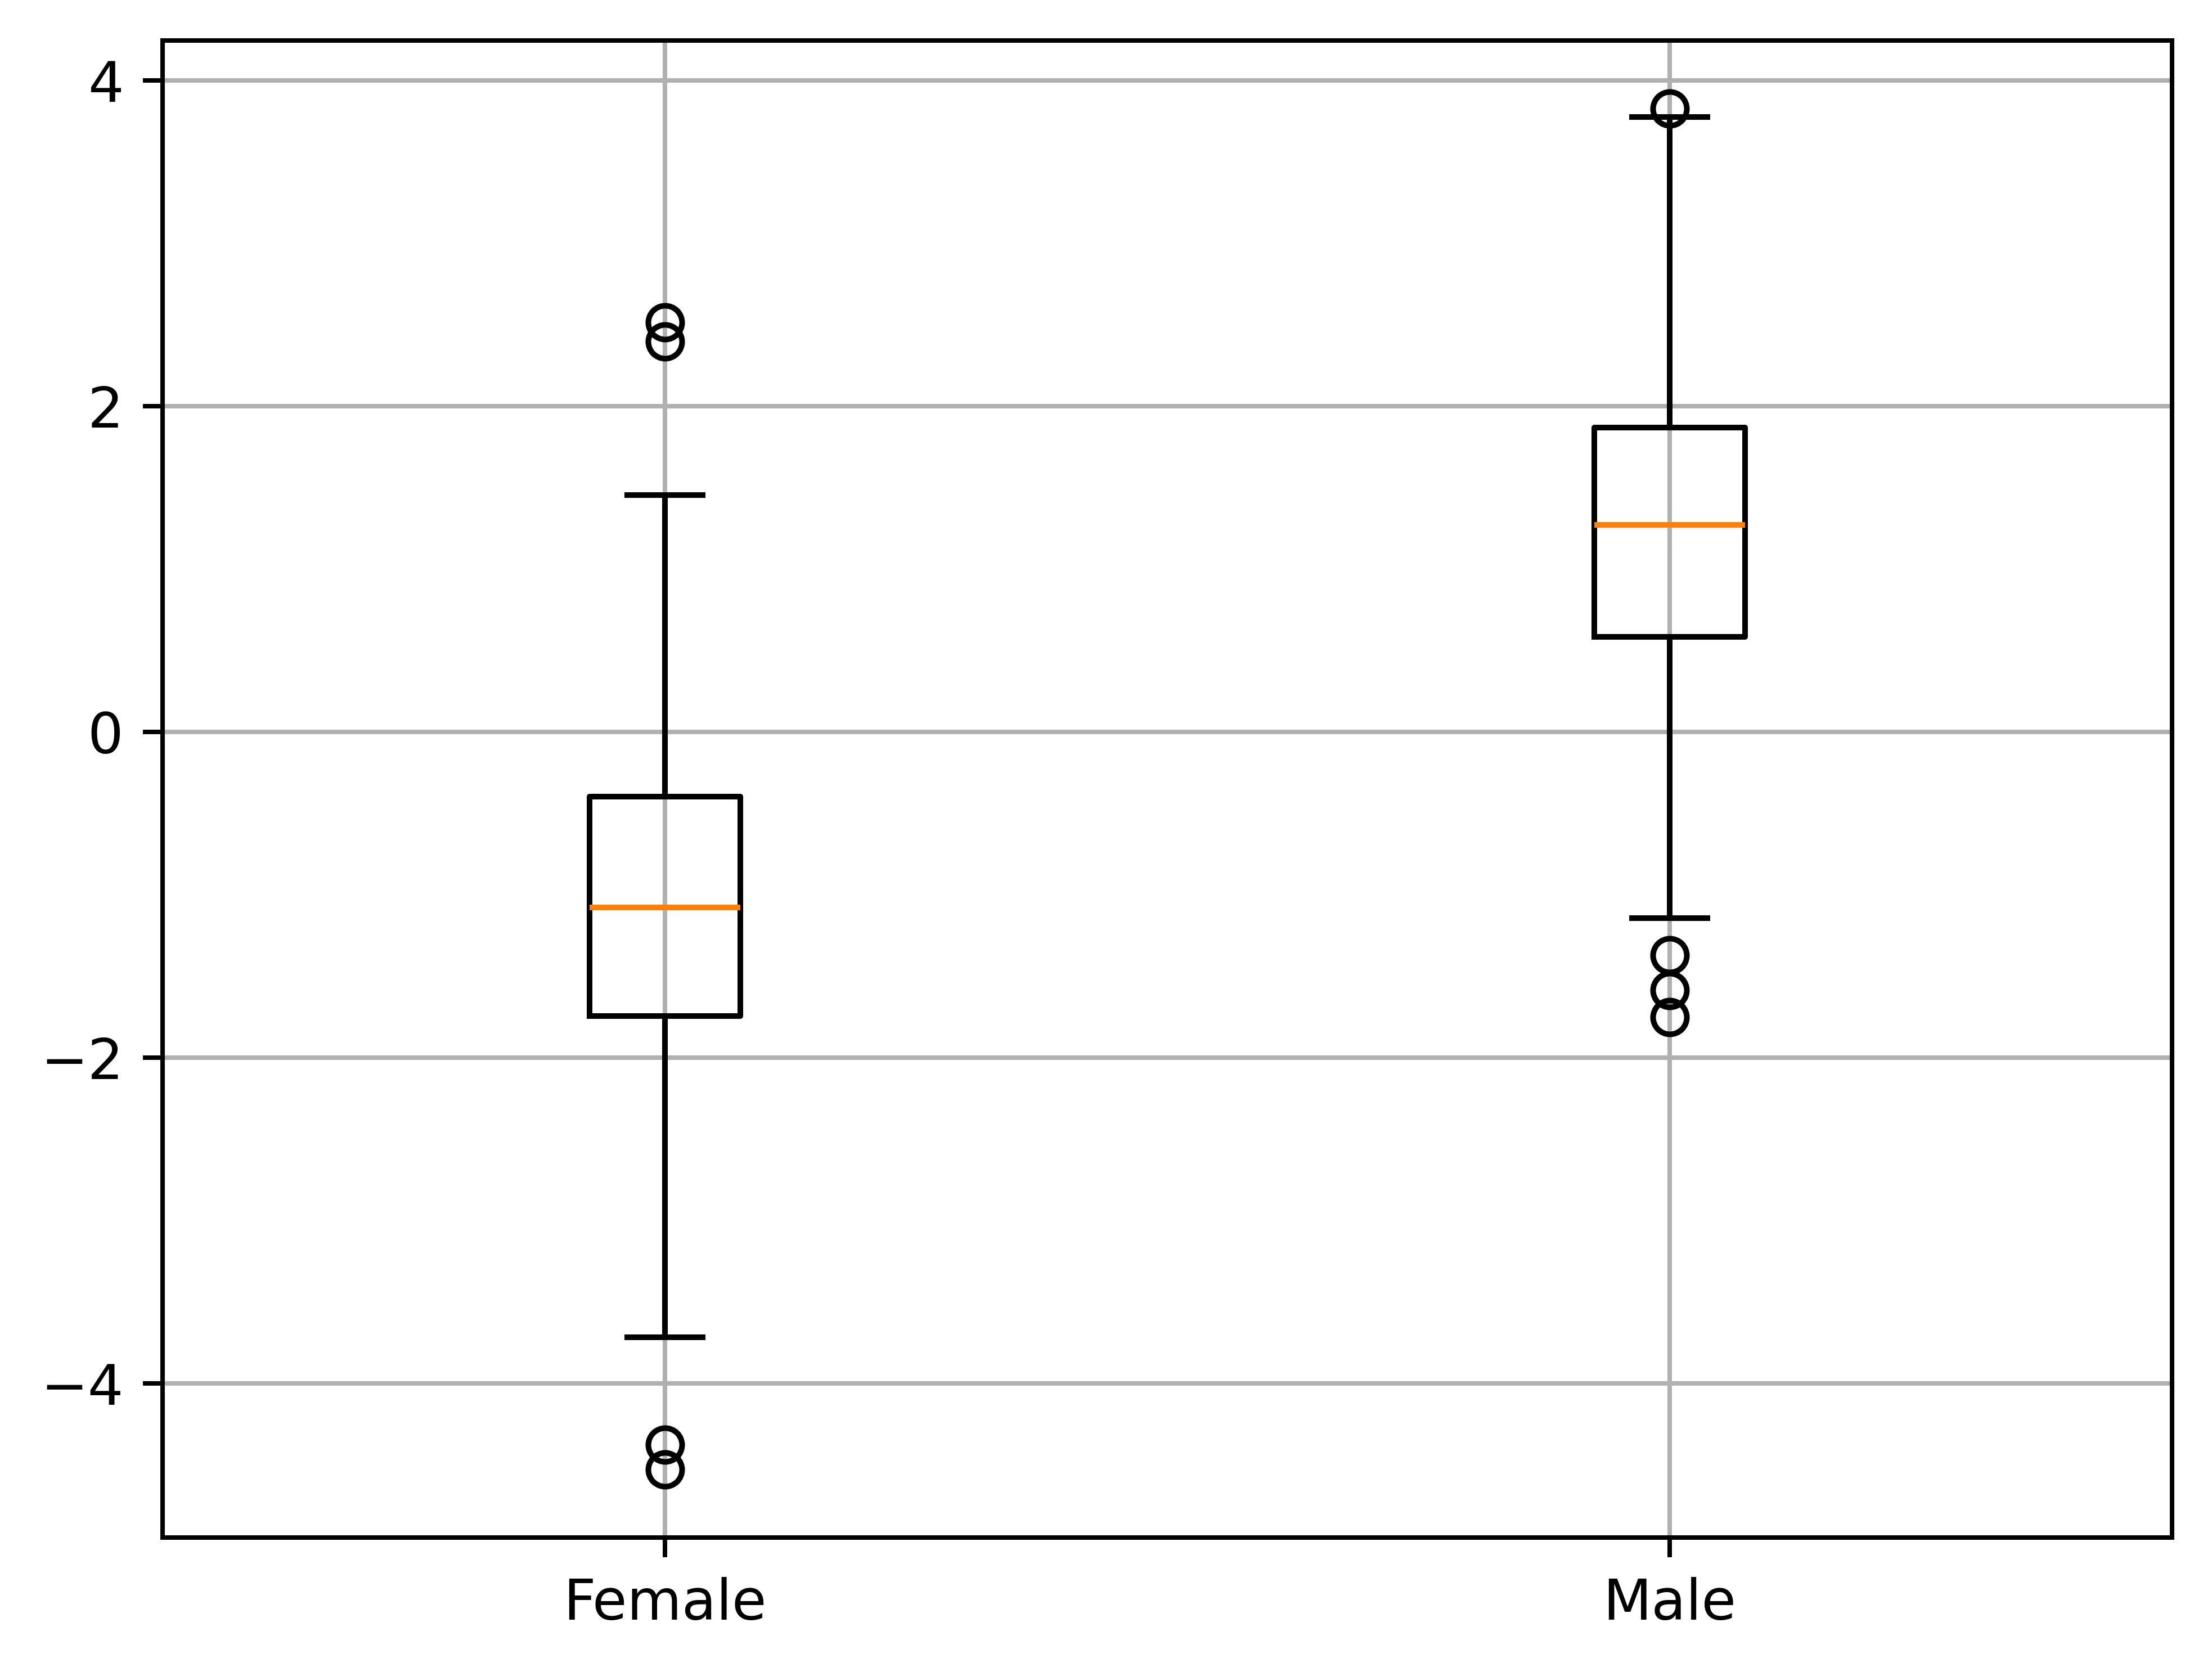
\includegraphics[width=0.4\textwidth]{../Analysis/LDA/node=25_size=480_step=180_rho=0.1/box_1.jpg}} \\
    \subfloat[]{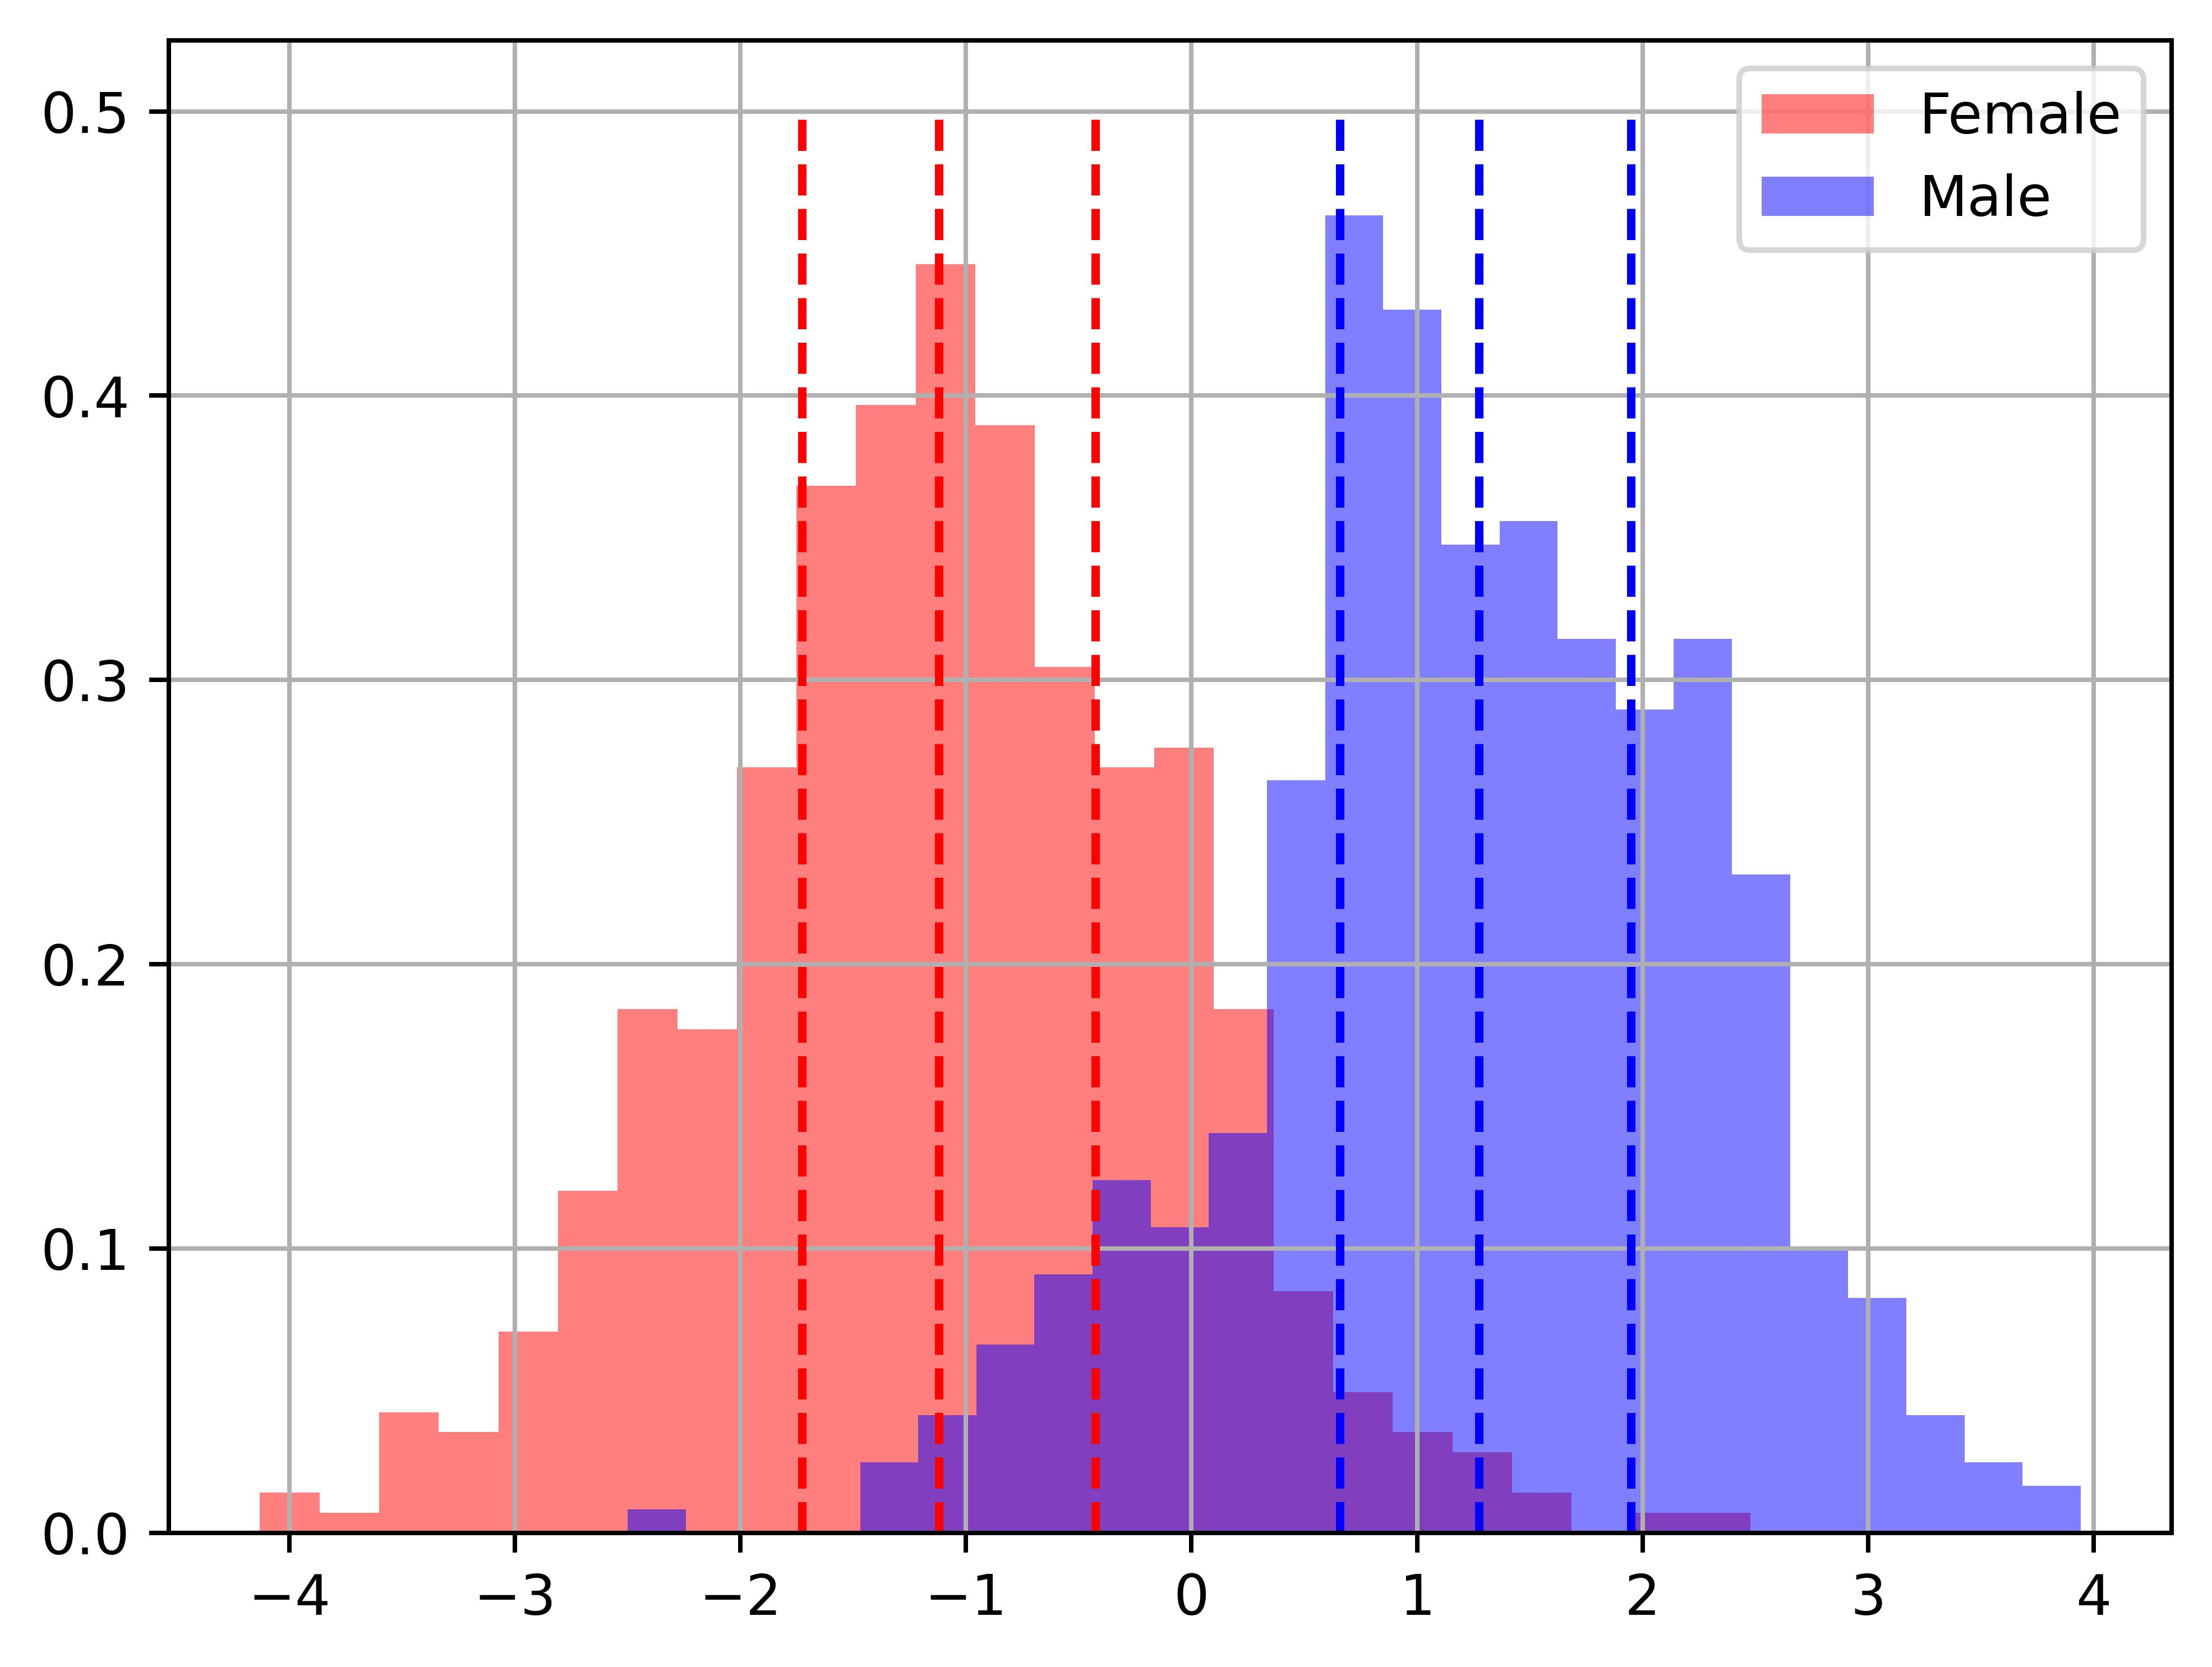
\includegraphics[width=0.4\textwidth]{../Analysis/LDA/node=25_size=480_step=180_rho=0.1/hist_2.jpg}}
    \subfloat[]{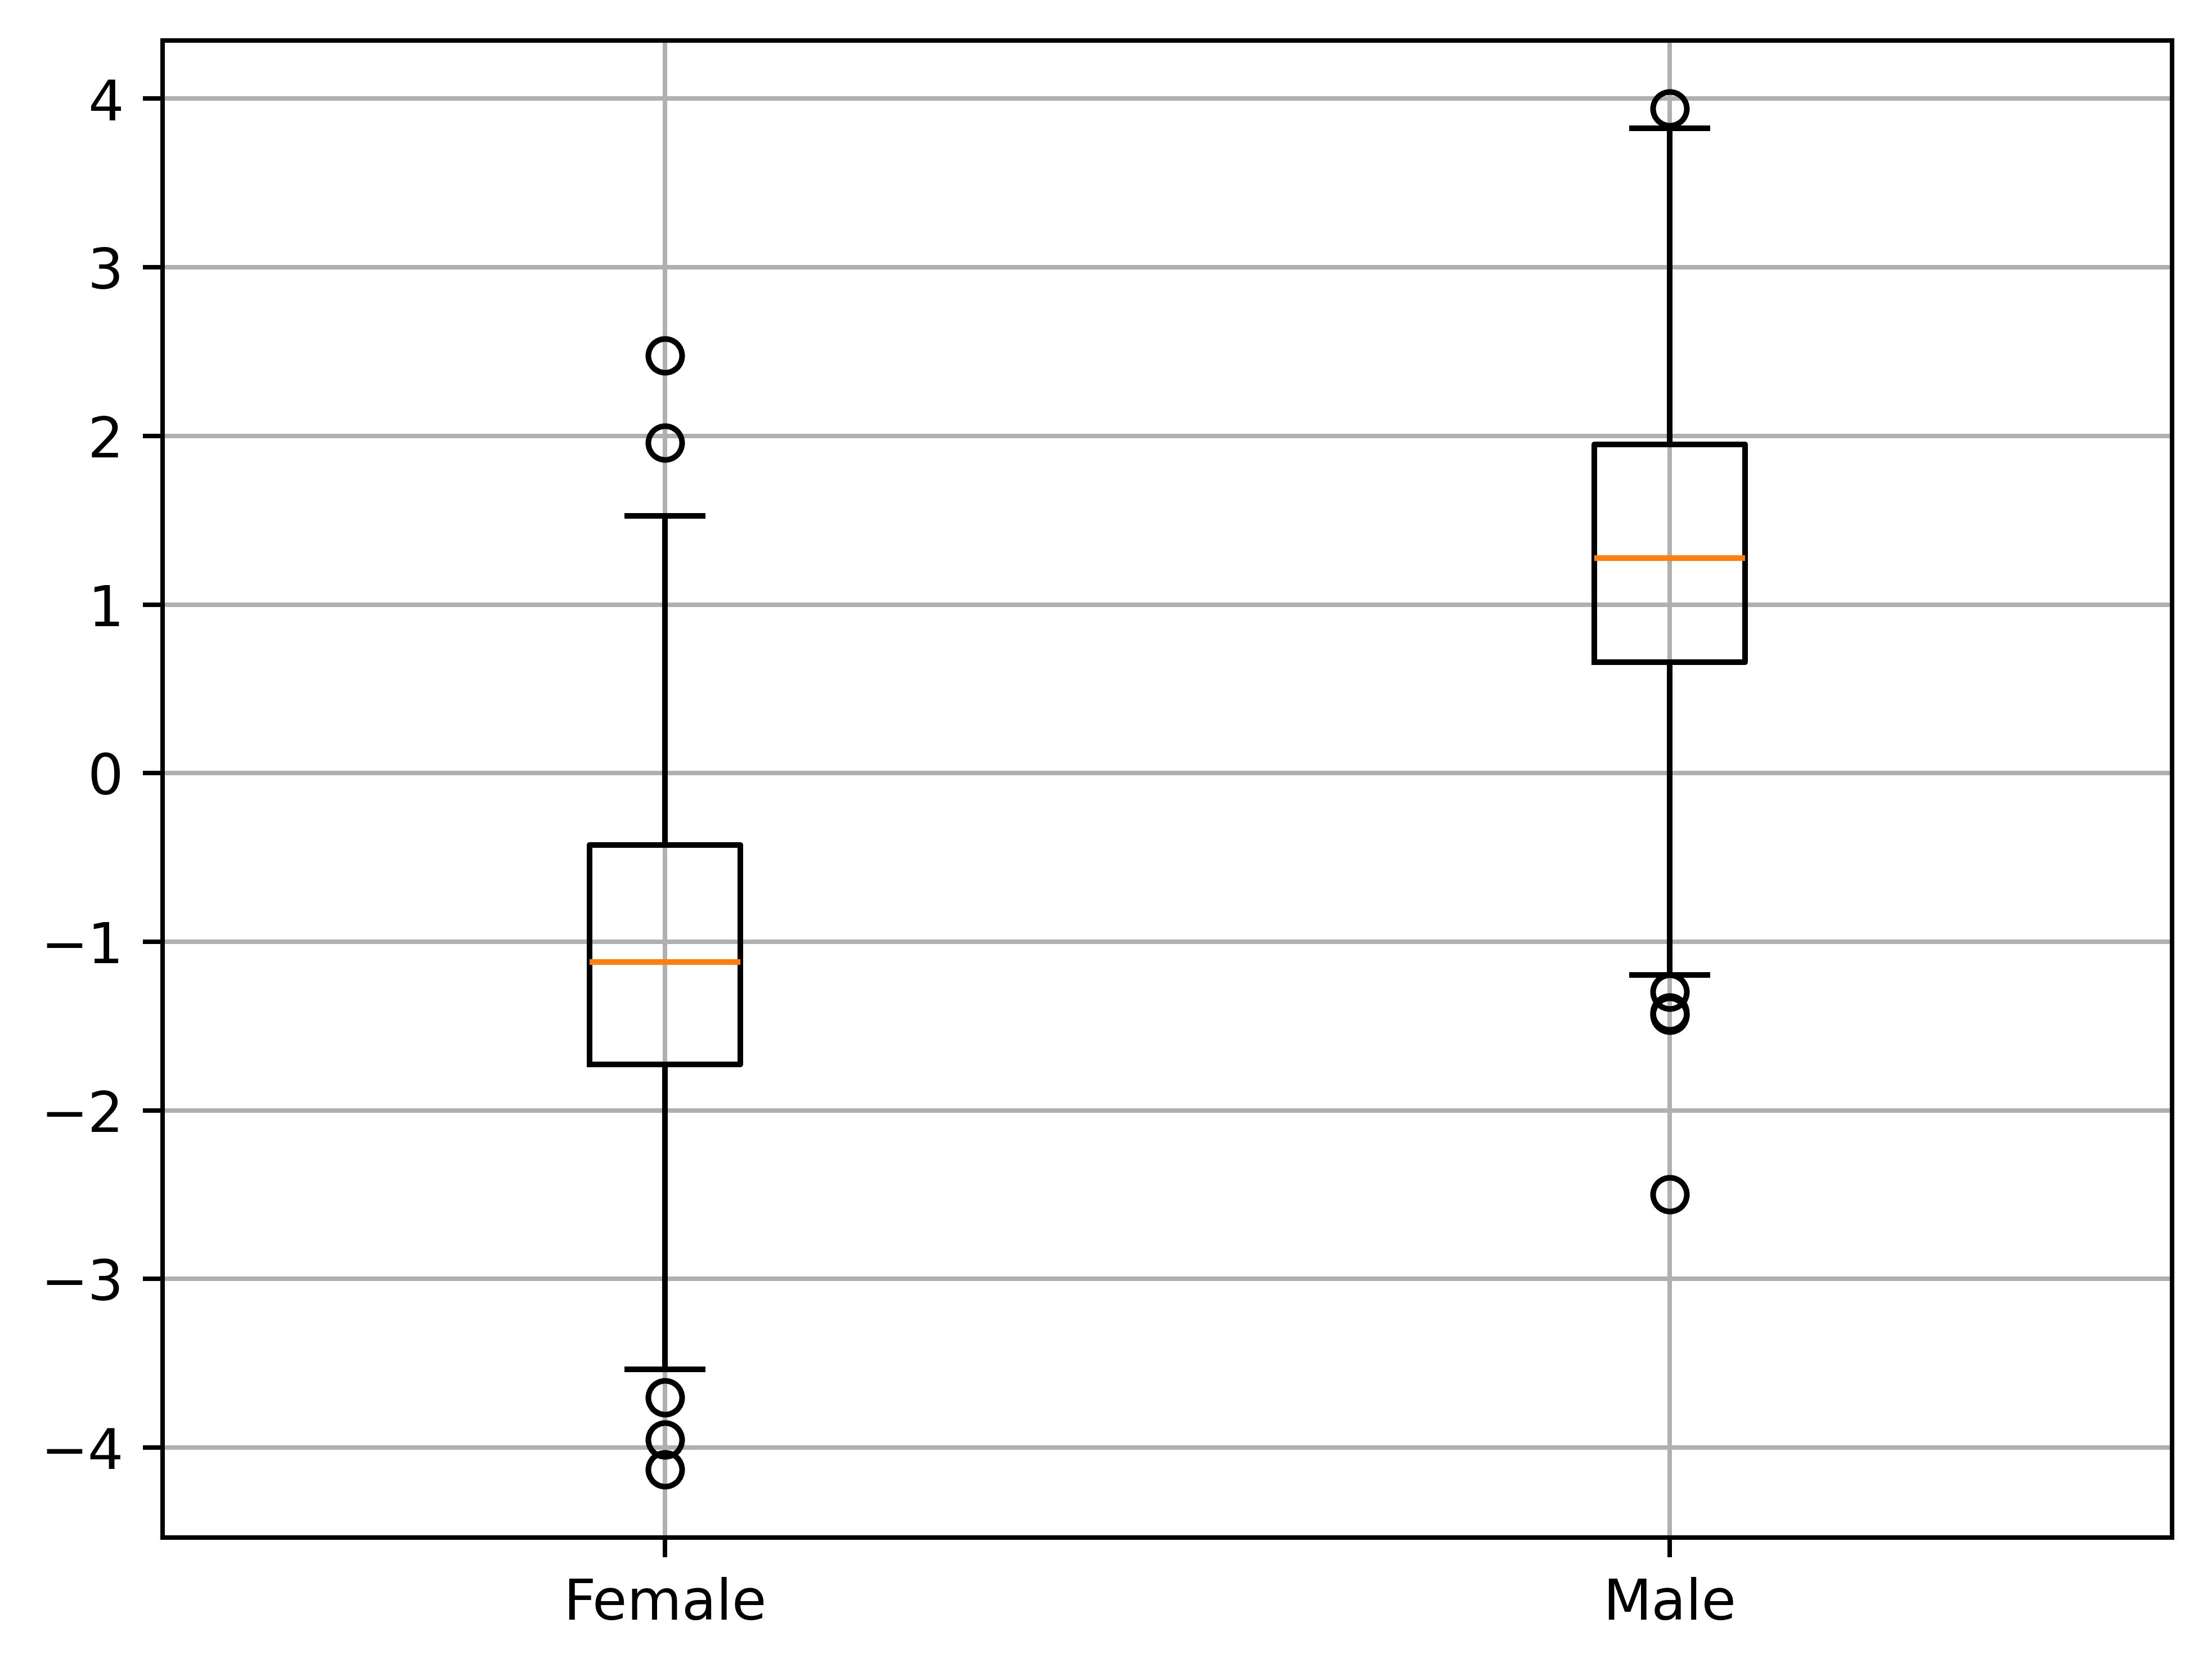
\includegraphics[width=0.4\textwidth]{../Analysis/LDA/node=25_size=480_step=180_rho=0.1/box_2.jpg}} \\
    \caption{LDA for Dynamic connectivity with $N_{node} = 25$.}
    \label{LDA-example-4}
\end{figure}

\begin{figure}[H]
    \centering
    \subfloat[]{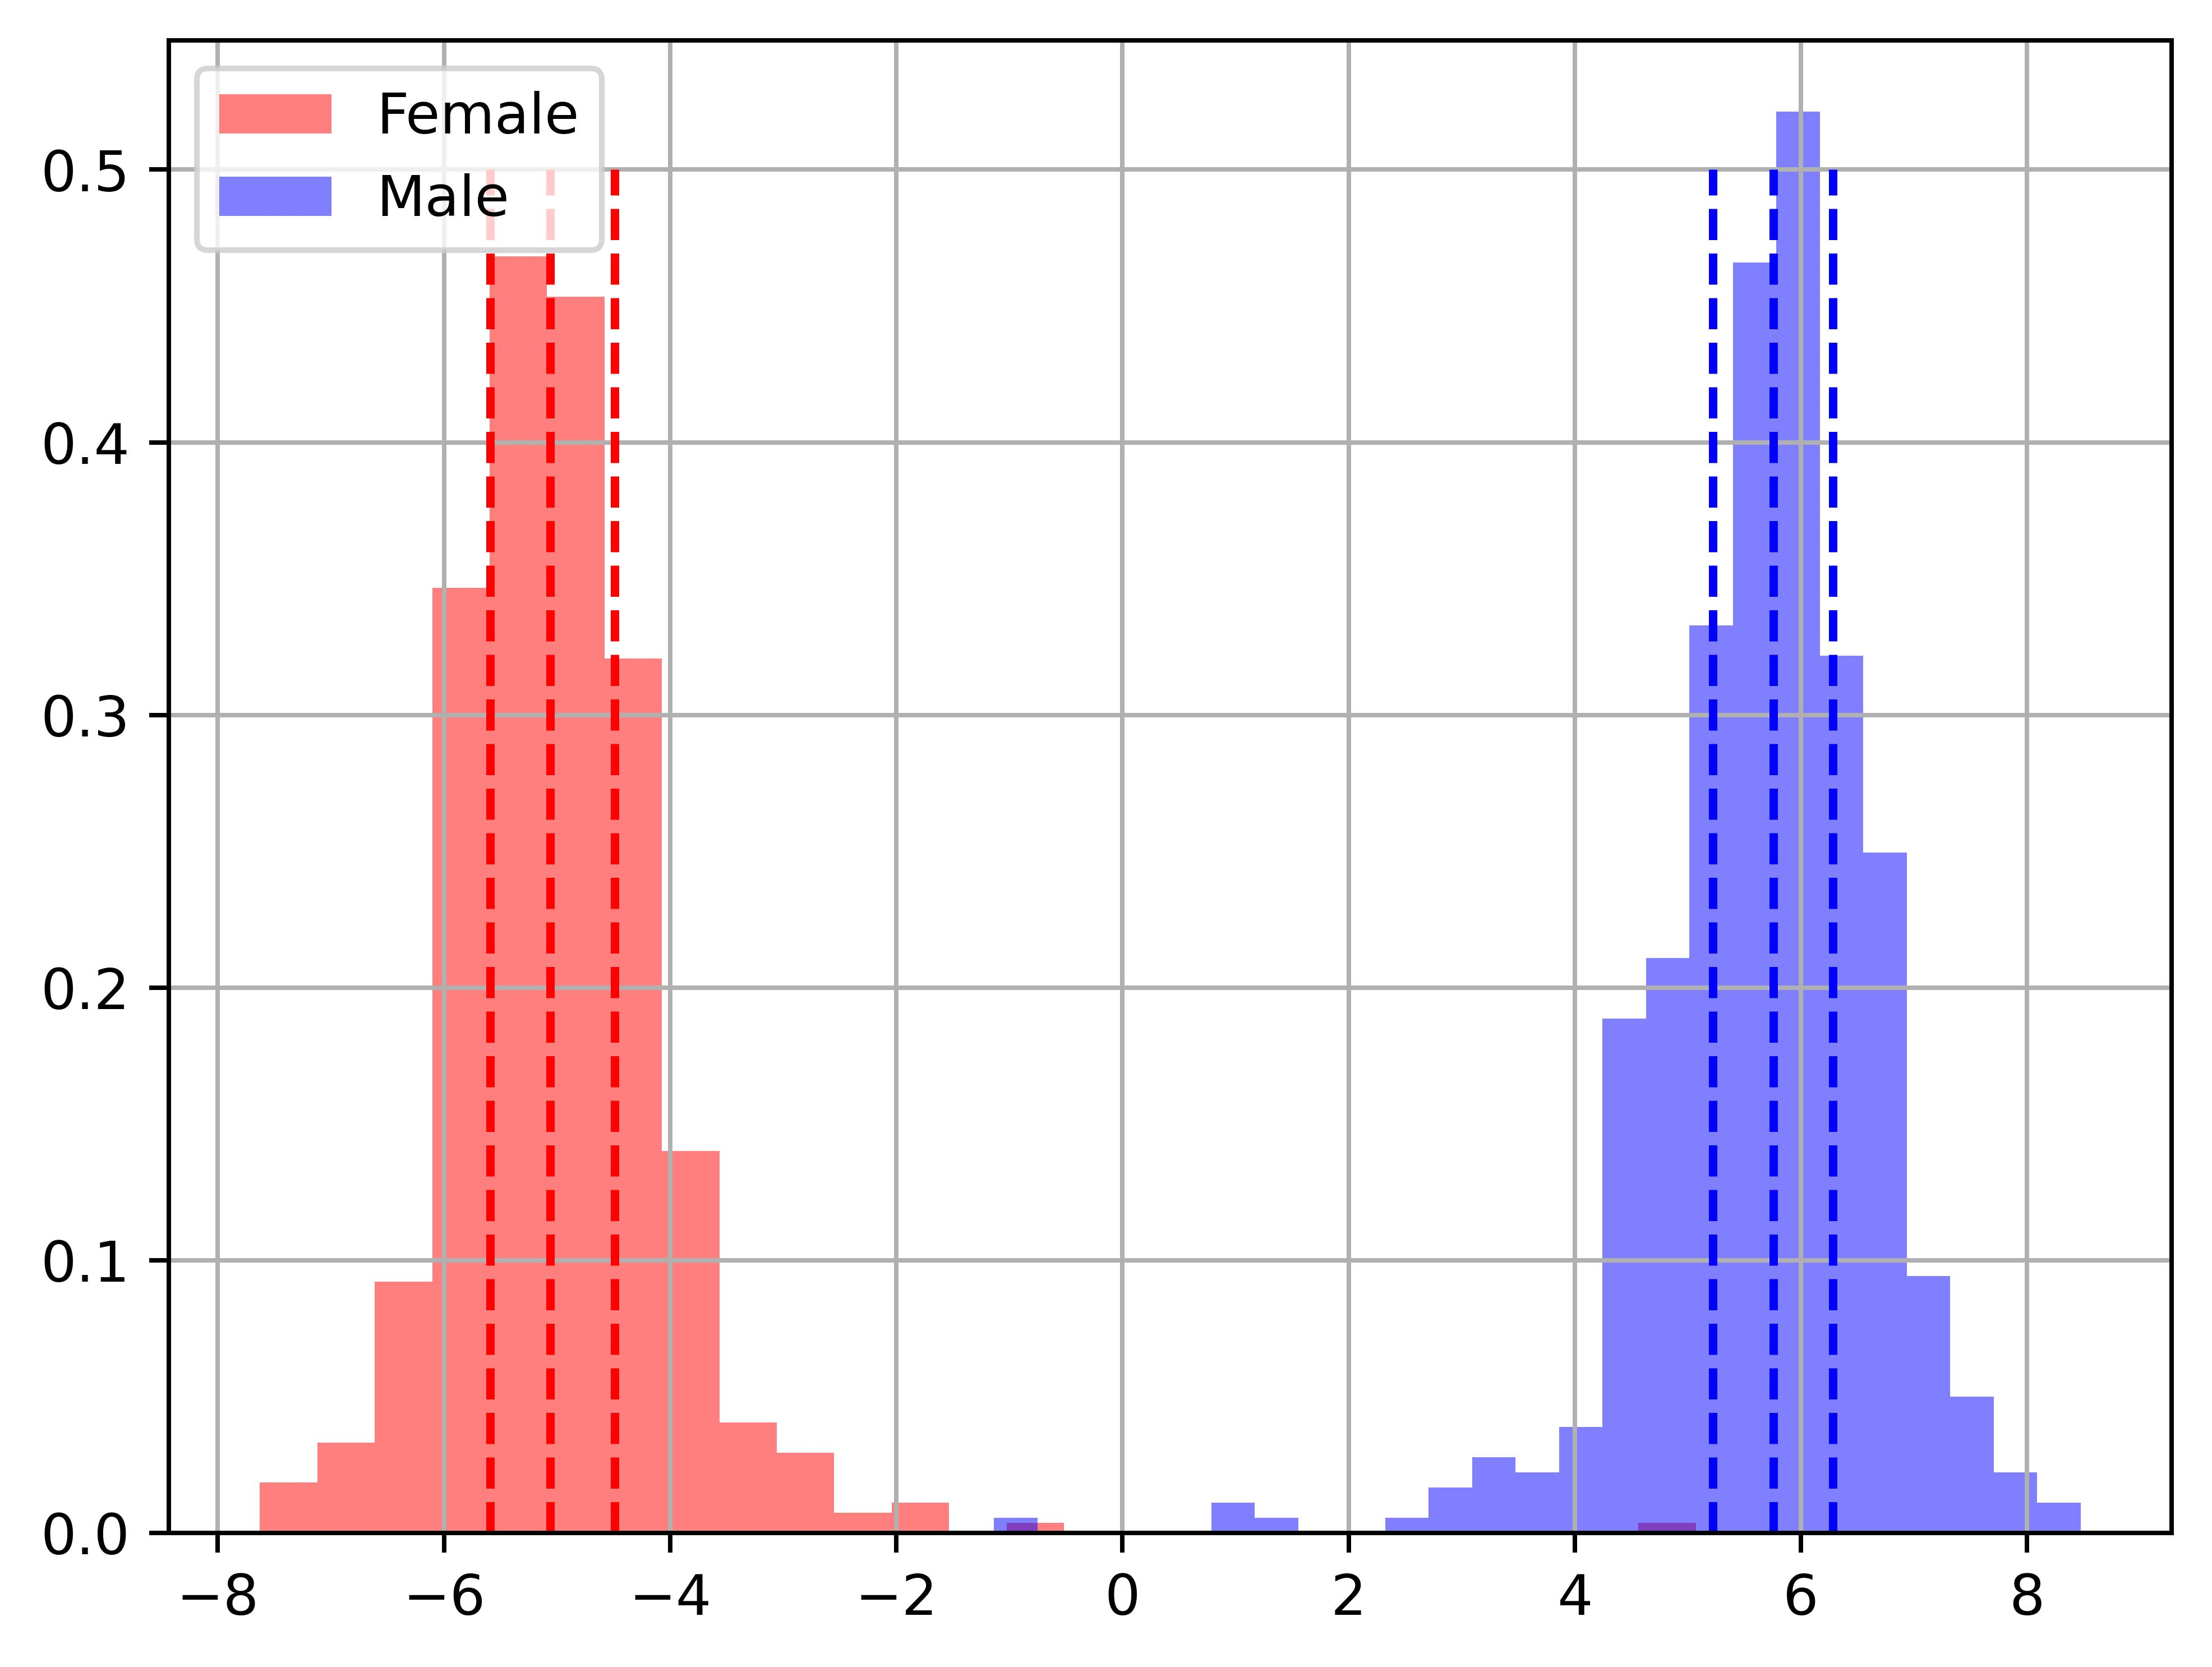
\includegraphics[width=0.4\textwidth]{../Analysis/LDA/node=50_size=4800_step=4800_rho=0.1/hist_0.jpg}}
    \subfloat[]{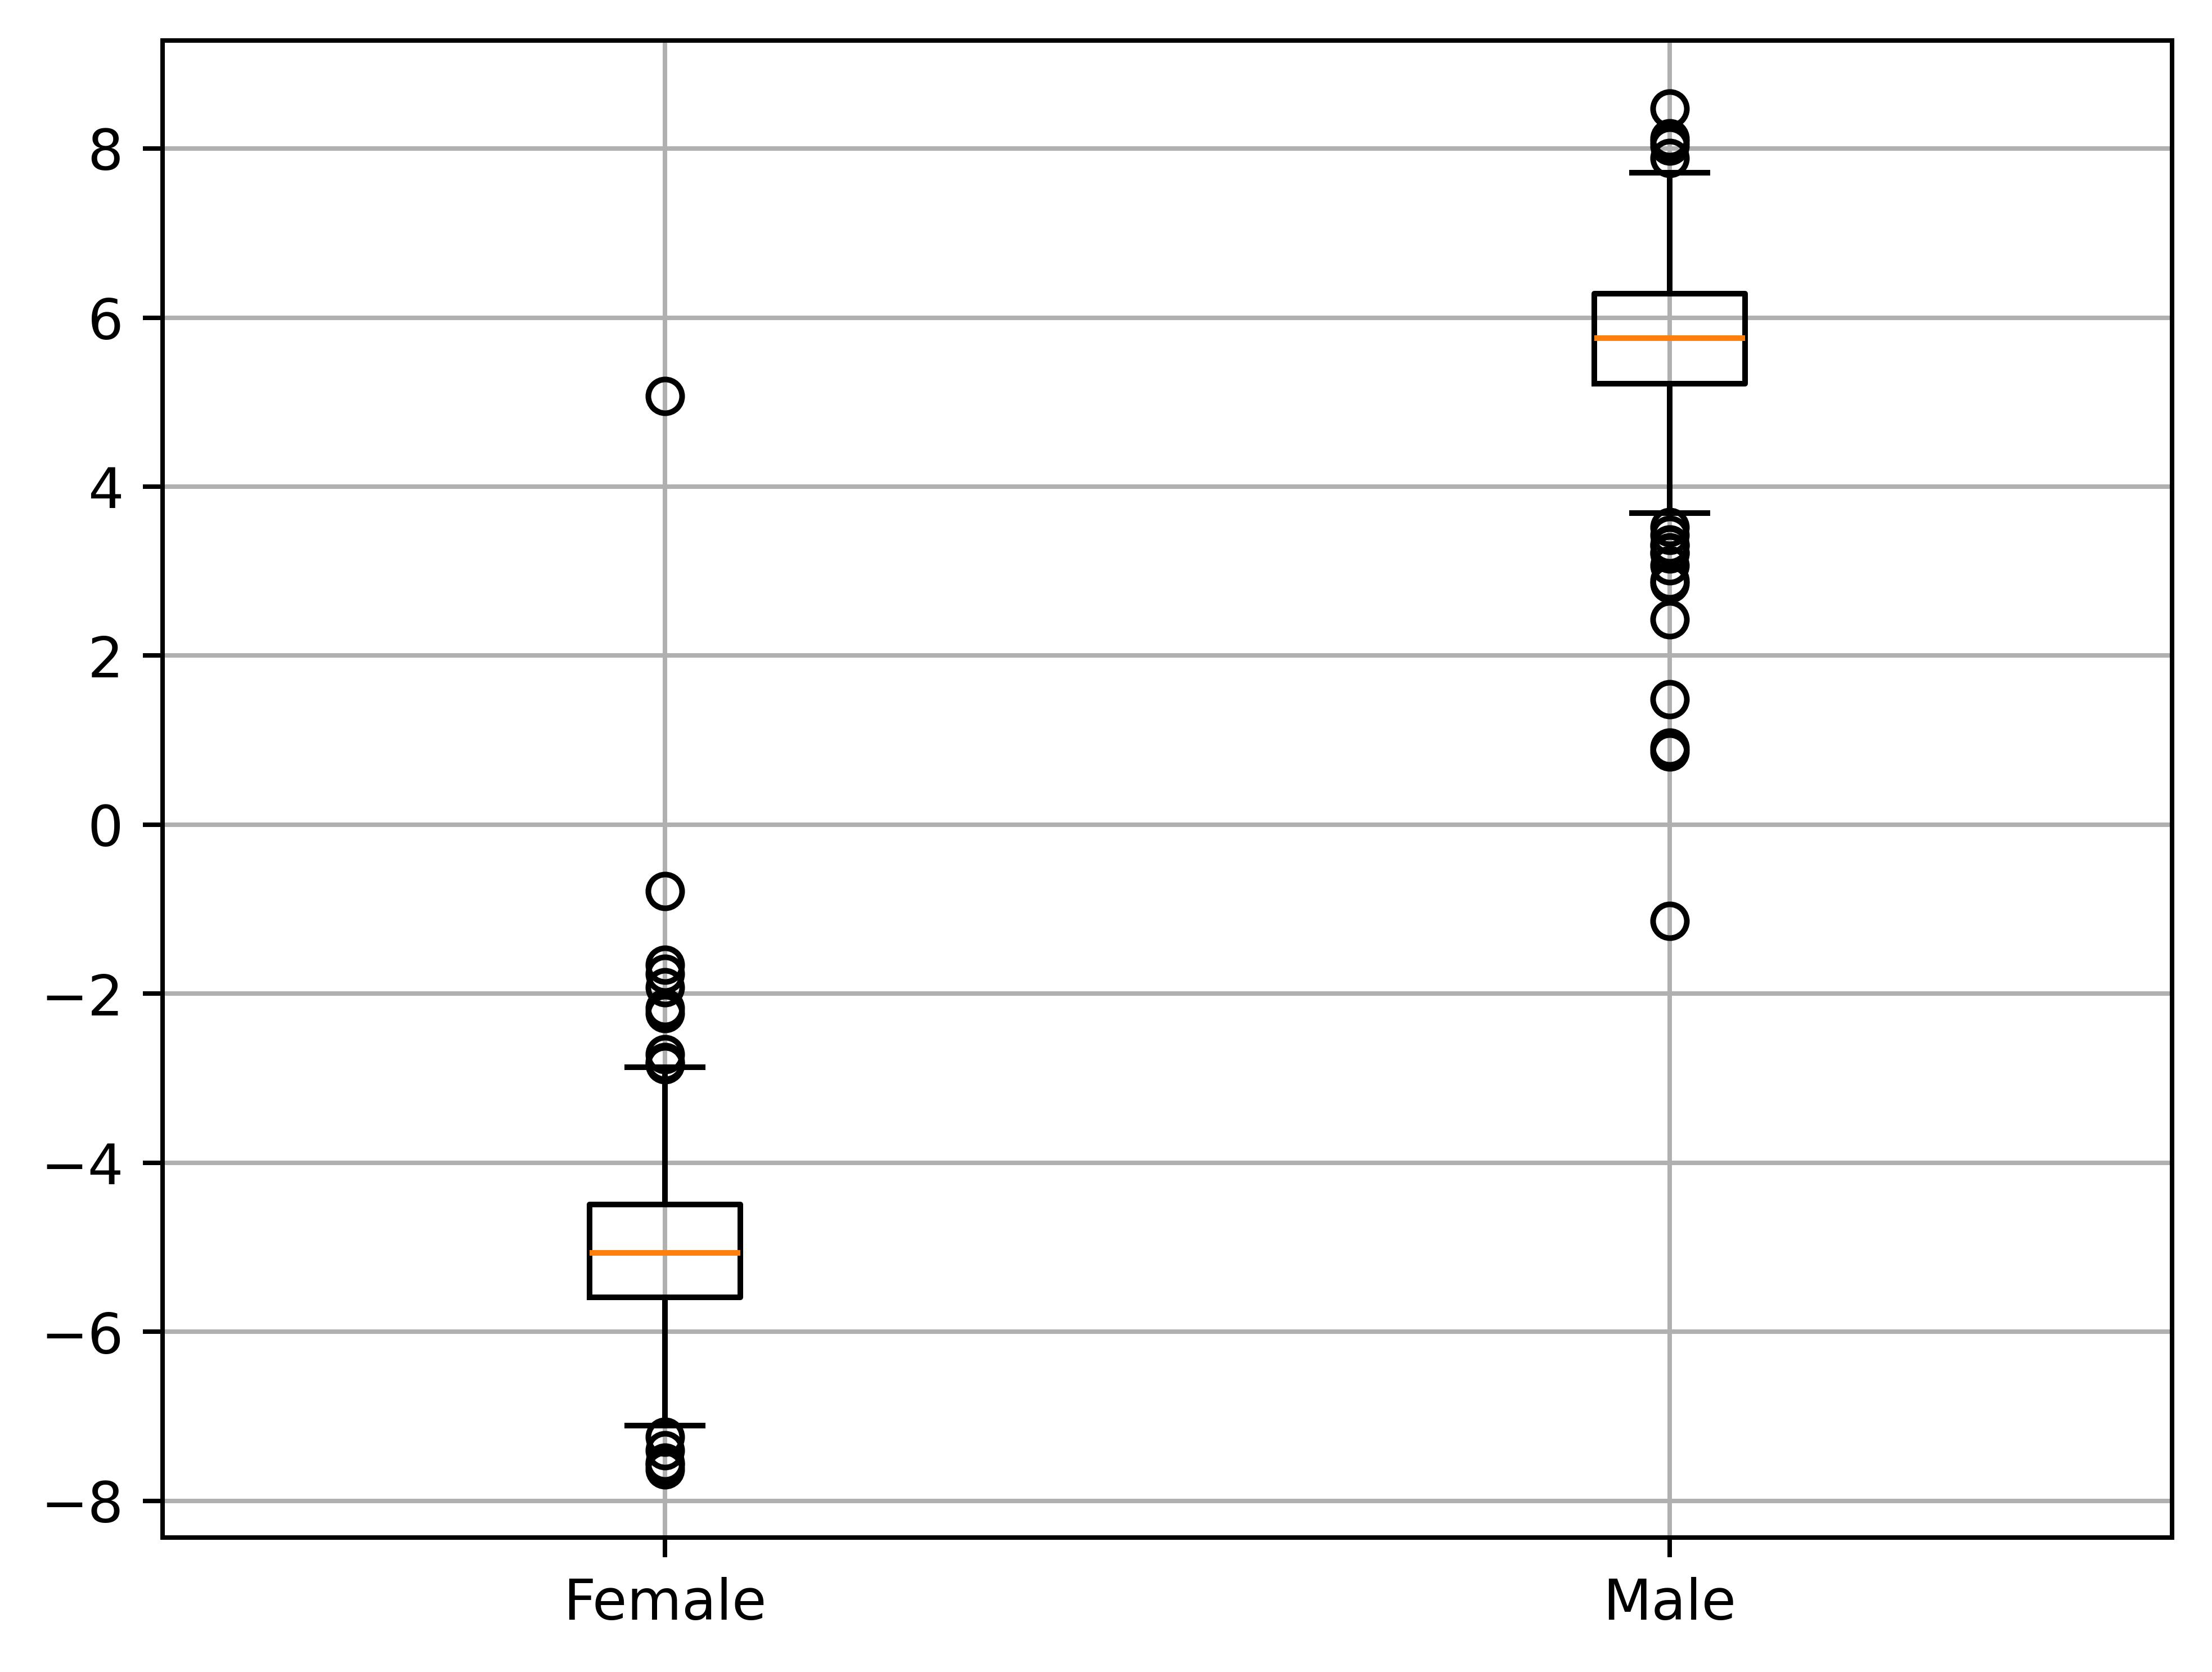
\includegraphics[width=0.4\textwidth]{../Analysis/LDA/node=50_size=4800_step=4800_rho=0.1/box_0.jpg}} \\
    \caption{LDA for static connectivity with $N_{node} = 50$.}
    \label{LDA-example-5}
\end{figure}

\begin{figure}[H]
    \centering
    \subfloat[]{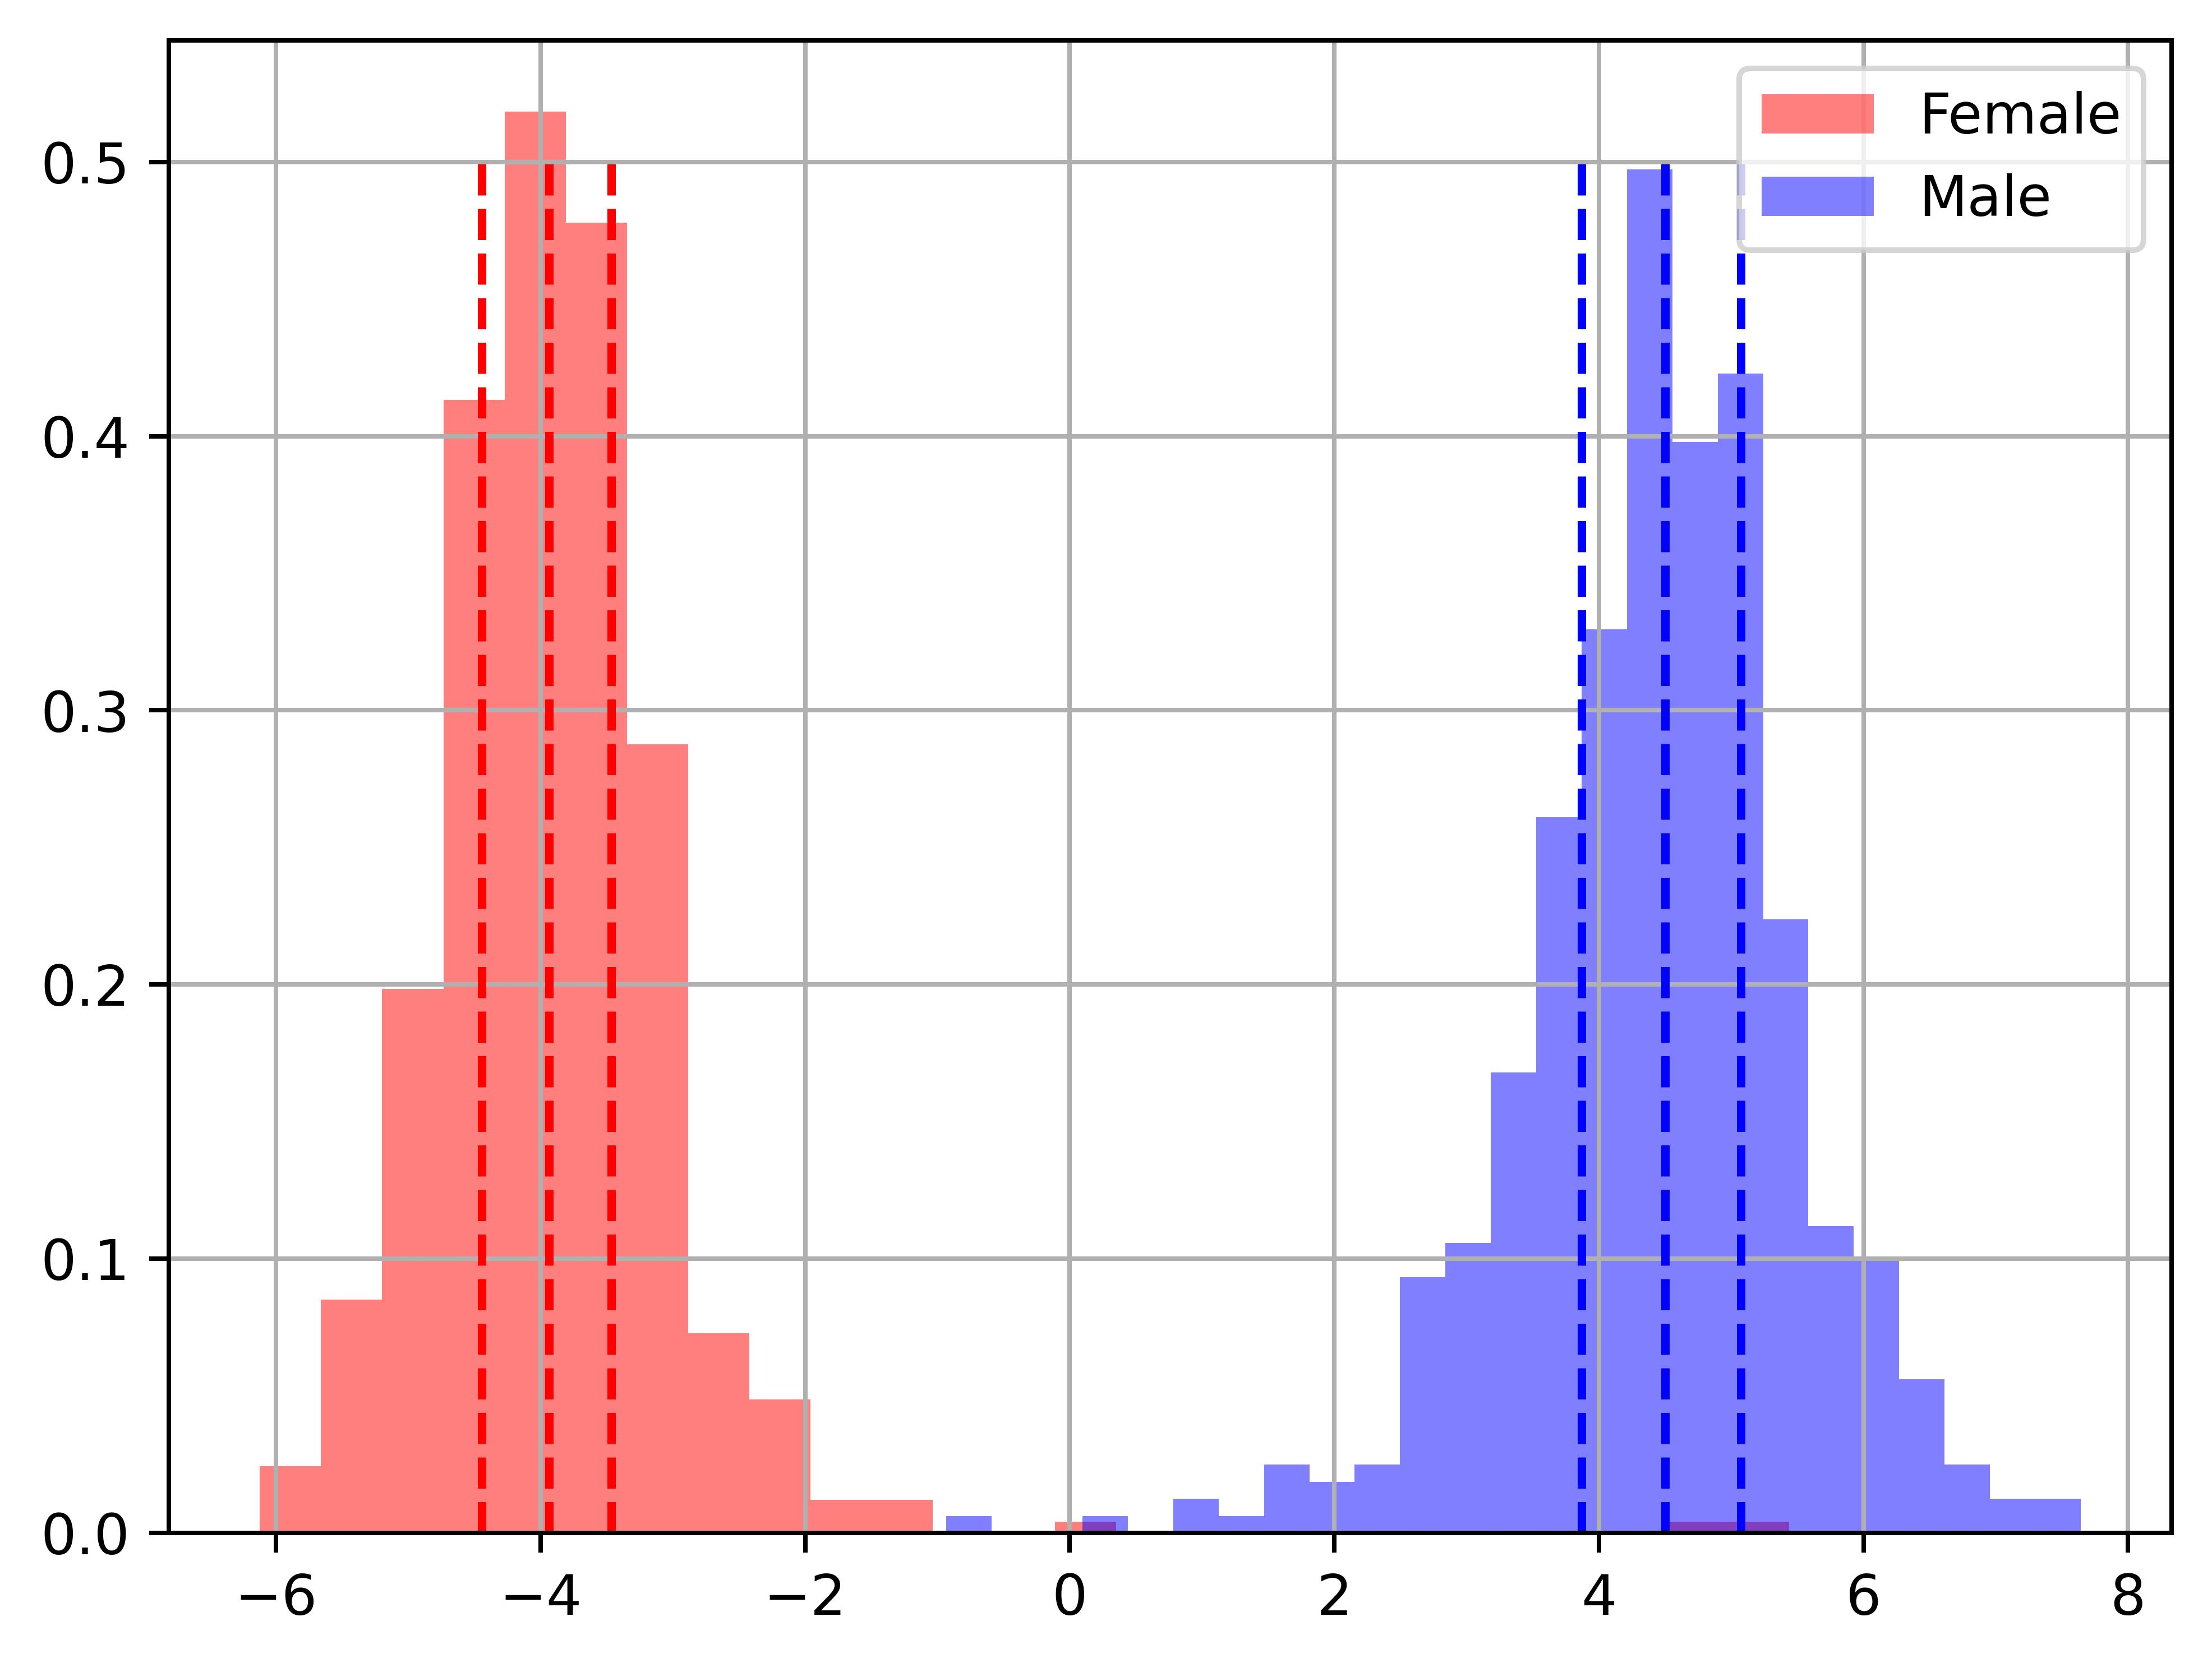
\includegraphics[width=0.4\textwidth]{../Analysis/LDA/node=50_size=480_step=180_rho=0.1/hist_0.jpg}}
    \subfloat[]{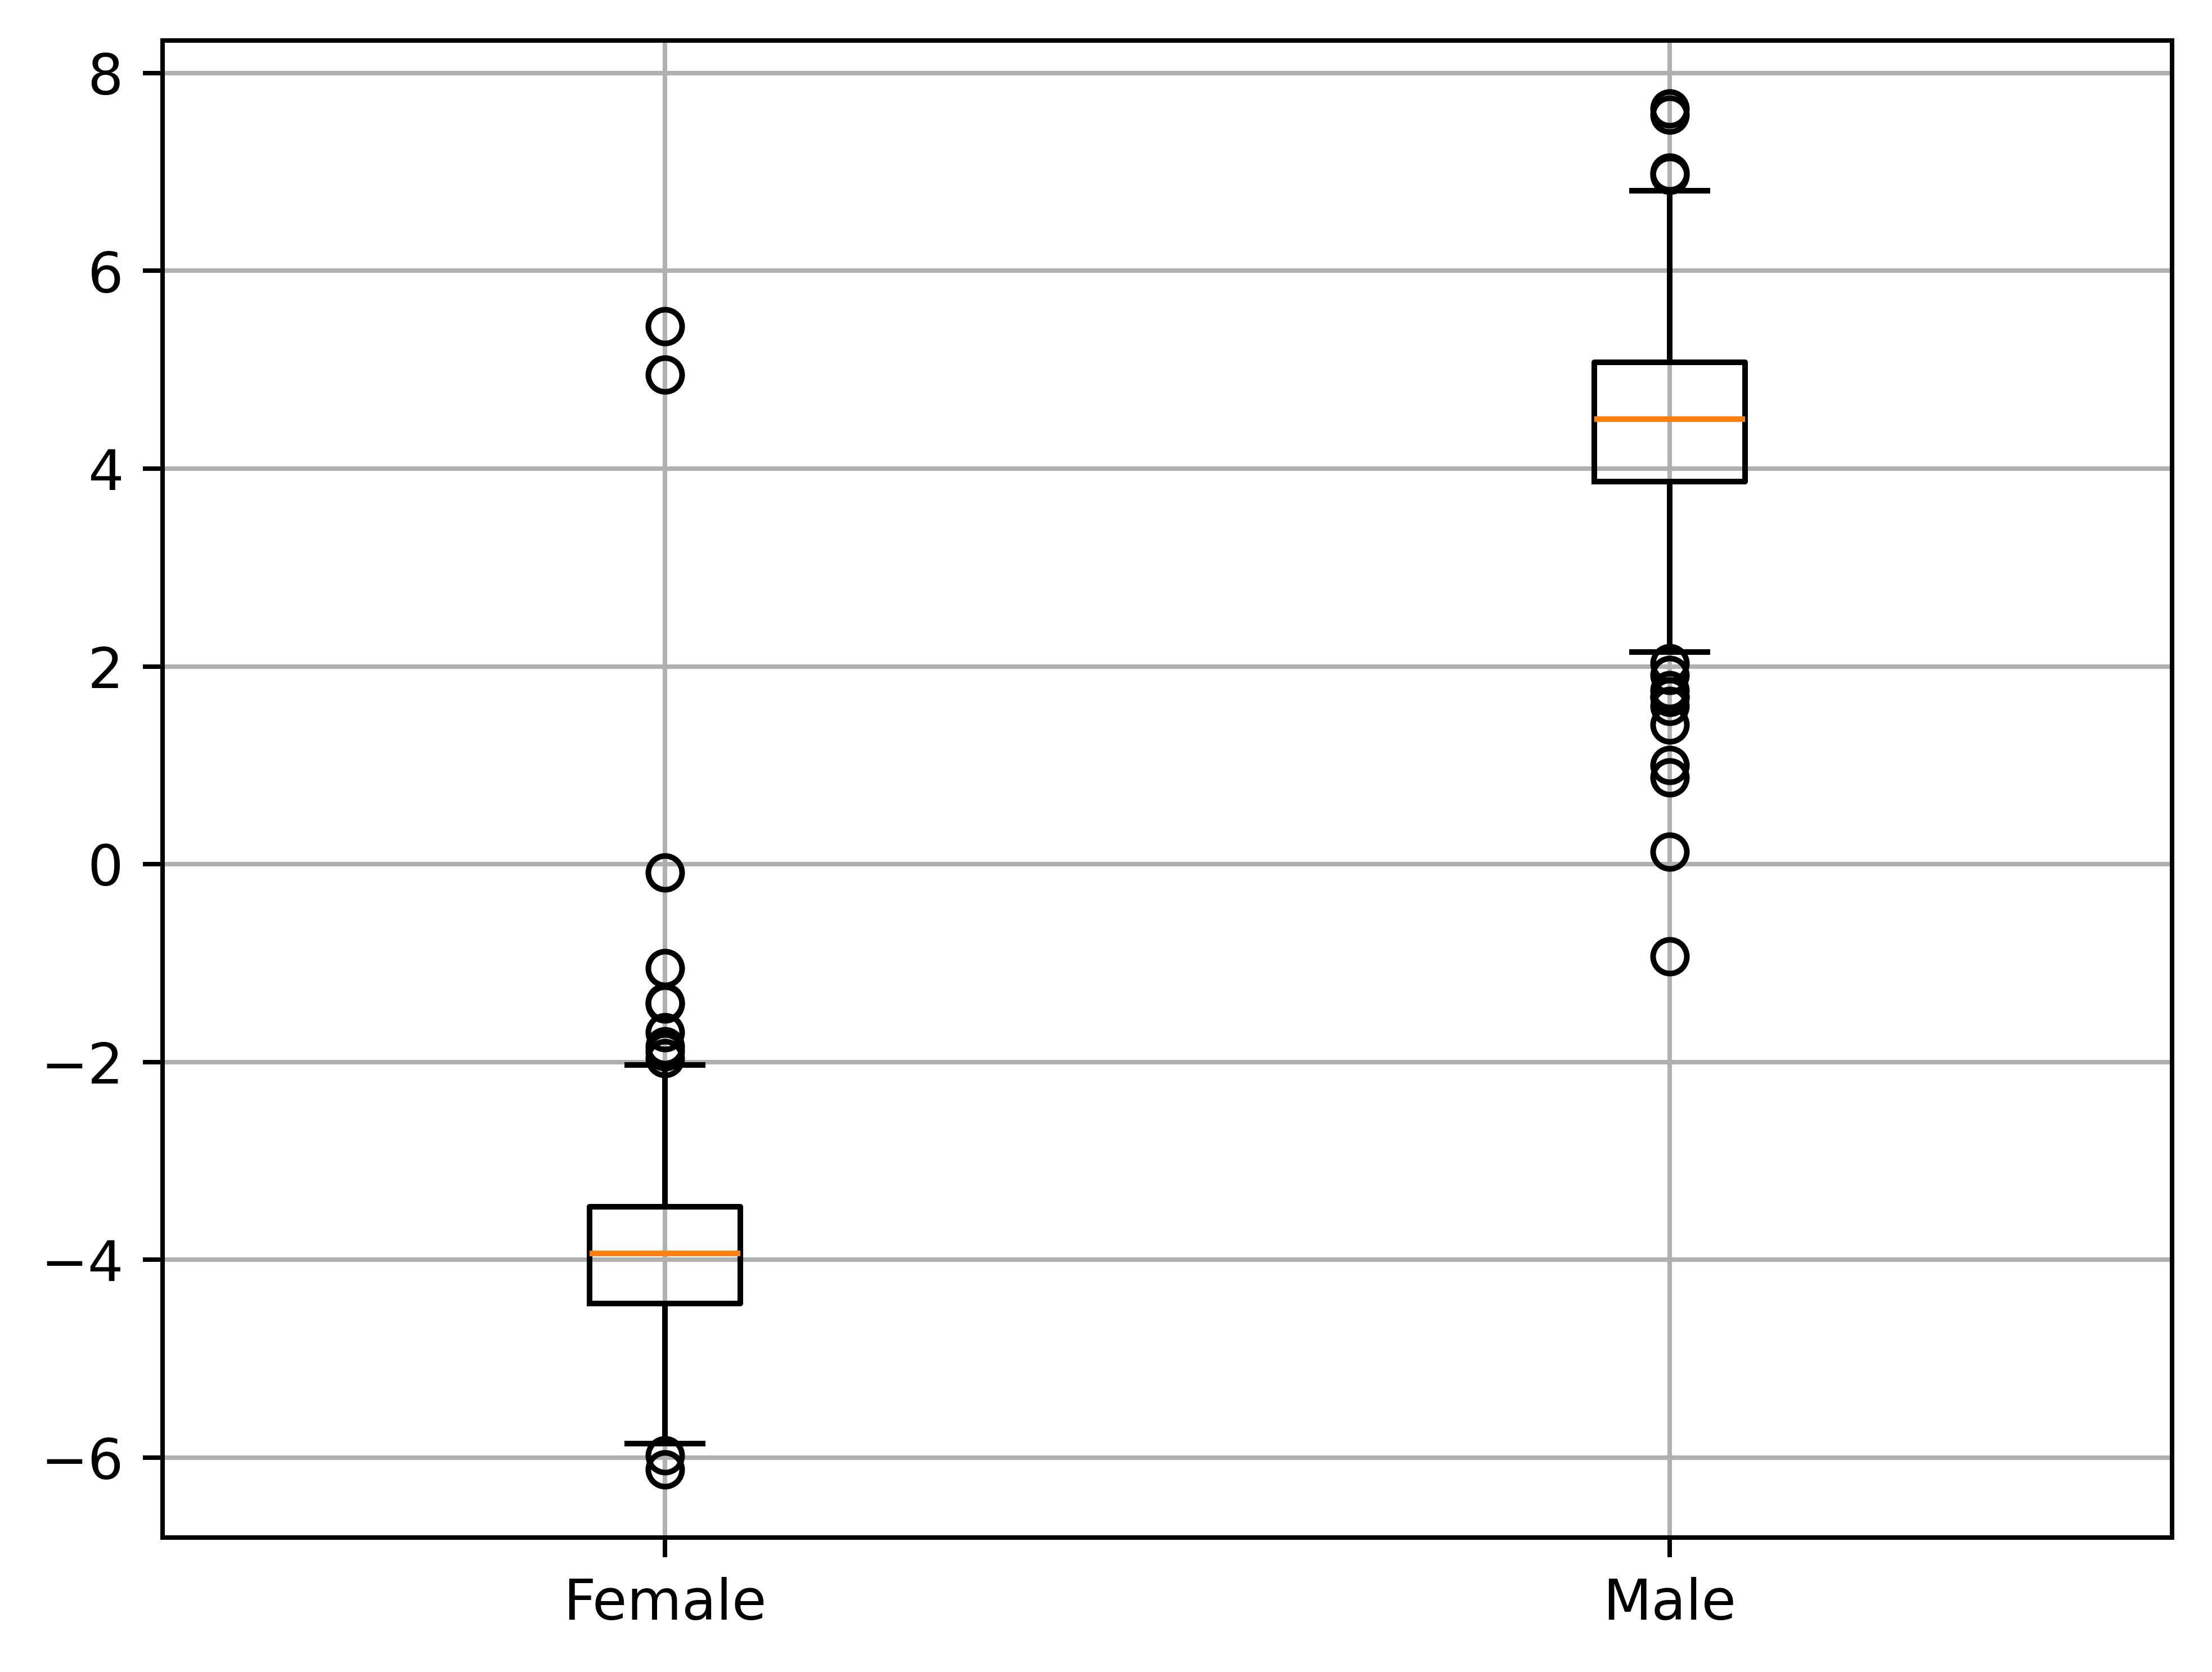
\includegraphics[width=0.4\textwidth]{../Analysis/LDA/node=50_size=480_step=180_rho=0.1/box_0.jpg}} \\
    \subfloat[]{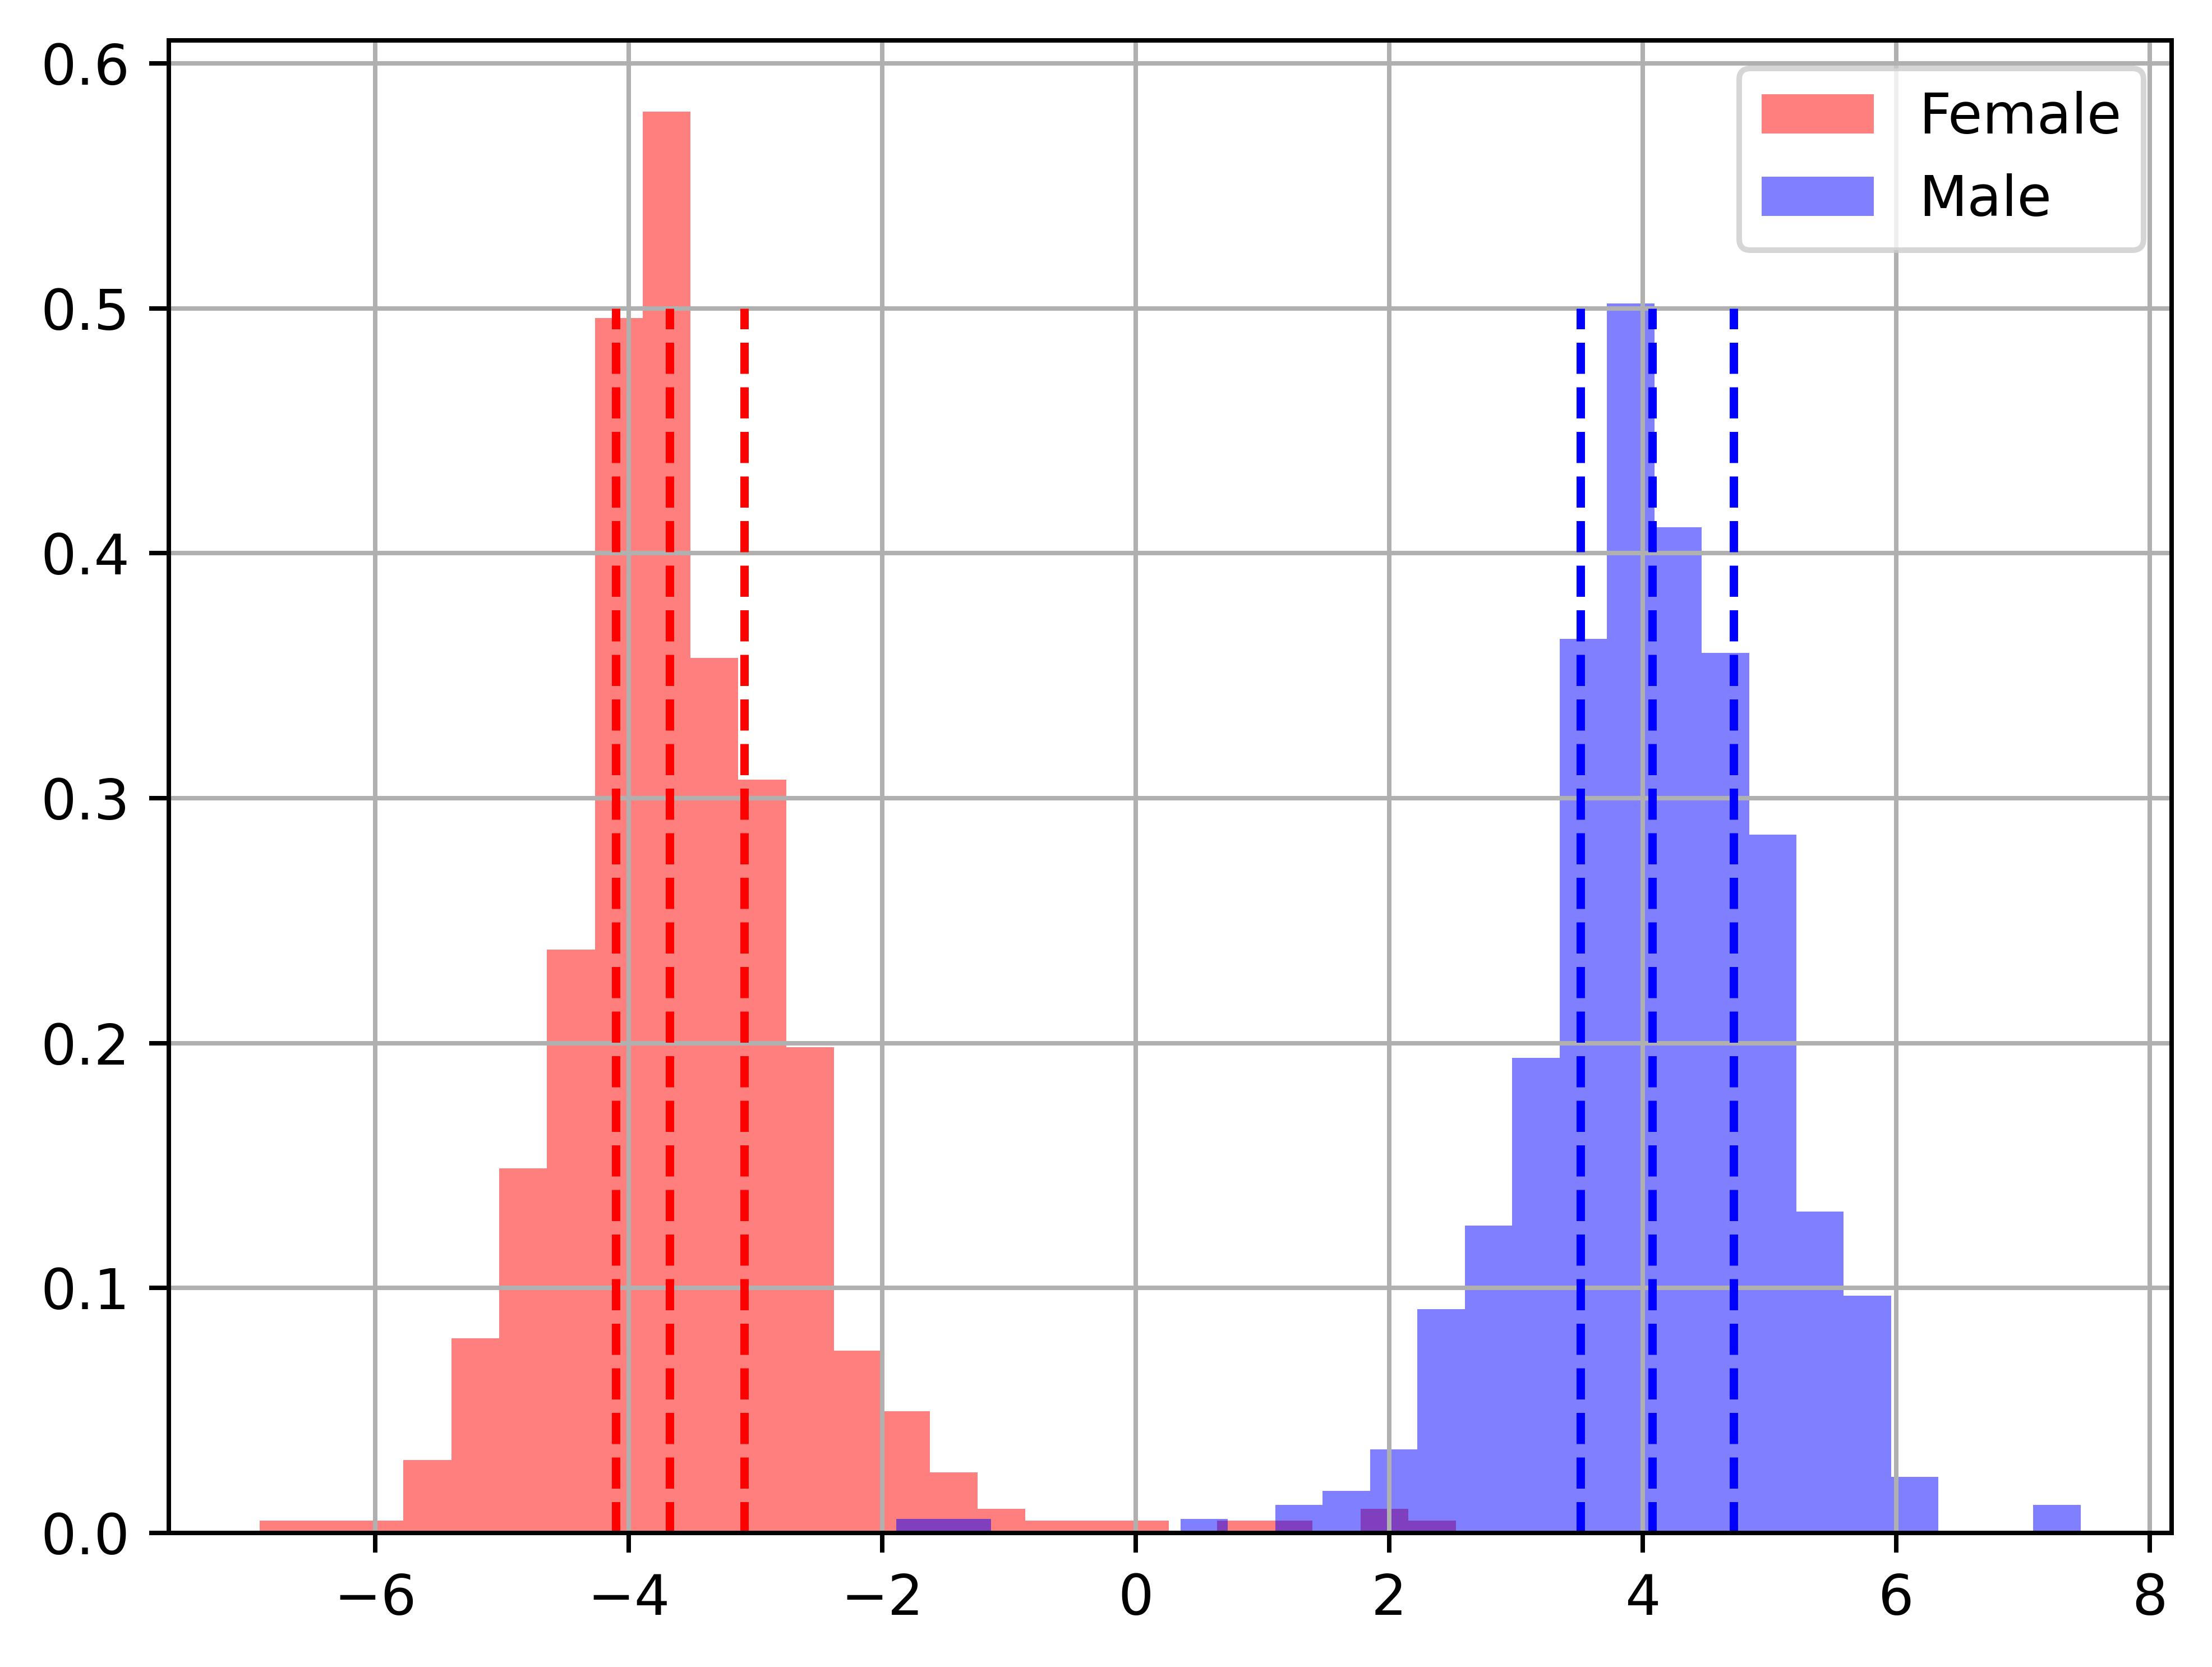
\includegraphics[width=0.4\textwidth]{../Analysis/LDA/node=50_size=480_step=180_rho=0.1/hist_1.jpg}}
    \subfloat[]{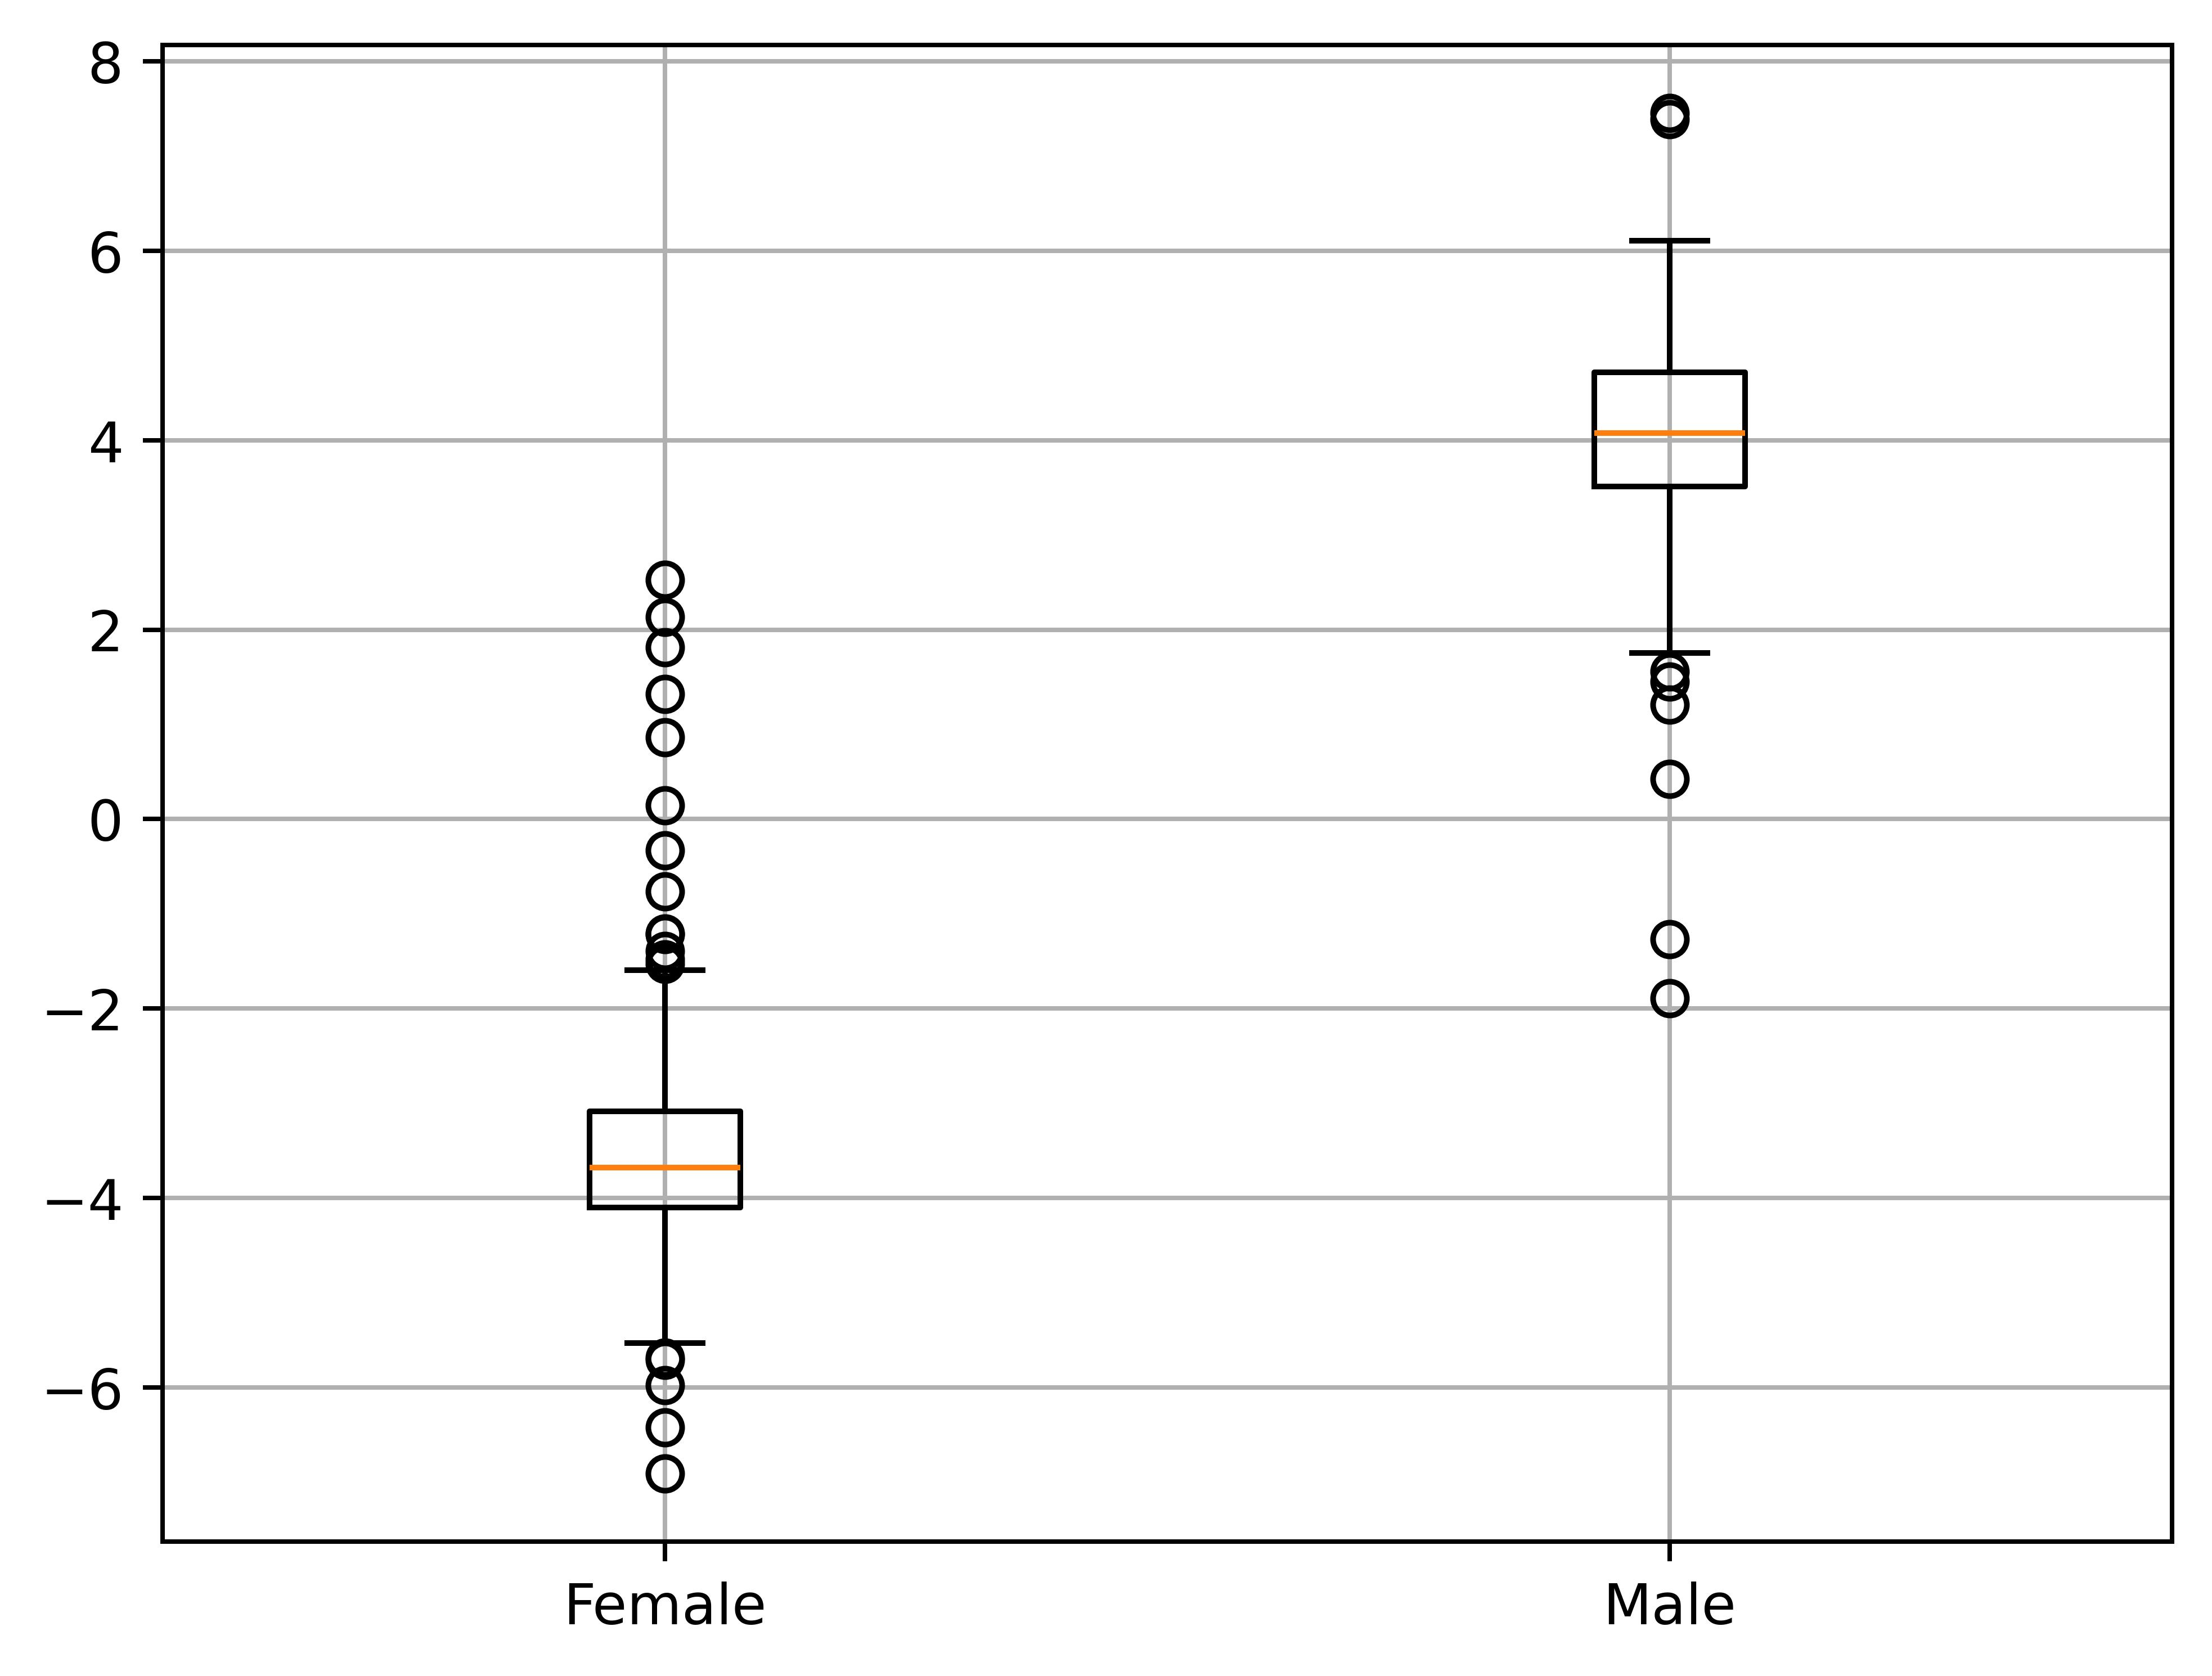
\includegraphics[width=0.4\textwidth]{../Analysis/LDA/node=50_size=480_step=180_rho=0.1/box_1.jpg}} \\
    \subfloat[]{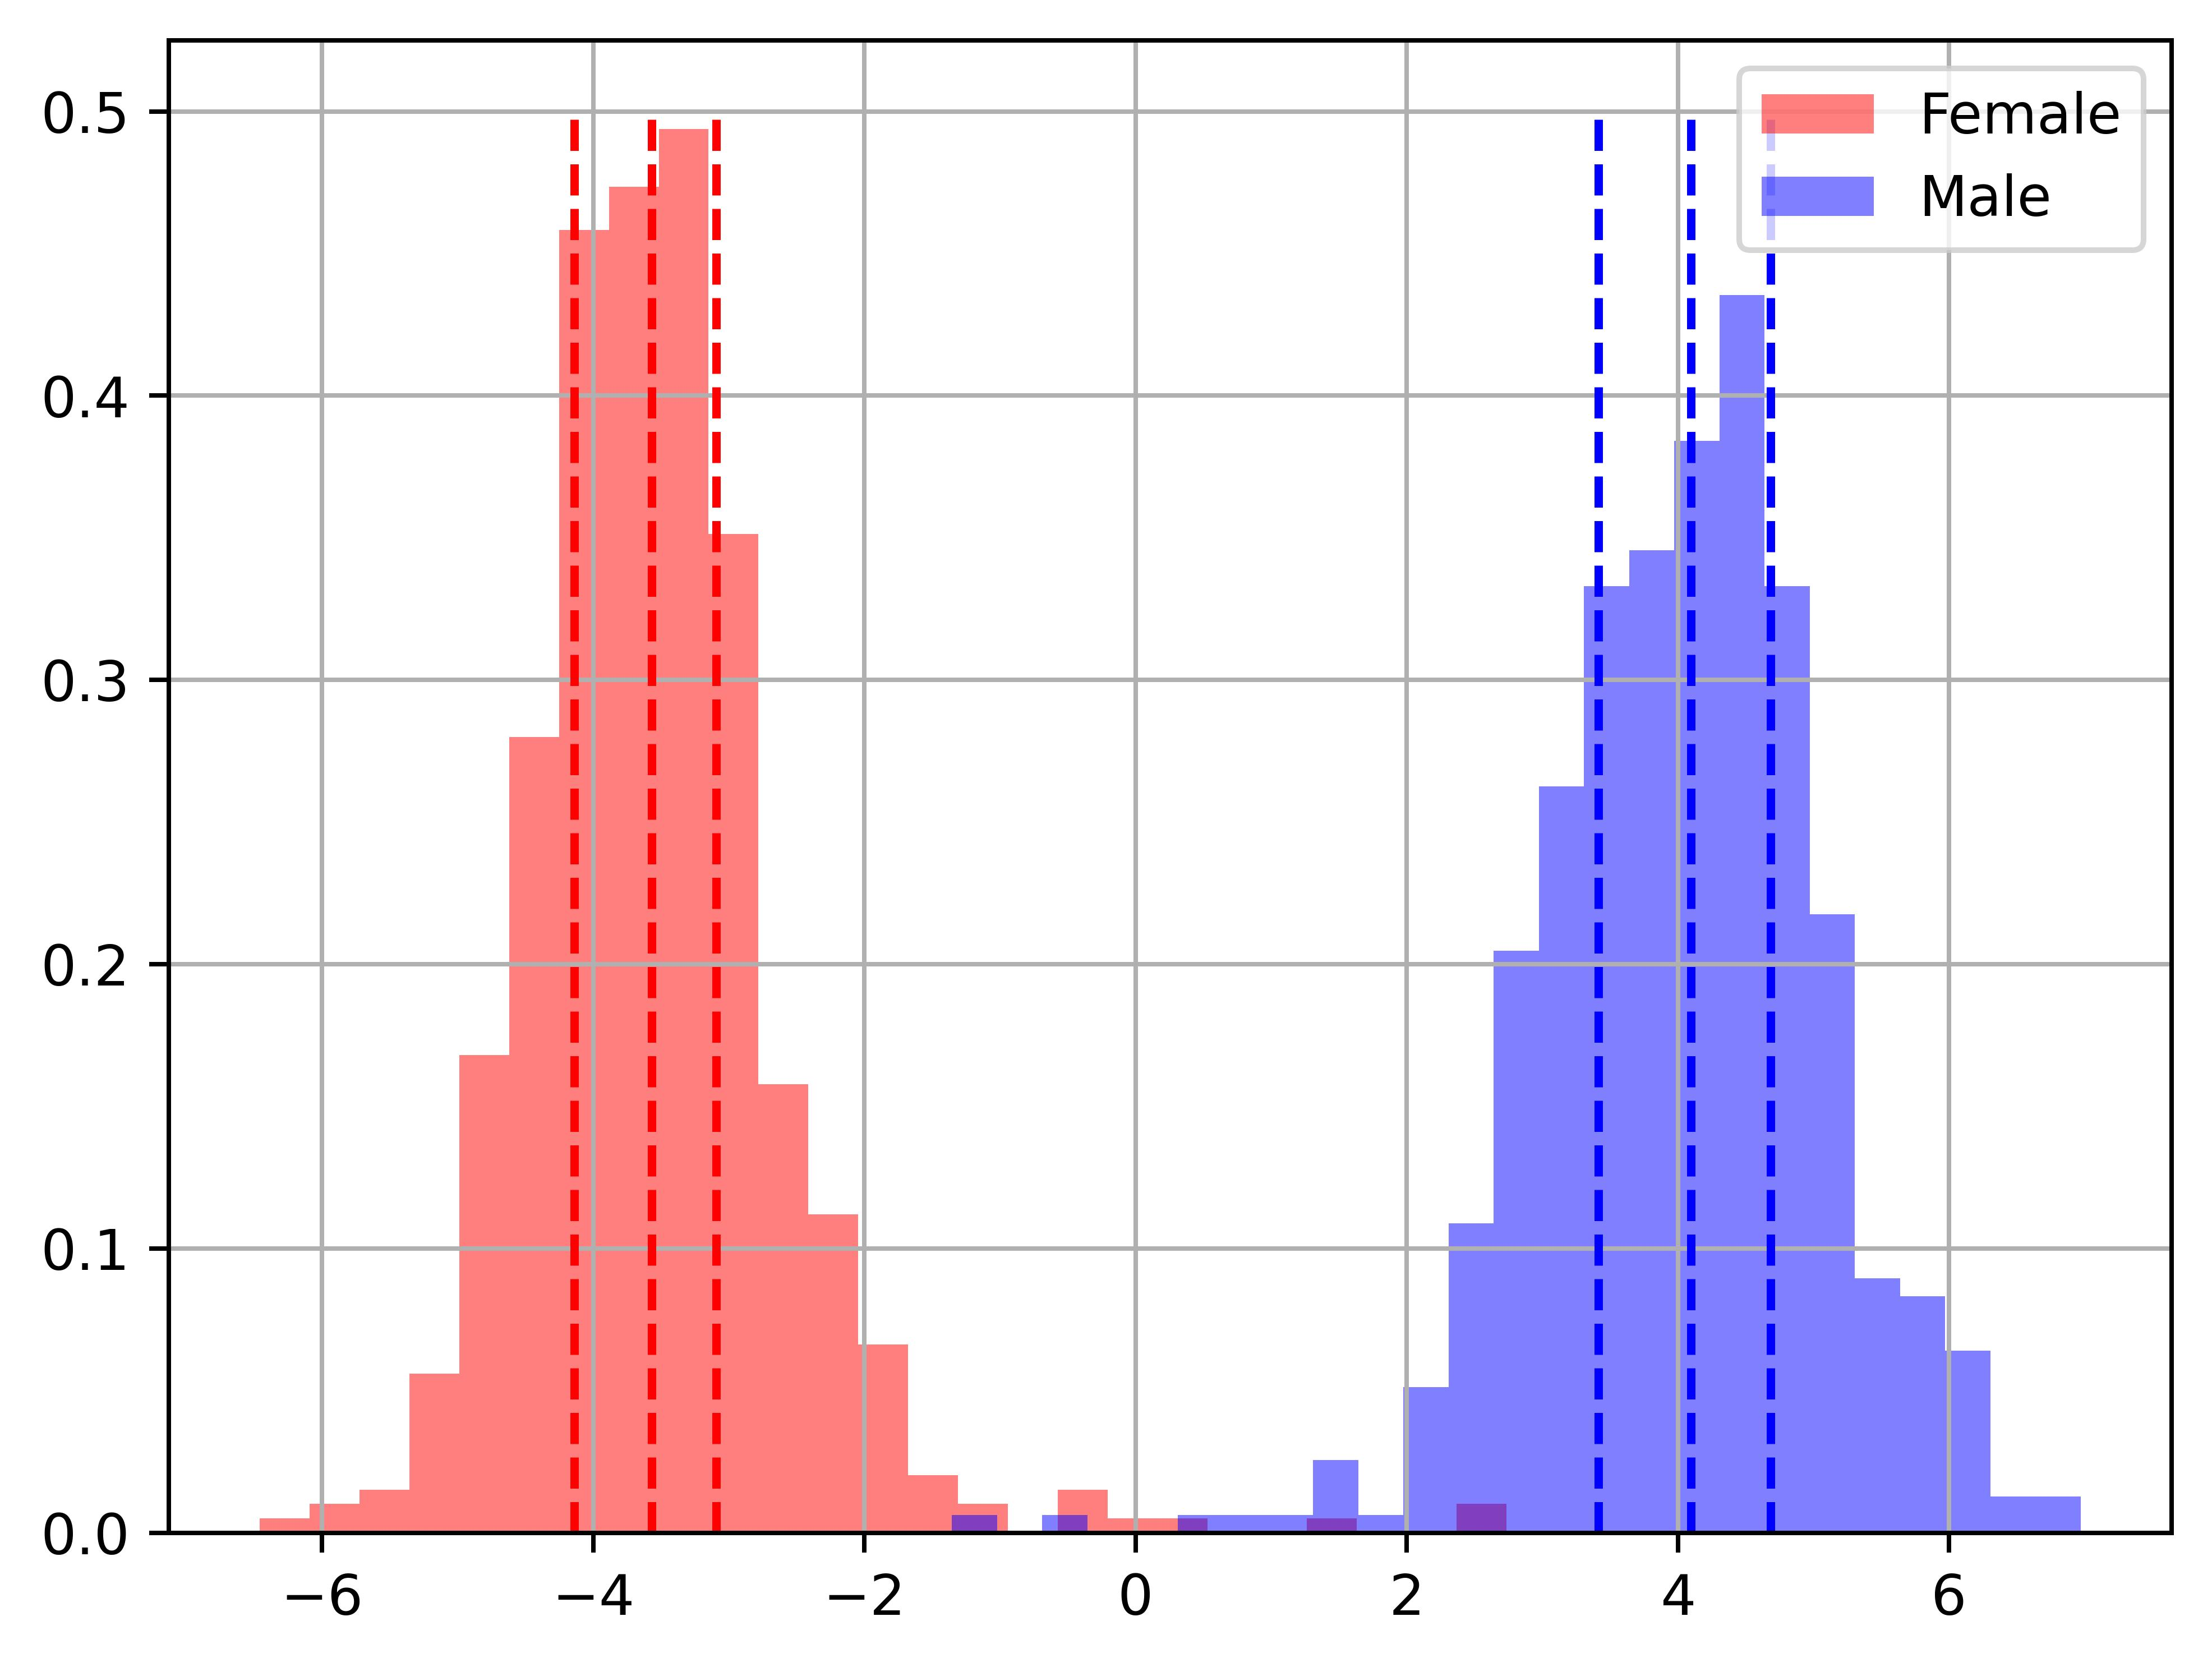
\includegraphics[width=0.4\textwidth]{../Analysis/LDA/node=50_size=480_step=180_rho=0.1/hist_2.jpg}}
    \subfloat[]{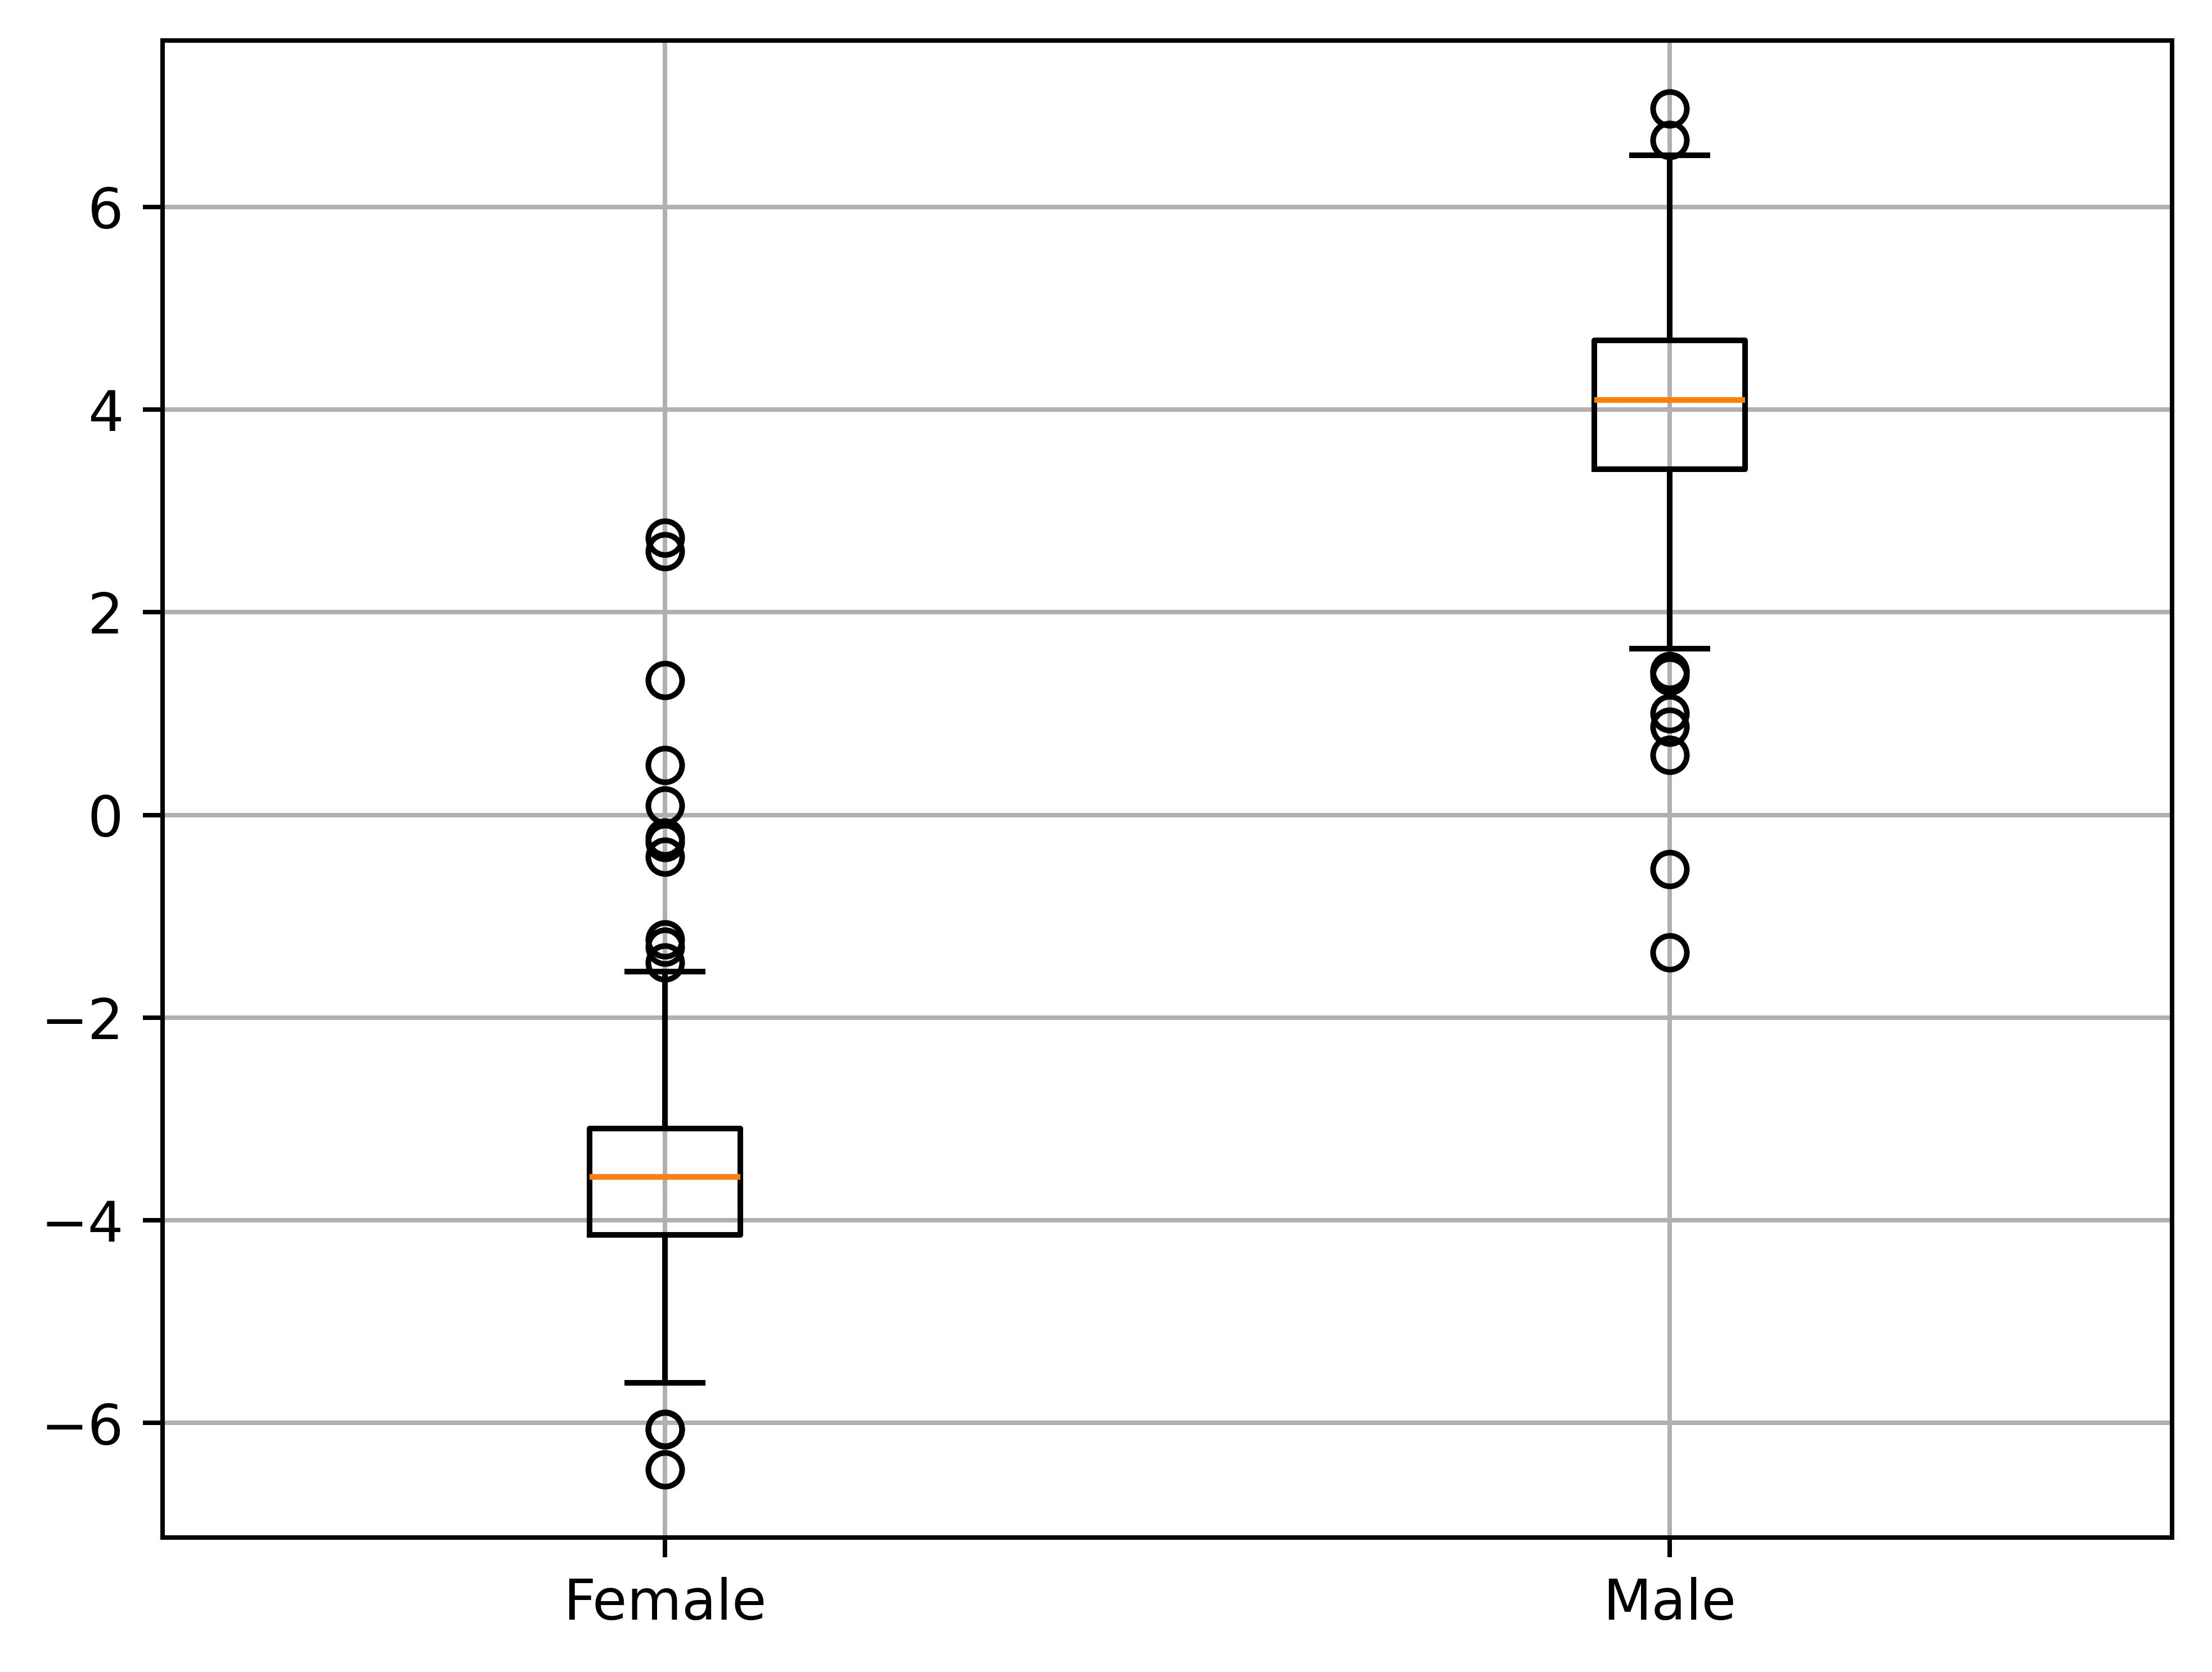
\includegraphics[width=0.4\textwidth]{../Analysis/LDA/node=50_size=480_step=180_rho=0.1/box_2.jpg}} \\
    \caption{LDA for Dynamic connectivity with $N_{node} = 50$.}
    \label{LDA-example-6}
\end{figure}

\subsection{SVM Model}

\begin{figure}[H]
    \centering
    \subfloat[]{\includegraphics[width=0.9\textwidth]{../SVM/bar.jpg}}
    \caption{Results of SVM model.}
    \label{SVM-results-1}
\end{figure}

\subsection{CNN Model}

\begin{figure}[H]
    \centering
    \subfloat[dropout = 0.0]{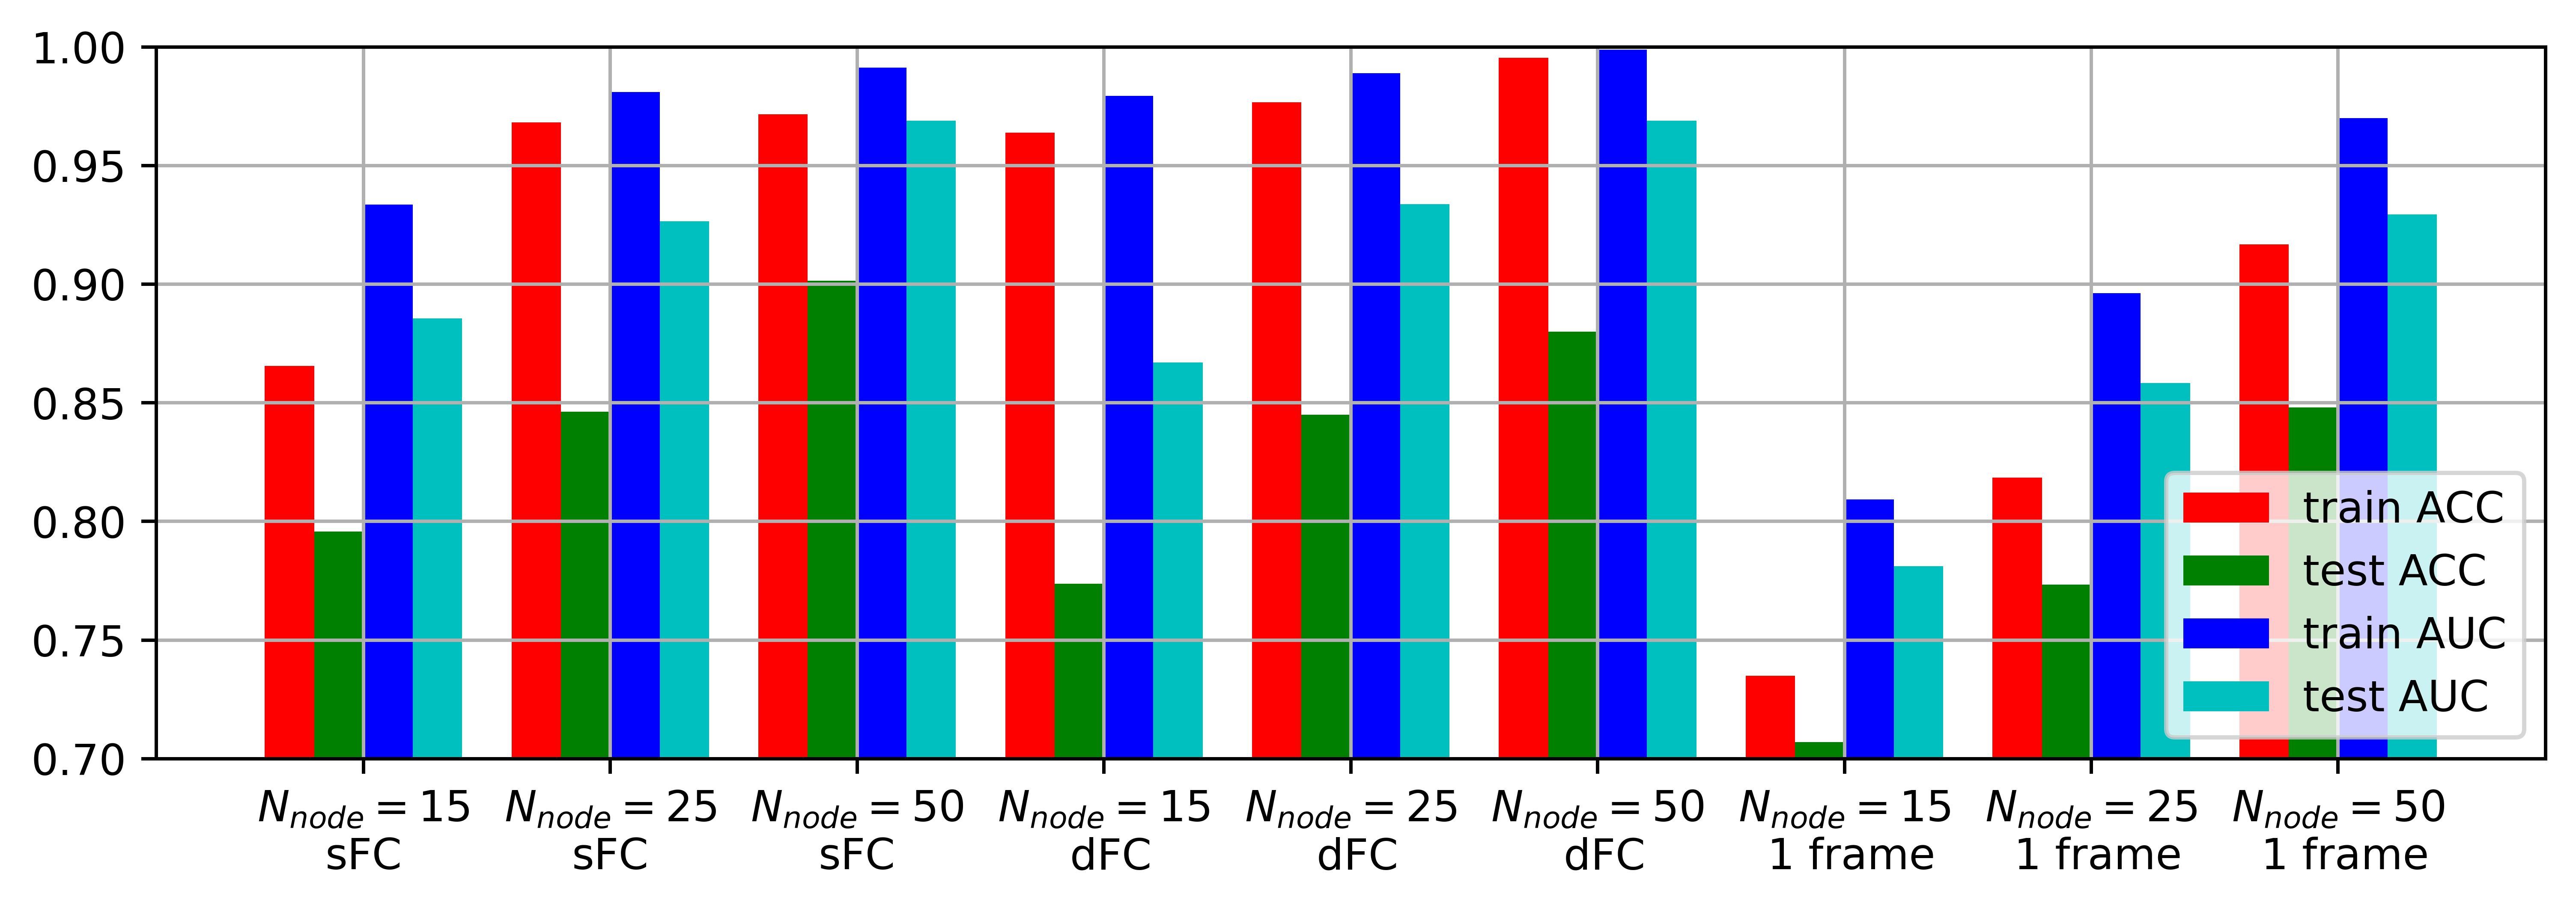
\includegraphics[width=0.9\textwidth]{../output/bar_channel=1_dropout=0.0.jpg}} \\
    \subfloat[dropout = 0.1]{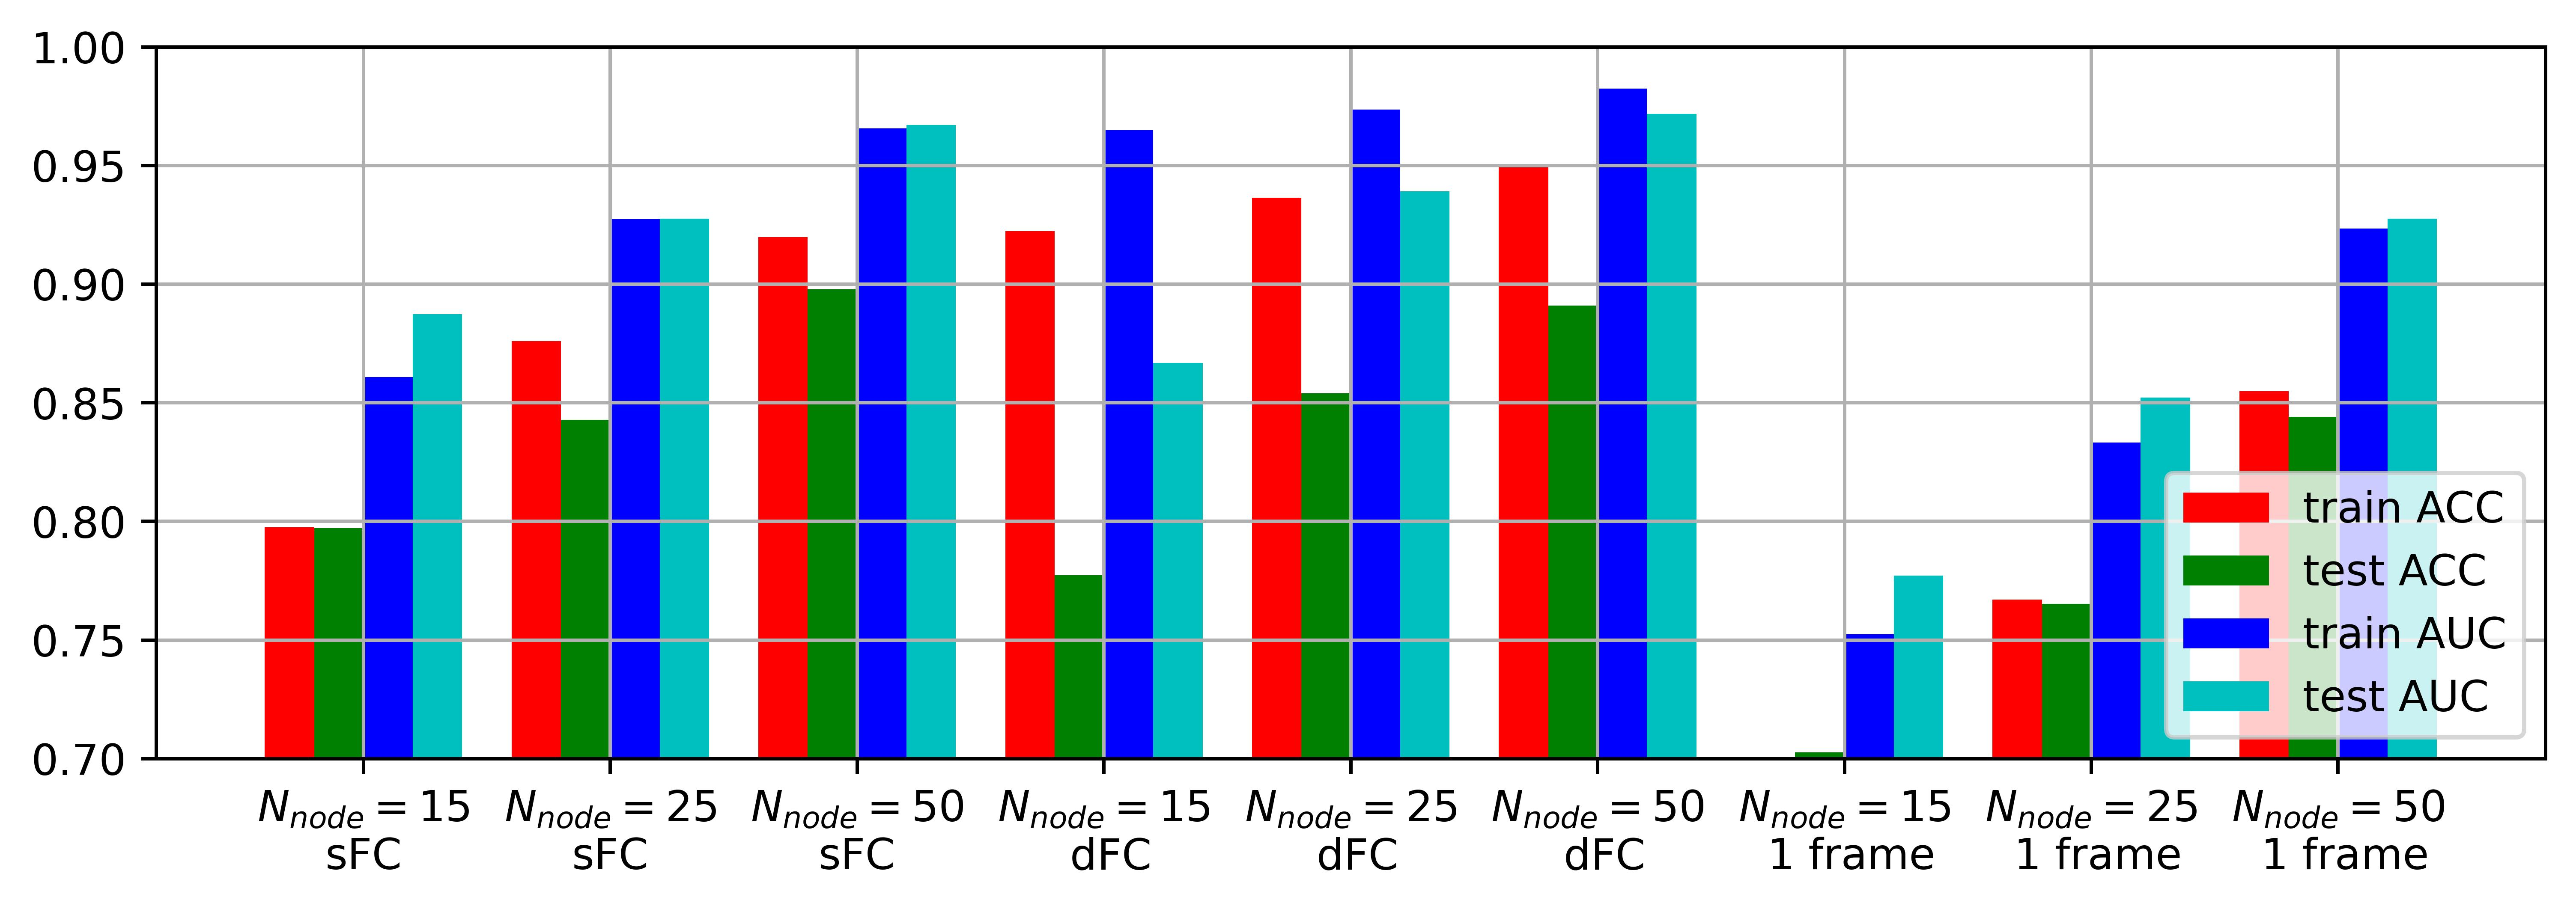
\includegraphics[width=0.9\textwidth]{../output/bar_channel=1_dropout=0.1.jpg}} \\
    \caption{Results of CNN model with channel = 1.}
    \label{CNN-results-1}
\end{figure}

\begin{figure}[H]
    \centering
    \subfloat[dropout = 0.0]{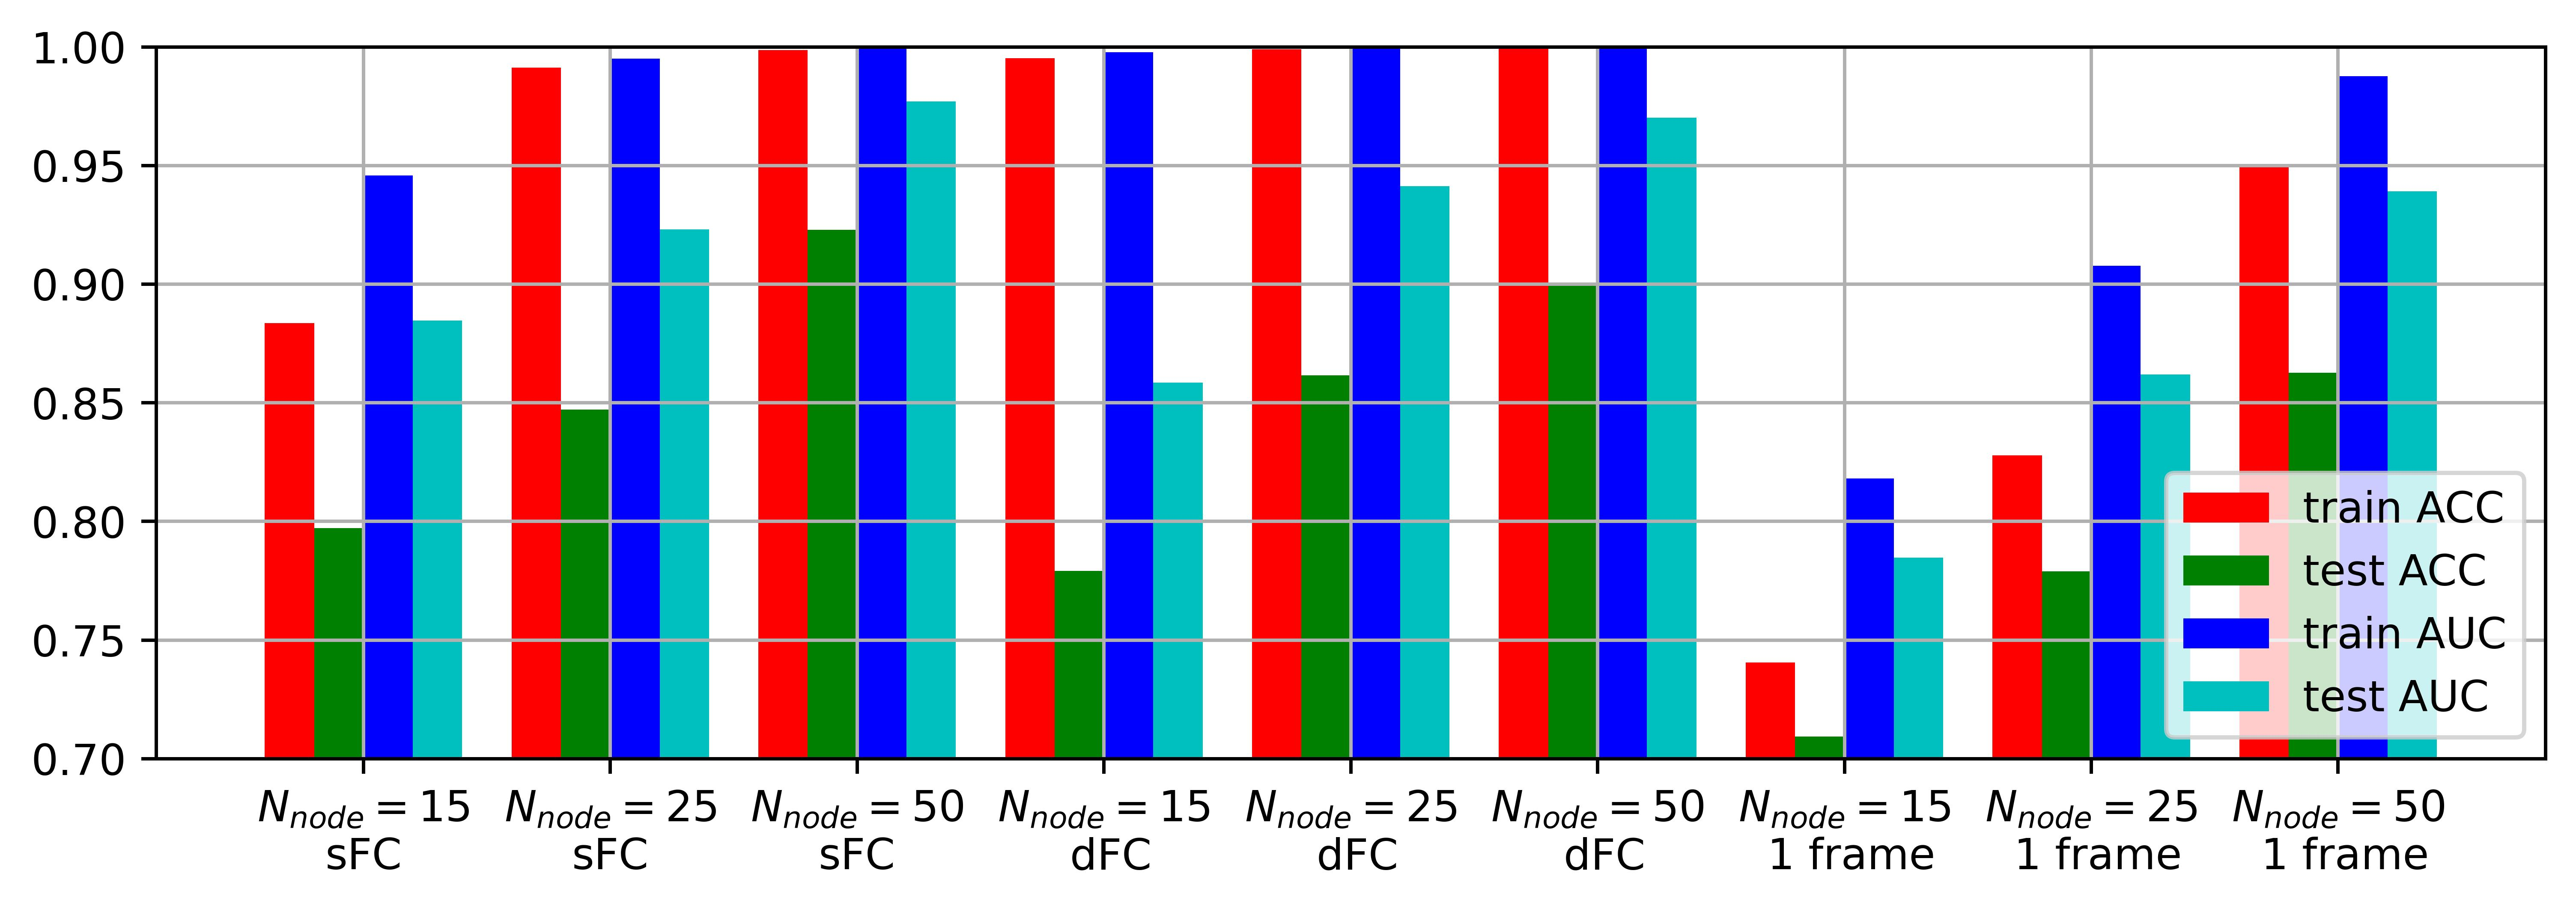
\includegraphics[width=0.9\textwidth]{../output/bar_channel=2_dropout=0.0.jpg}} \\
    \subfloat[dropout = 0.1]{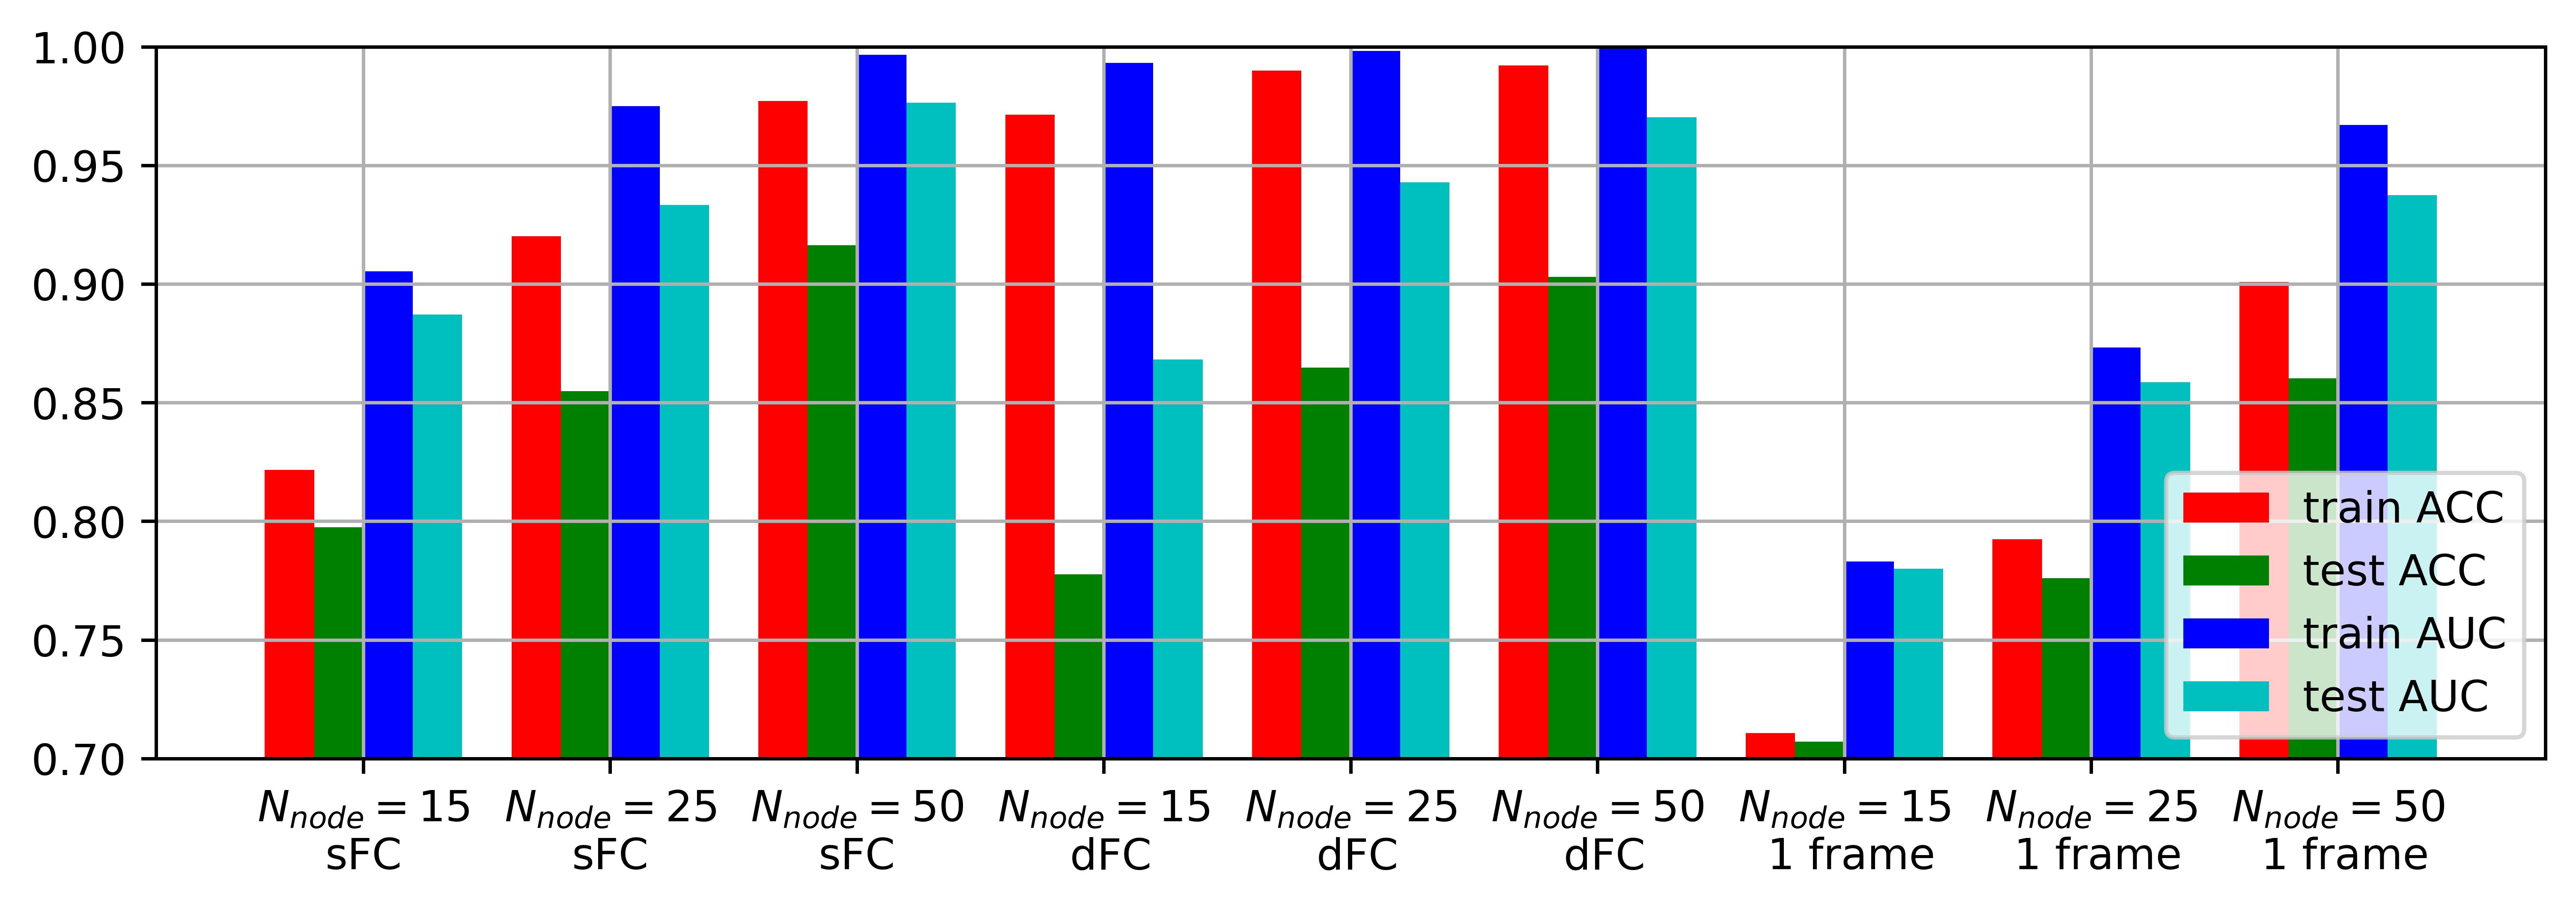
\includegraphics[width=0.9\textwidth]{../output/bar_channel=2_dropout=0.1.jpg}} \\
    \caption{Results of CNN model with channel = 2.}
    \label{CNN-results-2}
\end{figure}

\begin{figure}[H]
    \centering
    \subfloat[dropout = 0.0]{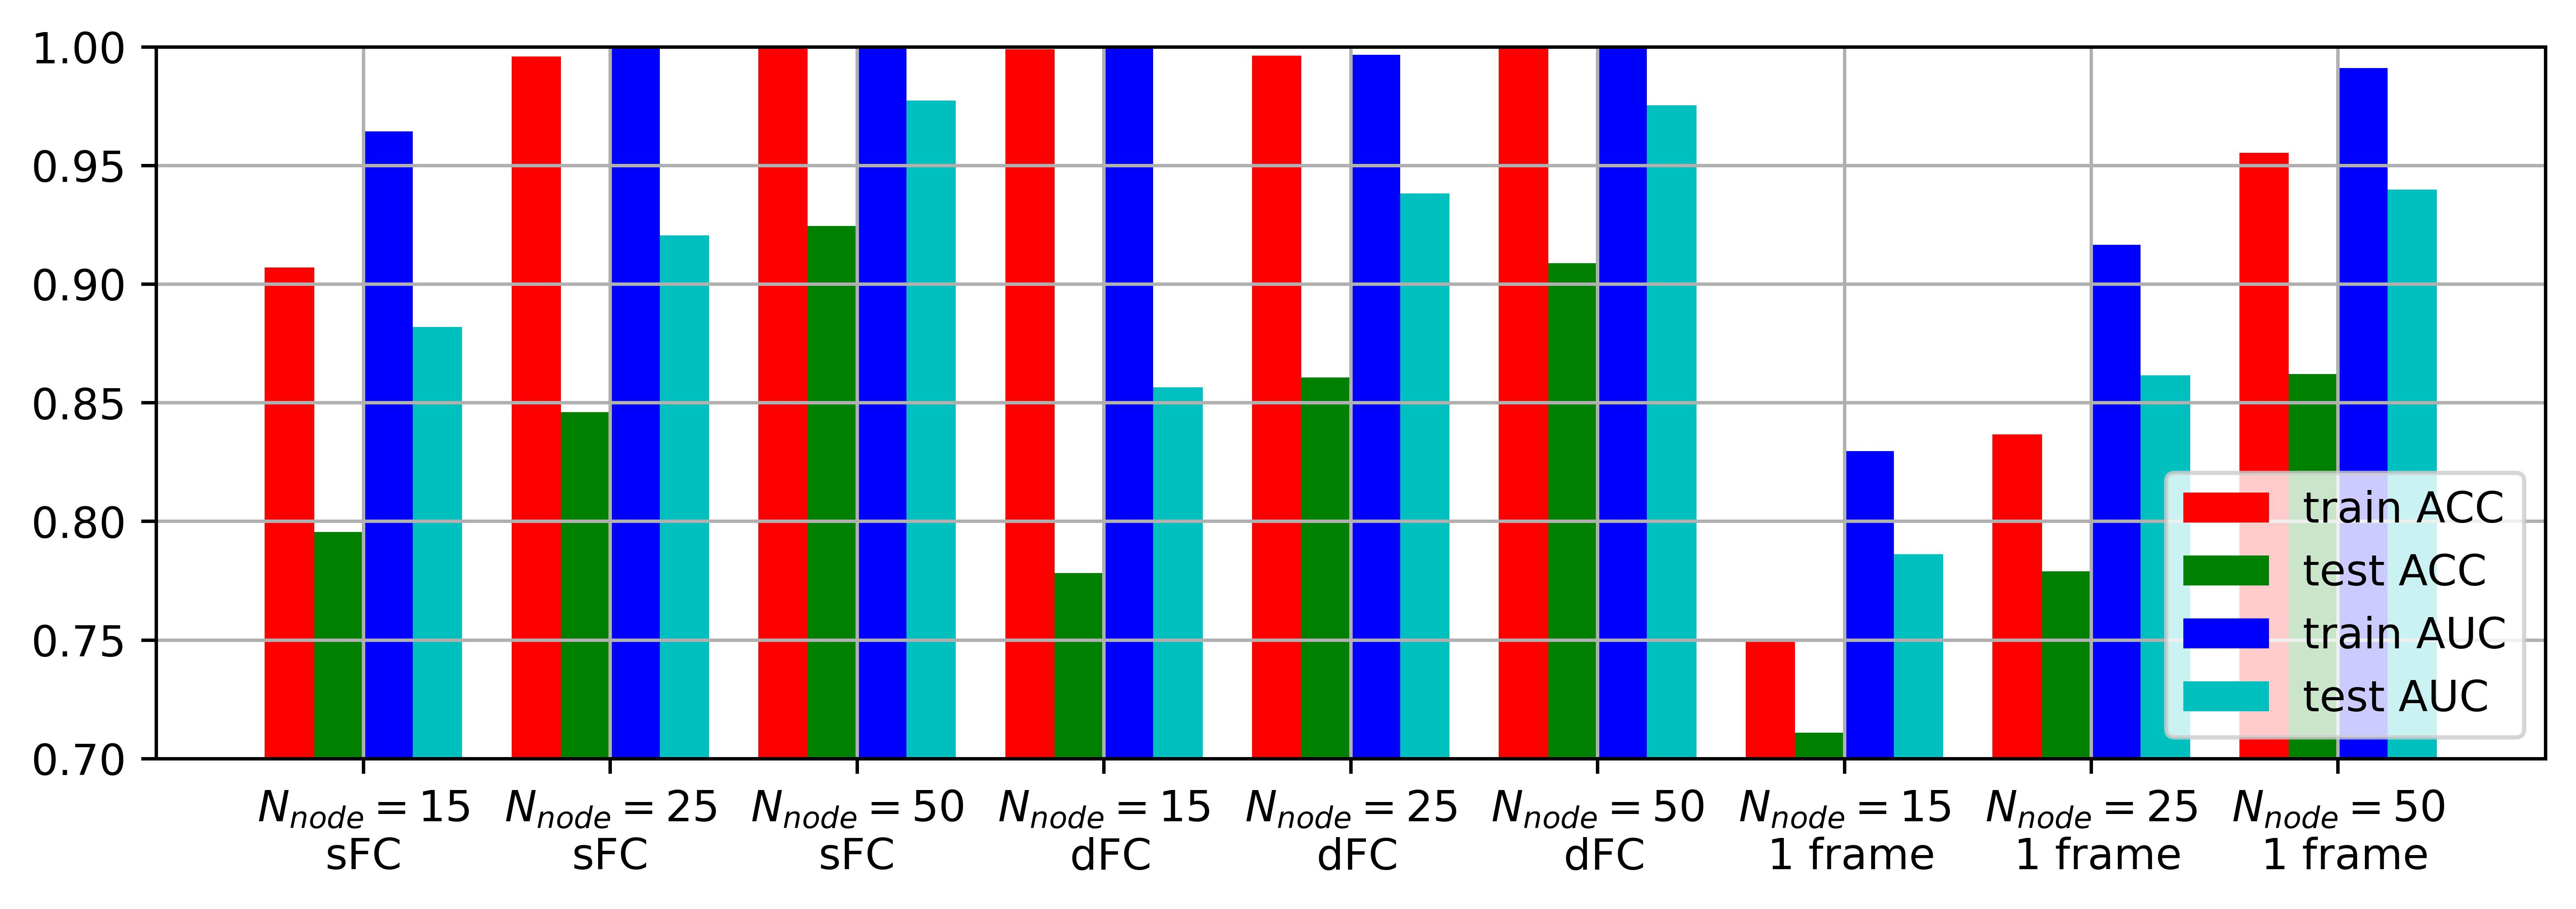
\includegraphics[width=0.9\textwidth]{../output/bar_channel=4_dropout=0.0.jpg}} \\
    \subfloat[dropout = 0.1]{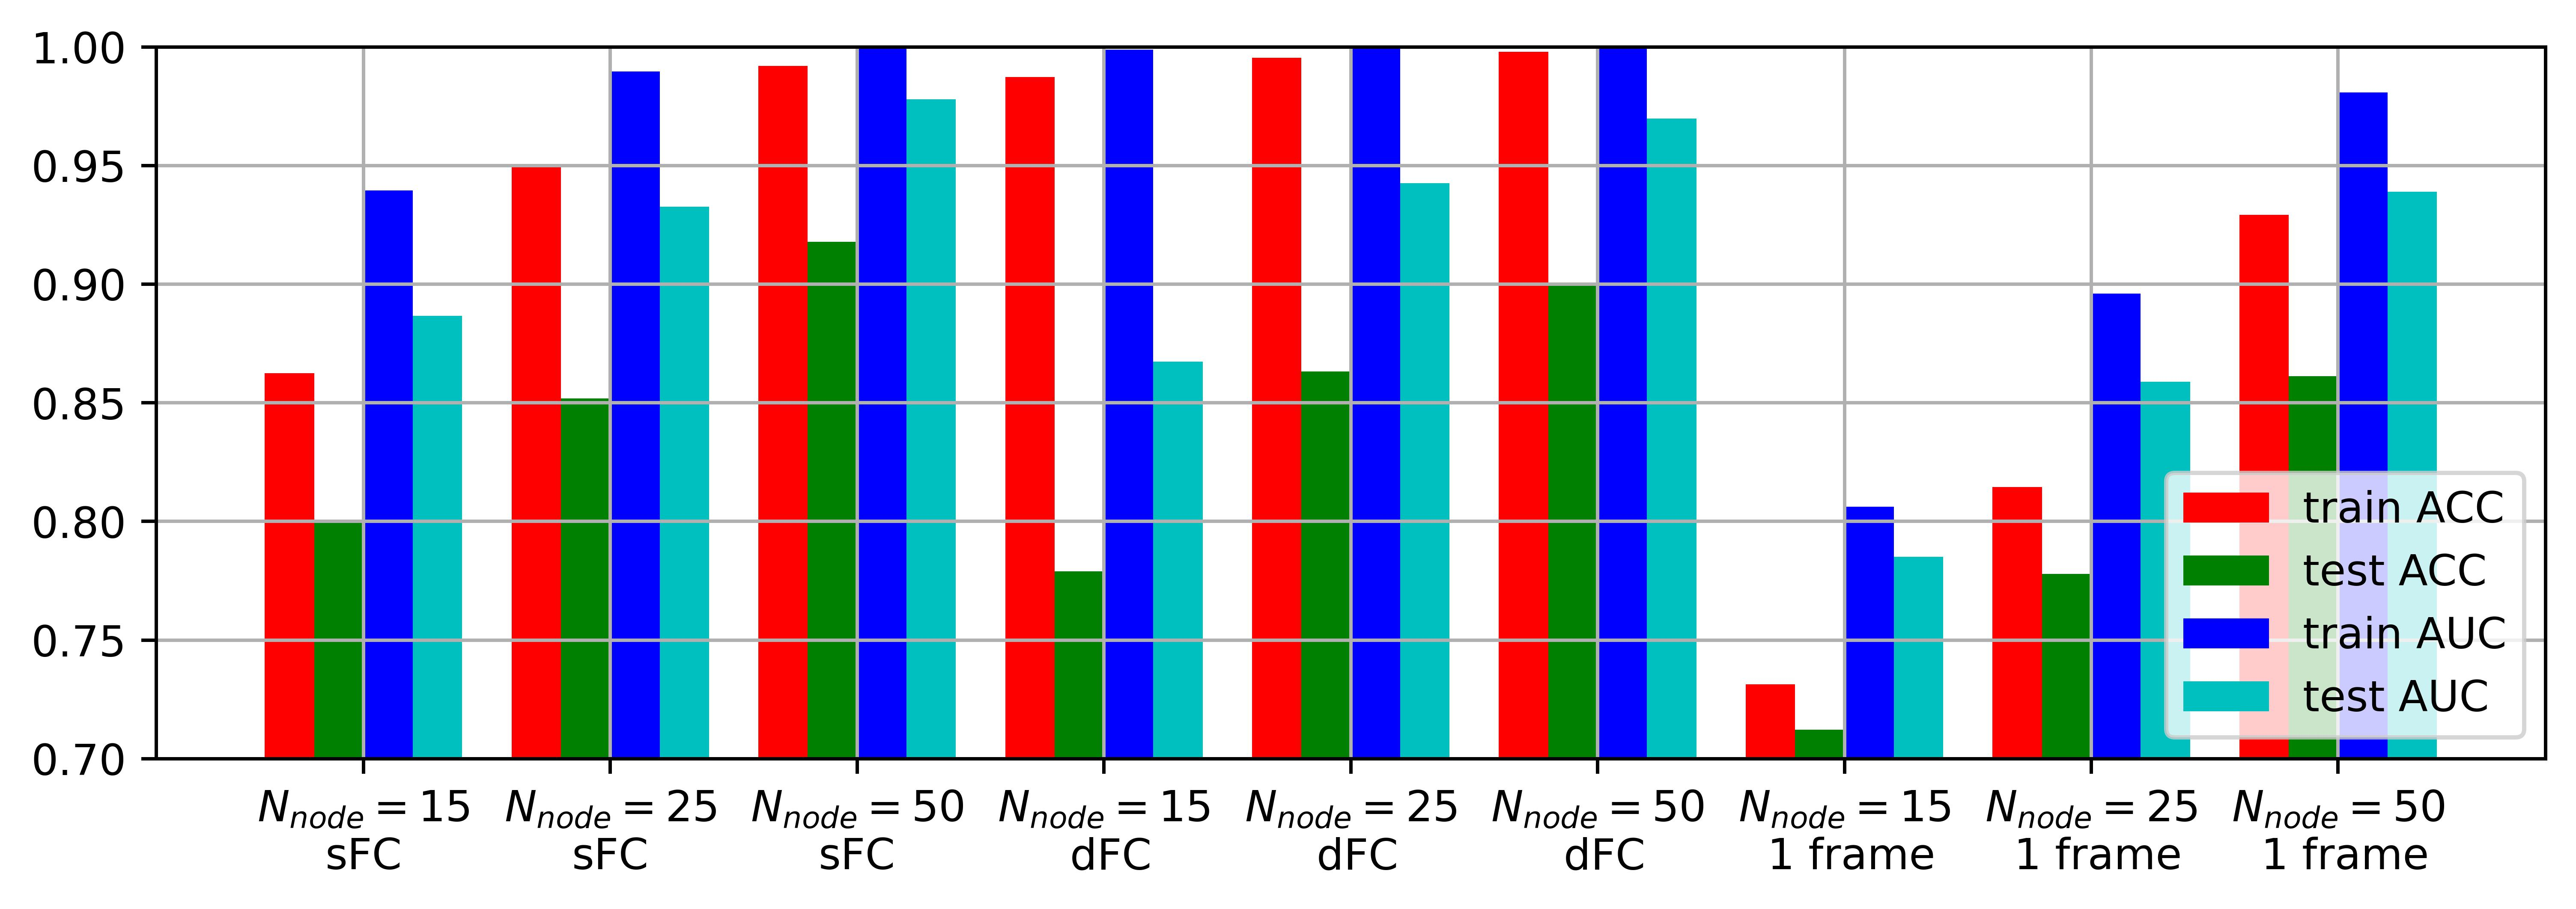
\includegraphics[width=0.9\textwidth]{../output/bar_channel=4_dropout=0.1.jpg}} \\
    \caption{Results of CNN model with channel = 4.}
    \label{CNN-results-3}
\end{figure}

\section{Results}

\section{Discussion}

% \newpage

% \begin{thebibliography}{99}
% \addcontentsline{toc}{section}{参考文献}

% \end{thebibliography}

% \newpage

% \appendix
% \renewcommand\thesection{\Alph{section}}

\end{document}